\documentclass[compress]{beamer}

\usetheme{Luebeck}
\usepackage[utf8]{inputenc}
\usepackage{subfig}
\usepackage{utopia} %font utopia imported
\usepackage{arabtex}
\usepackage{utf8}
\setcode{utf8}
\usepackage{amsmath}
\usepackage{amssymb}
\usepackage{amsthm}
\usepackage{textcomp}
\usefonttheme{professionalfonts} % using non standard fonts for beamer
\definecolor{foo}{RGB}{106,141,143}
\usecolortheme[named=foo]{structure}
\setbeamercolor{subsection in head/foot}{bg=foo!80!black}
% This block of code defines the information to appear in the
% title page

\title[ASIC Physical Design] %optional
{Routing}

\subtitle{How to Route your own chip}

\author[Ahmed Abdelazeem] % (optional)
{Ahmed Abdelazeem}
%{A.~B.~Arthur\inst{1} \and J.~Doe\inst{2}}

\institute[ZU] % (optional)
{
	Faculty of Engineering\\
	Zagazig University
}
%{
	%	\inst{1}%
	%	Faculty of Engineering\\
	%	Zagazig University
	%	\and
	%	\inst{2}%
	%	Faculty of Chemistry\\
	%	Very Famous University
	%}

\date[ZU 2023] % (optional)
{RTL2GDSII Flow, March 2022}

%\logo{
\includegraphics[height=1.5cm]{lion-logo.png}}

%End of title page configuration block
%------------------------------------------------------------

%------------------------------------------------------------
%The next block of commands puts the table of contents at the
%beginning of each section and highlights the current section:
\setcounter{tocdepth}{1} %%%
\AtBeginSection[]
{
	\begin{frame}
		\frametitle{Table of Contents}
		\tableofcontents[currentsection]
	\end{frame}
}
%------------------------------------------------------------


\begin{document}
	
	%The next statement creates the title page.
	\frame{\titlepage}
	
	
	%---------------------------------------------------------
	%This block of code is for the table of contents after
	%the title page
	\begin{frame}
		\frametitle{Table of Contents}
		\tableofcontents
	\end{frame}
	%---------------------------------------------------------
	%--------------------------------------------------
	\section[Intro]{Introduction}
	\subsection[Routing]{Routing}
	\begin{frame}
		\frametitle{Design Status, Start of Routing Phase}
		\begin{itemize}
			\item \textbf{Placement - completed}
			\item \textbf{CTS – completed}
			\item \textbf{Power and ground nets – prerouted}
			\item \textbf{Estimated congestion - acceptable}
			\item \textbf{Estimated timing - acceptable (~0ns slack)}
			\item \textbf{Estimated max cap/transition – no violations}
		\end{itemize}
	
	\end{frame}	
	\subsection[Route]{Routing Problem}
	\begin{frame}
		\frametitle{Routing Fundamentals: Goal}
		\begin{center}
			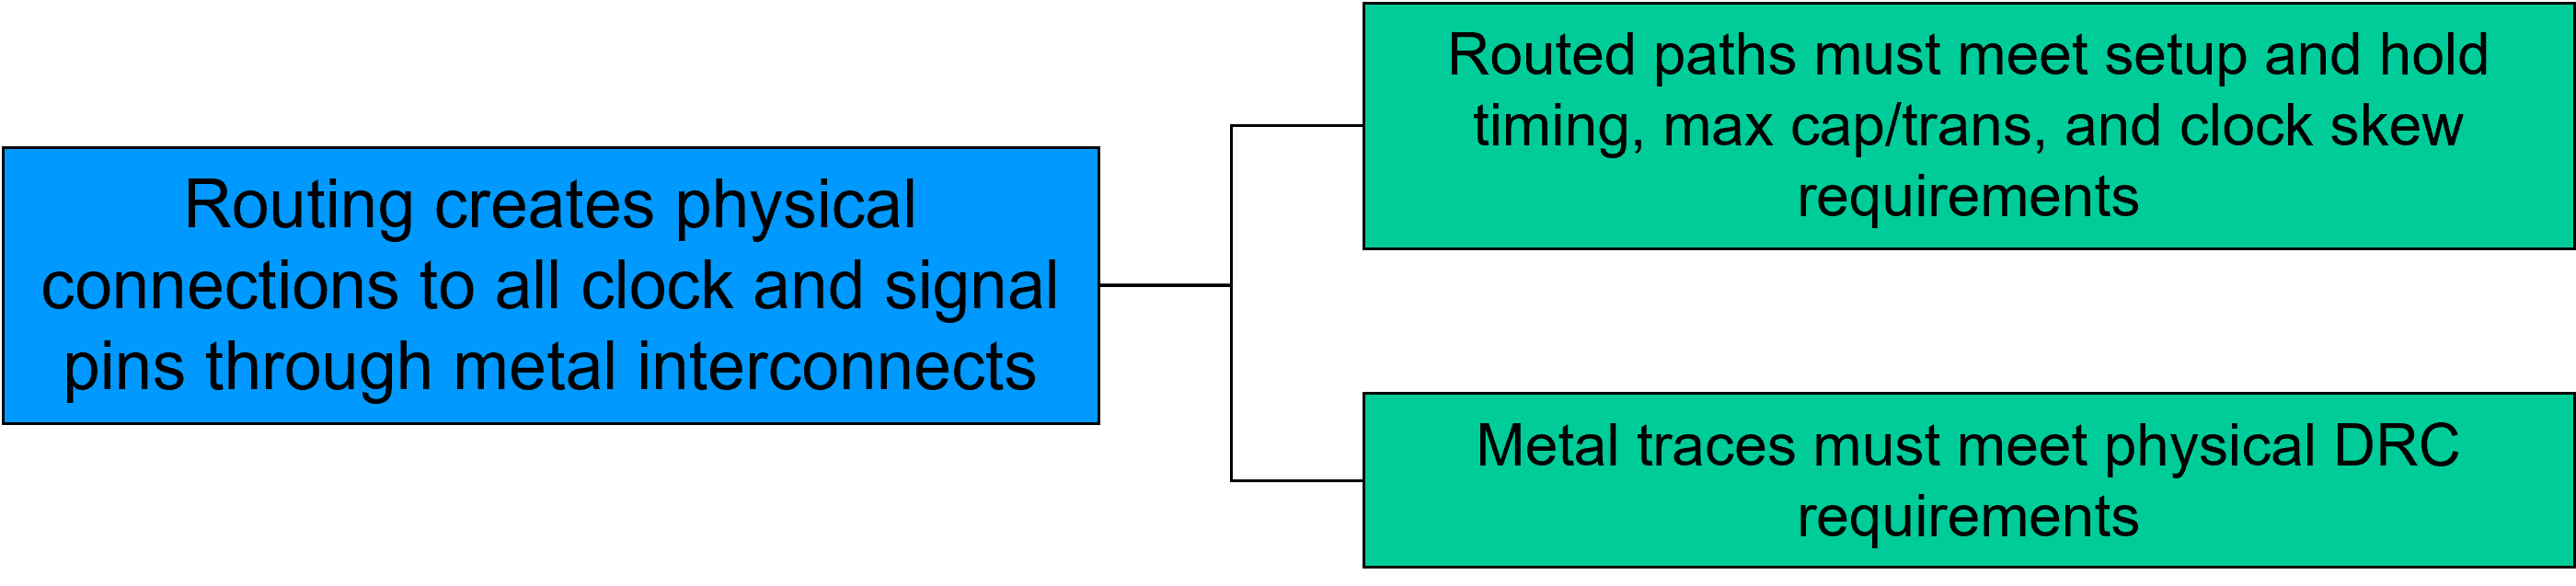
\includegraphics[width=0.8\textwidth]{Route}
		\end{center}
	\textbf{Routing creates physical connections to all clock and signal pins through metal interconnects}
		\begin{itemize}
			\item \textcolor{red}{Routed paths must meet setup and hold timing, max
				cap/trans, and clock skew requirements}
			\item \textcolor{red}{Metal traces must meet physical DRC requirements}

		\end{itemize}
			
	\end{frame}
	
	\begin{frame}
		\frametitle{Grid-Based Routing System}
		\begin{columns}	
			\column{0.6\textwidth}
		\begin{itemize}
			\item \textbf{Metal traces (routes) are built along and centered upon routing tracks based on a grid.}
			\item \textbf{Each metal layer has its own grid and preferred routing direction:}
			\begin{itemize}
				\item M1: Horizontal
				\item M2: Vertical, etc…
			\end{itemize}
			\item \textbf{The tracks and preferred routing directions are defined in a "unitTile" cell in the standard cell library}		
		\end{itemize}
	\column{0.6\textwidth}
		\begin{center}
			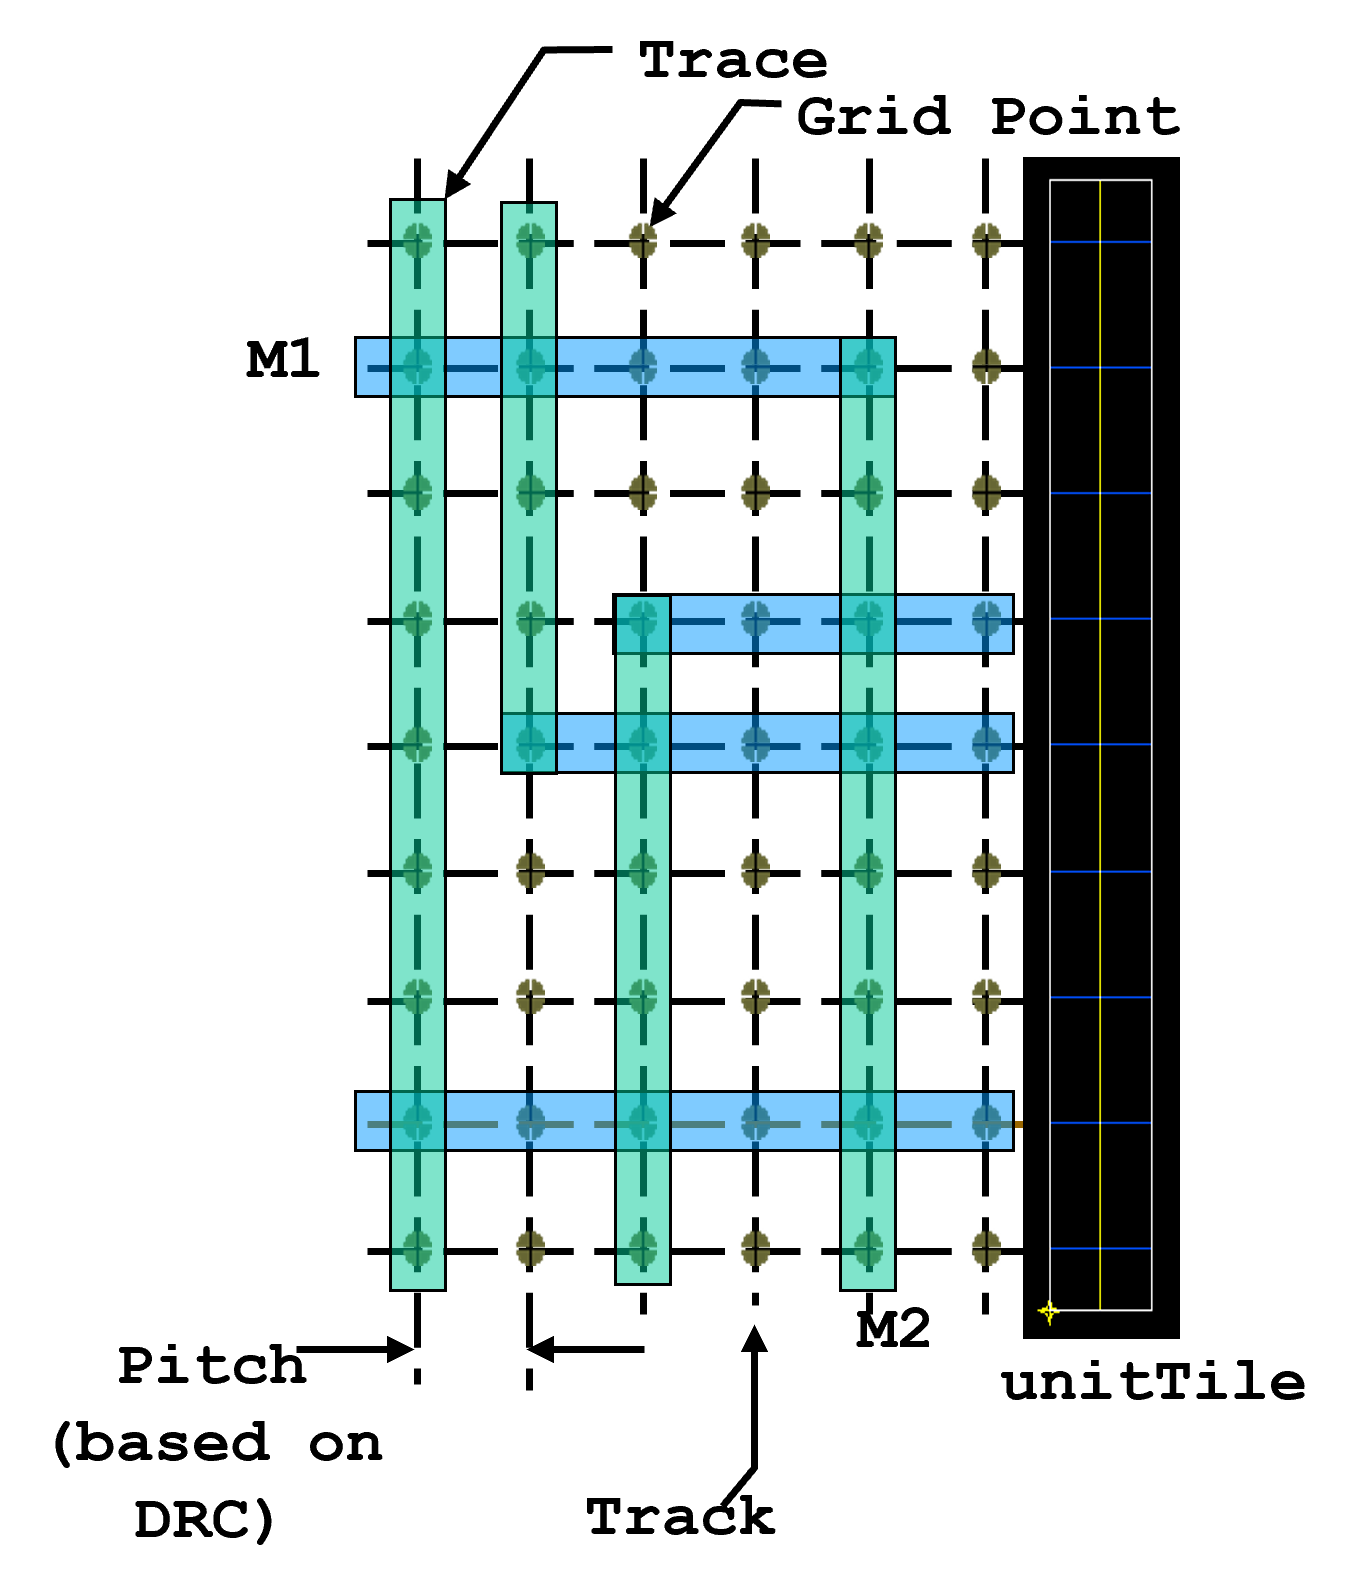
\includegraphics[width=0.8\textwidth]{Grid}
		\end{center}
		\end{columns}	
	\end{frame}
	\begin{frame}
		\frametitle{Peculiarities of Grid-Based Routing System in IC Compiler}
		\begin{itemize}
		\item The "unitTile" shown as a screen shot is used to define and store routing tracks and preferred directions information. 
		\item unitTile cell is part of the standard cell library.
		\item The unitTile is similar to a site. It defines several things:
		\begin{itemize}
			\item The minimum height and width a cell can occupy
			\item The pitches in the preferred direction
			\item Power and ground rail locations for standard cells
			
		\end{itemize}
		\item The height of the unitTile is based on the metal 1 pitch (vertical) and must be a multiple of it. 
		\item The width is based on the metal 2 pitch (horizontal) and must be a multiple of it.
	\item The metal 2 routing track defined in it must either be along the left side boundary or centered in the unitTile. 
		
		\end{itemize}
	\end{frame}
%----------------------------------
\section[Routing]{Routing Operations}
\subsection[Operations]{Routing Operations}	
	\begin{frame}
		\frametitle{Routing Operations}
		\begin{columns}	
			\column{0.5\textwidth}
			\begin{itemize}
				\item \textbf{PnR Compiler performs:}
				\begin{enumerate}
					\item Global Routing
					\item Track Assignment
					\item Detail Routing
					\item Search and Repair
				\end{enumerate}
			\end{itemize}
			\column{0.5\textwidth}
			\begin{center}
				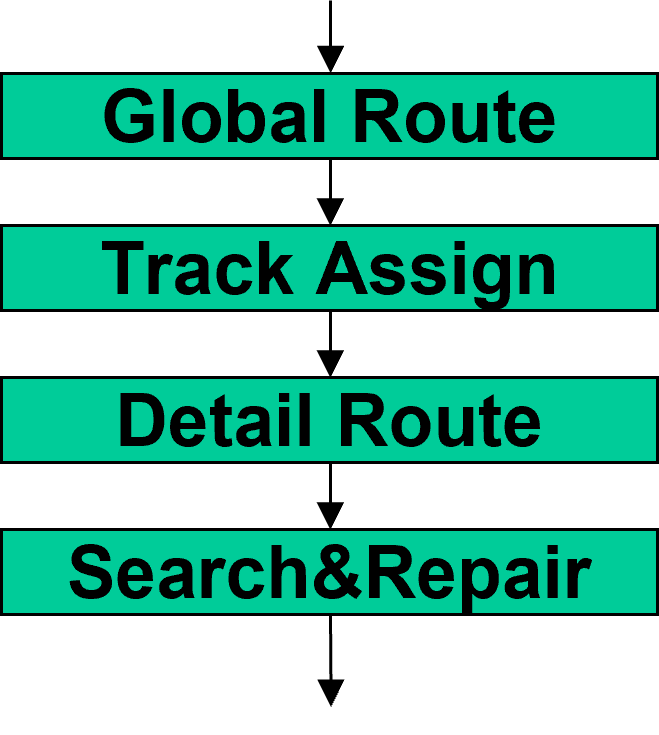
\includegraphics[width=0.5\textwidth]{operation}
			\end{center}
		\end{columns}
\begin{itemize}
	\item \textbf{After global routing, track assignment and detail routing all clock/signal nets will be completely routed and should meet all timing, and most all DRC, requirements}
	\item \textbf{Any remaining DRC violations can be fixed by Search \& Repair}
\end{itemize}
\end{frame}	
\subsection[Global]{Global Route}
\begin{frame}
	\frametitle{Route Operations: Global Route}
	\begin{itemize}
		\item \textbf{Global Route (GR) is the first step in routing}
		\item \textbf{GR gives more accurate parasitic and delay estimates compared to VR.}
		\item \textbf{The Global Route that is performed during routing will be used by the subsequent Track Assign operation}
		\item \textcolor{red}{Determining overall path of all routes}
		\item \textcolor{red}{Seeking to reduce delay, channel widths}
	\end{itemize}
	\begin{center}
		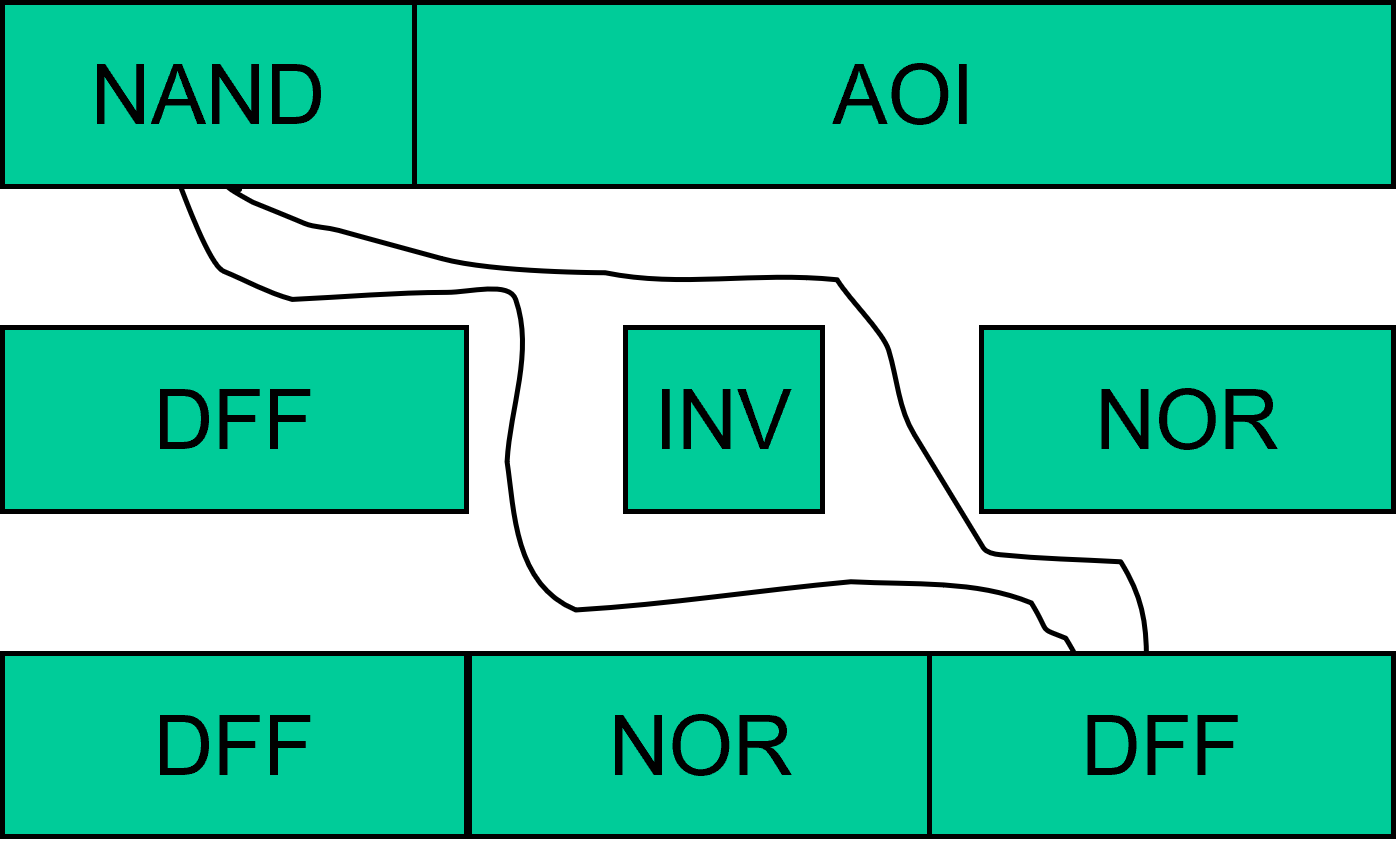
\includegraphics[width=0.5\textwidth]{GLOBAL}
	\end{center}
\end{frame}

\begin{frame}
	\frametitle{Route Operations: Global Route}
	\begin{center}
		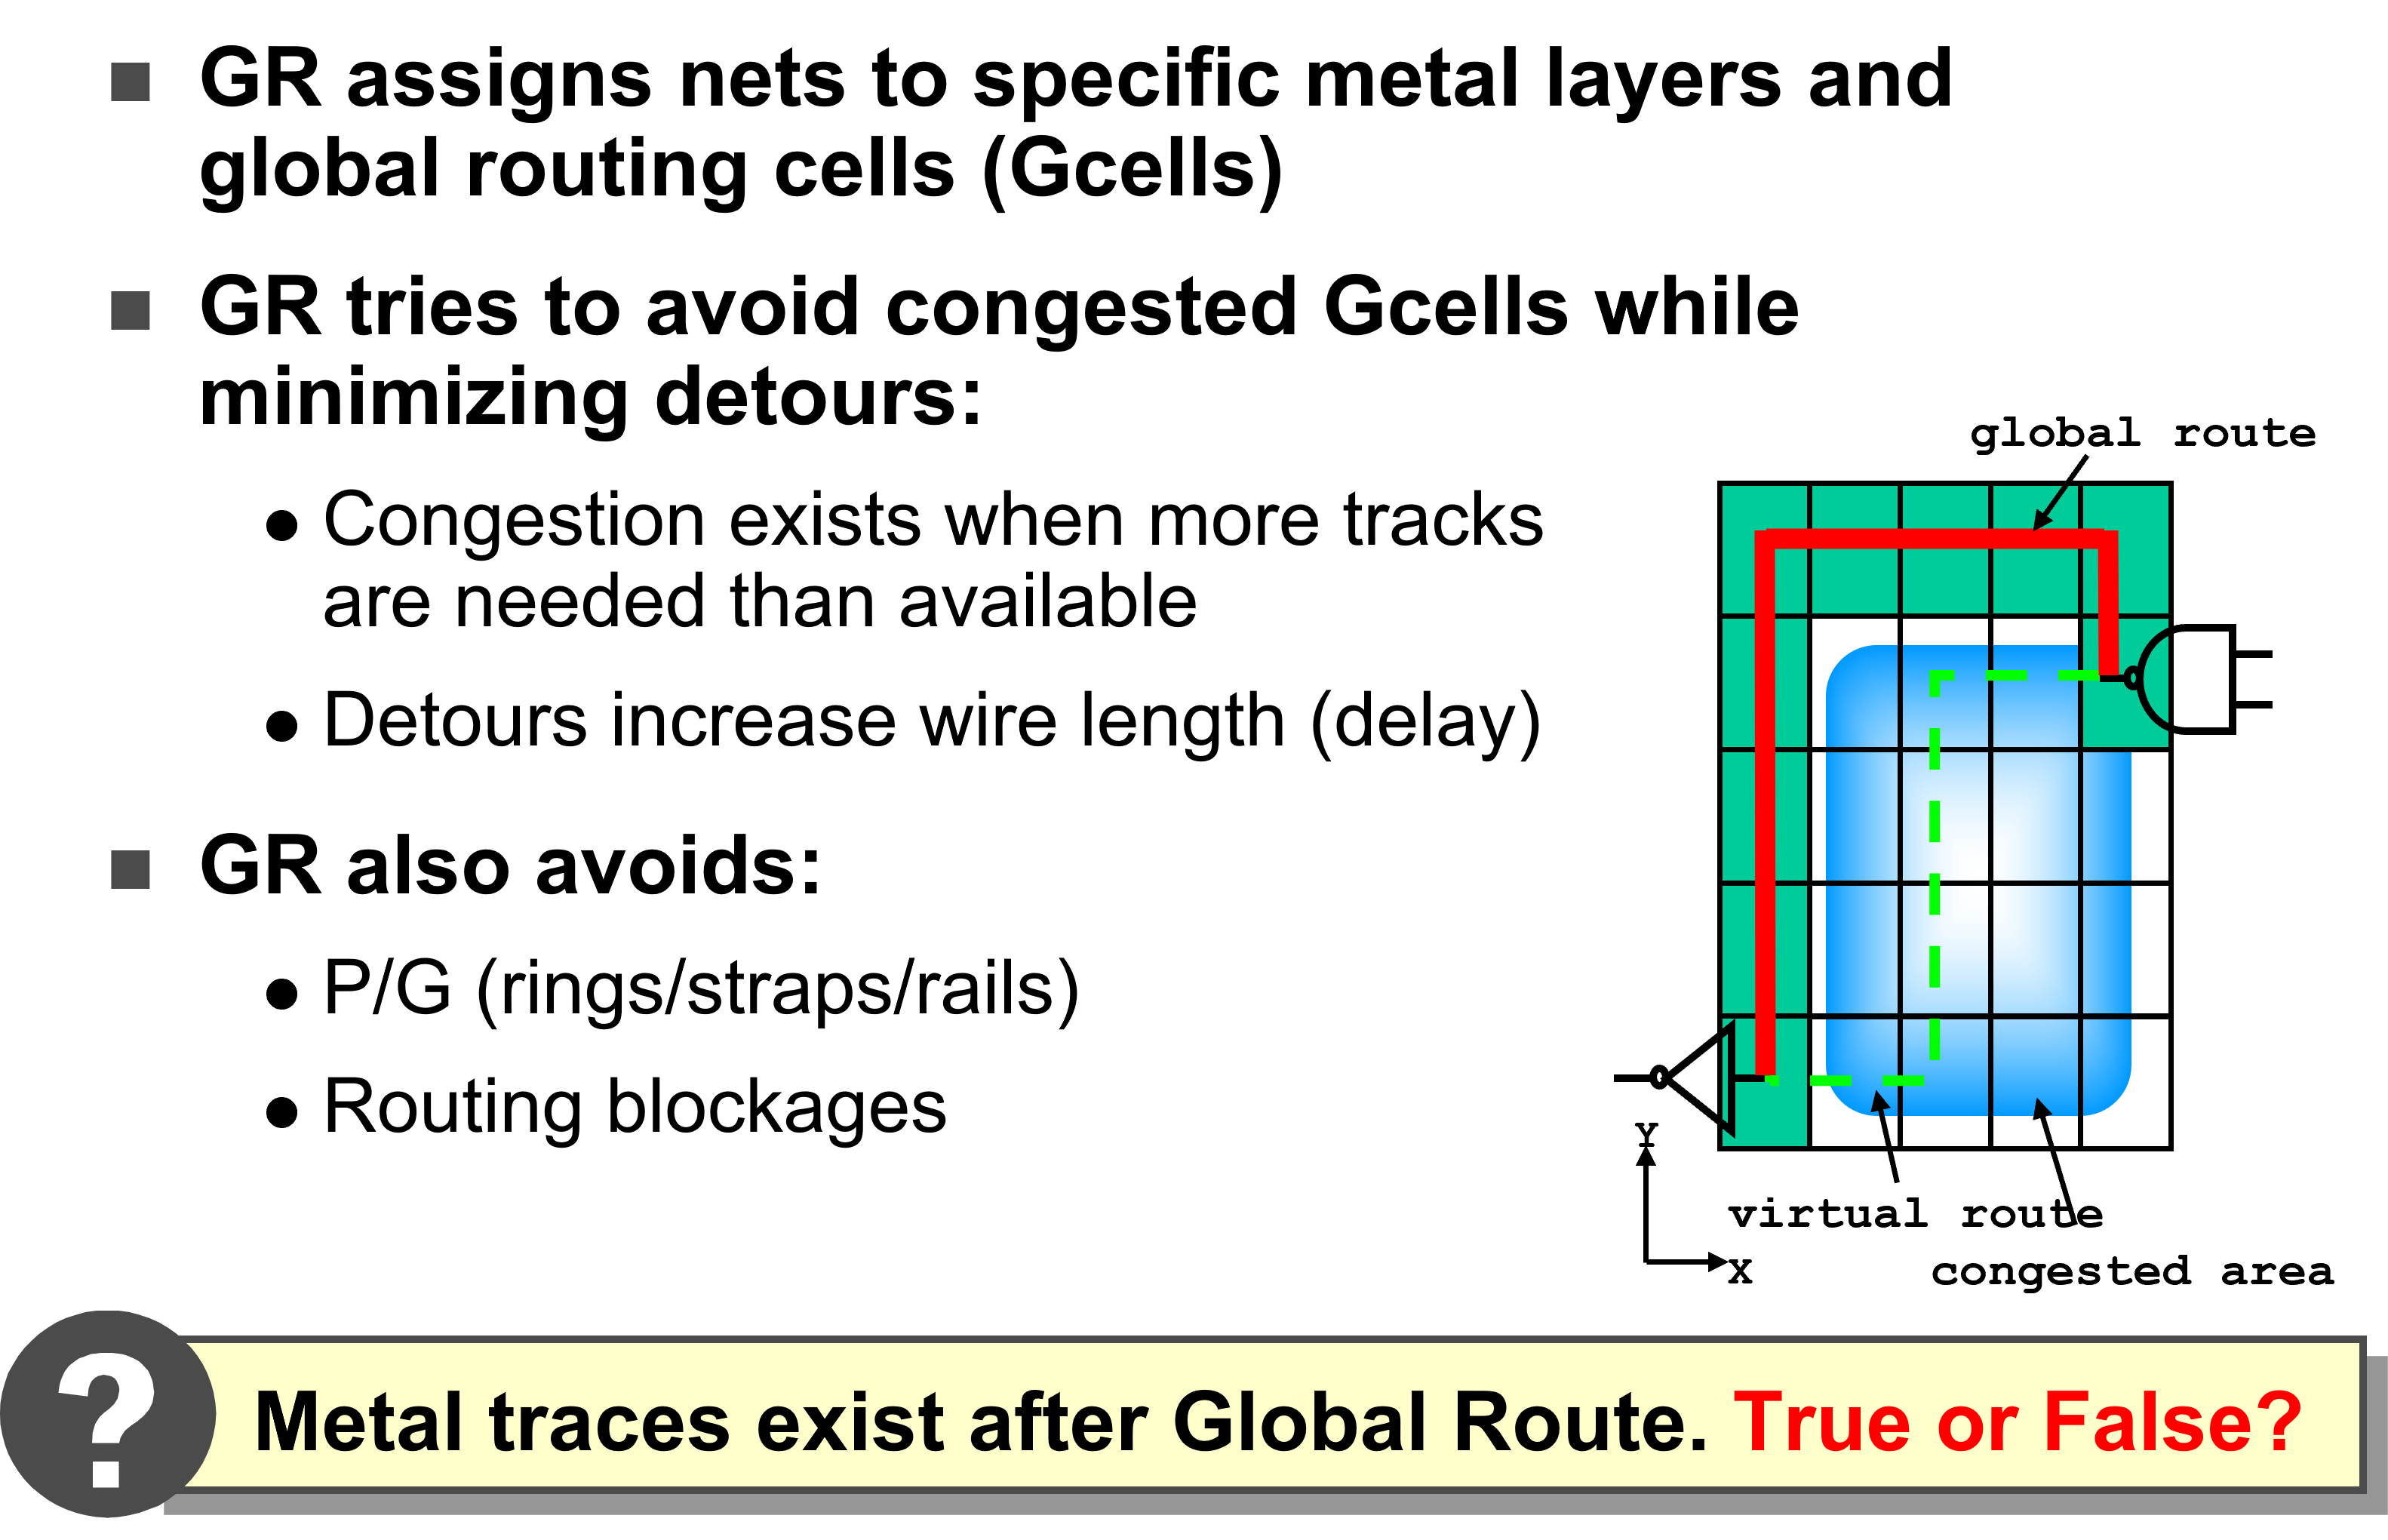
\includegraphics[width=\textwidth]{groute}
	\end{center}

\end{frame}
\begin{frame}
	\frametitle{Route Operations: Global Route Summary}
	\begin{columns}
		\column{0.3\textwidth}
		\textbf{Answer: False!} \newline
		\textbf{GR does not lay down any metal traces.}
		\column{0.7\textwidth}
			\begin{center}
			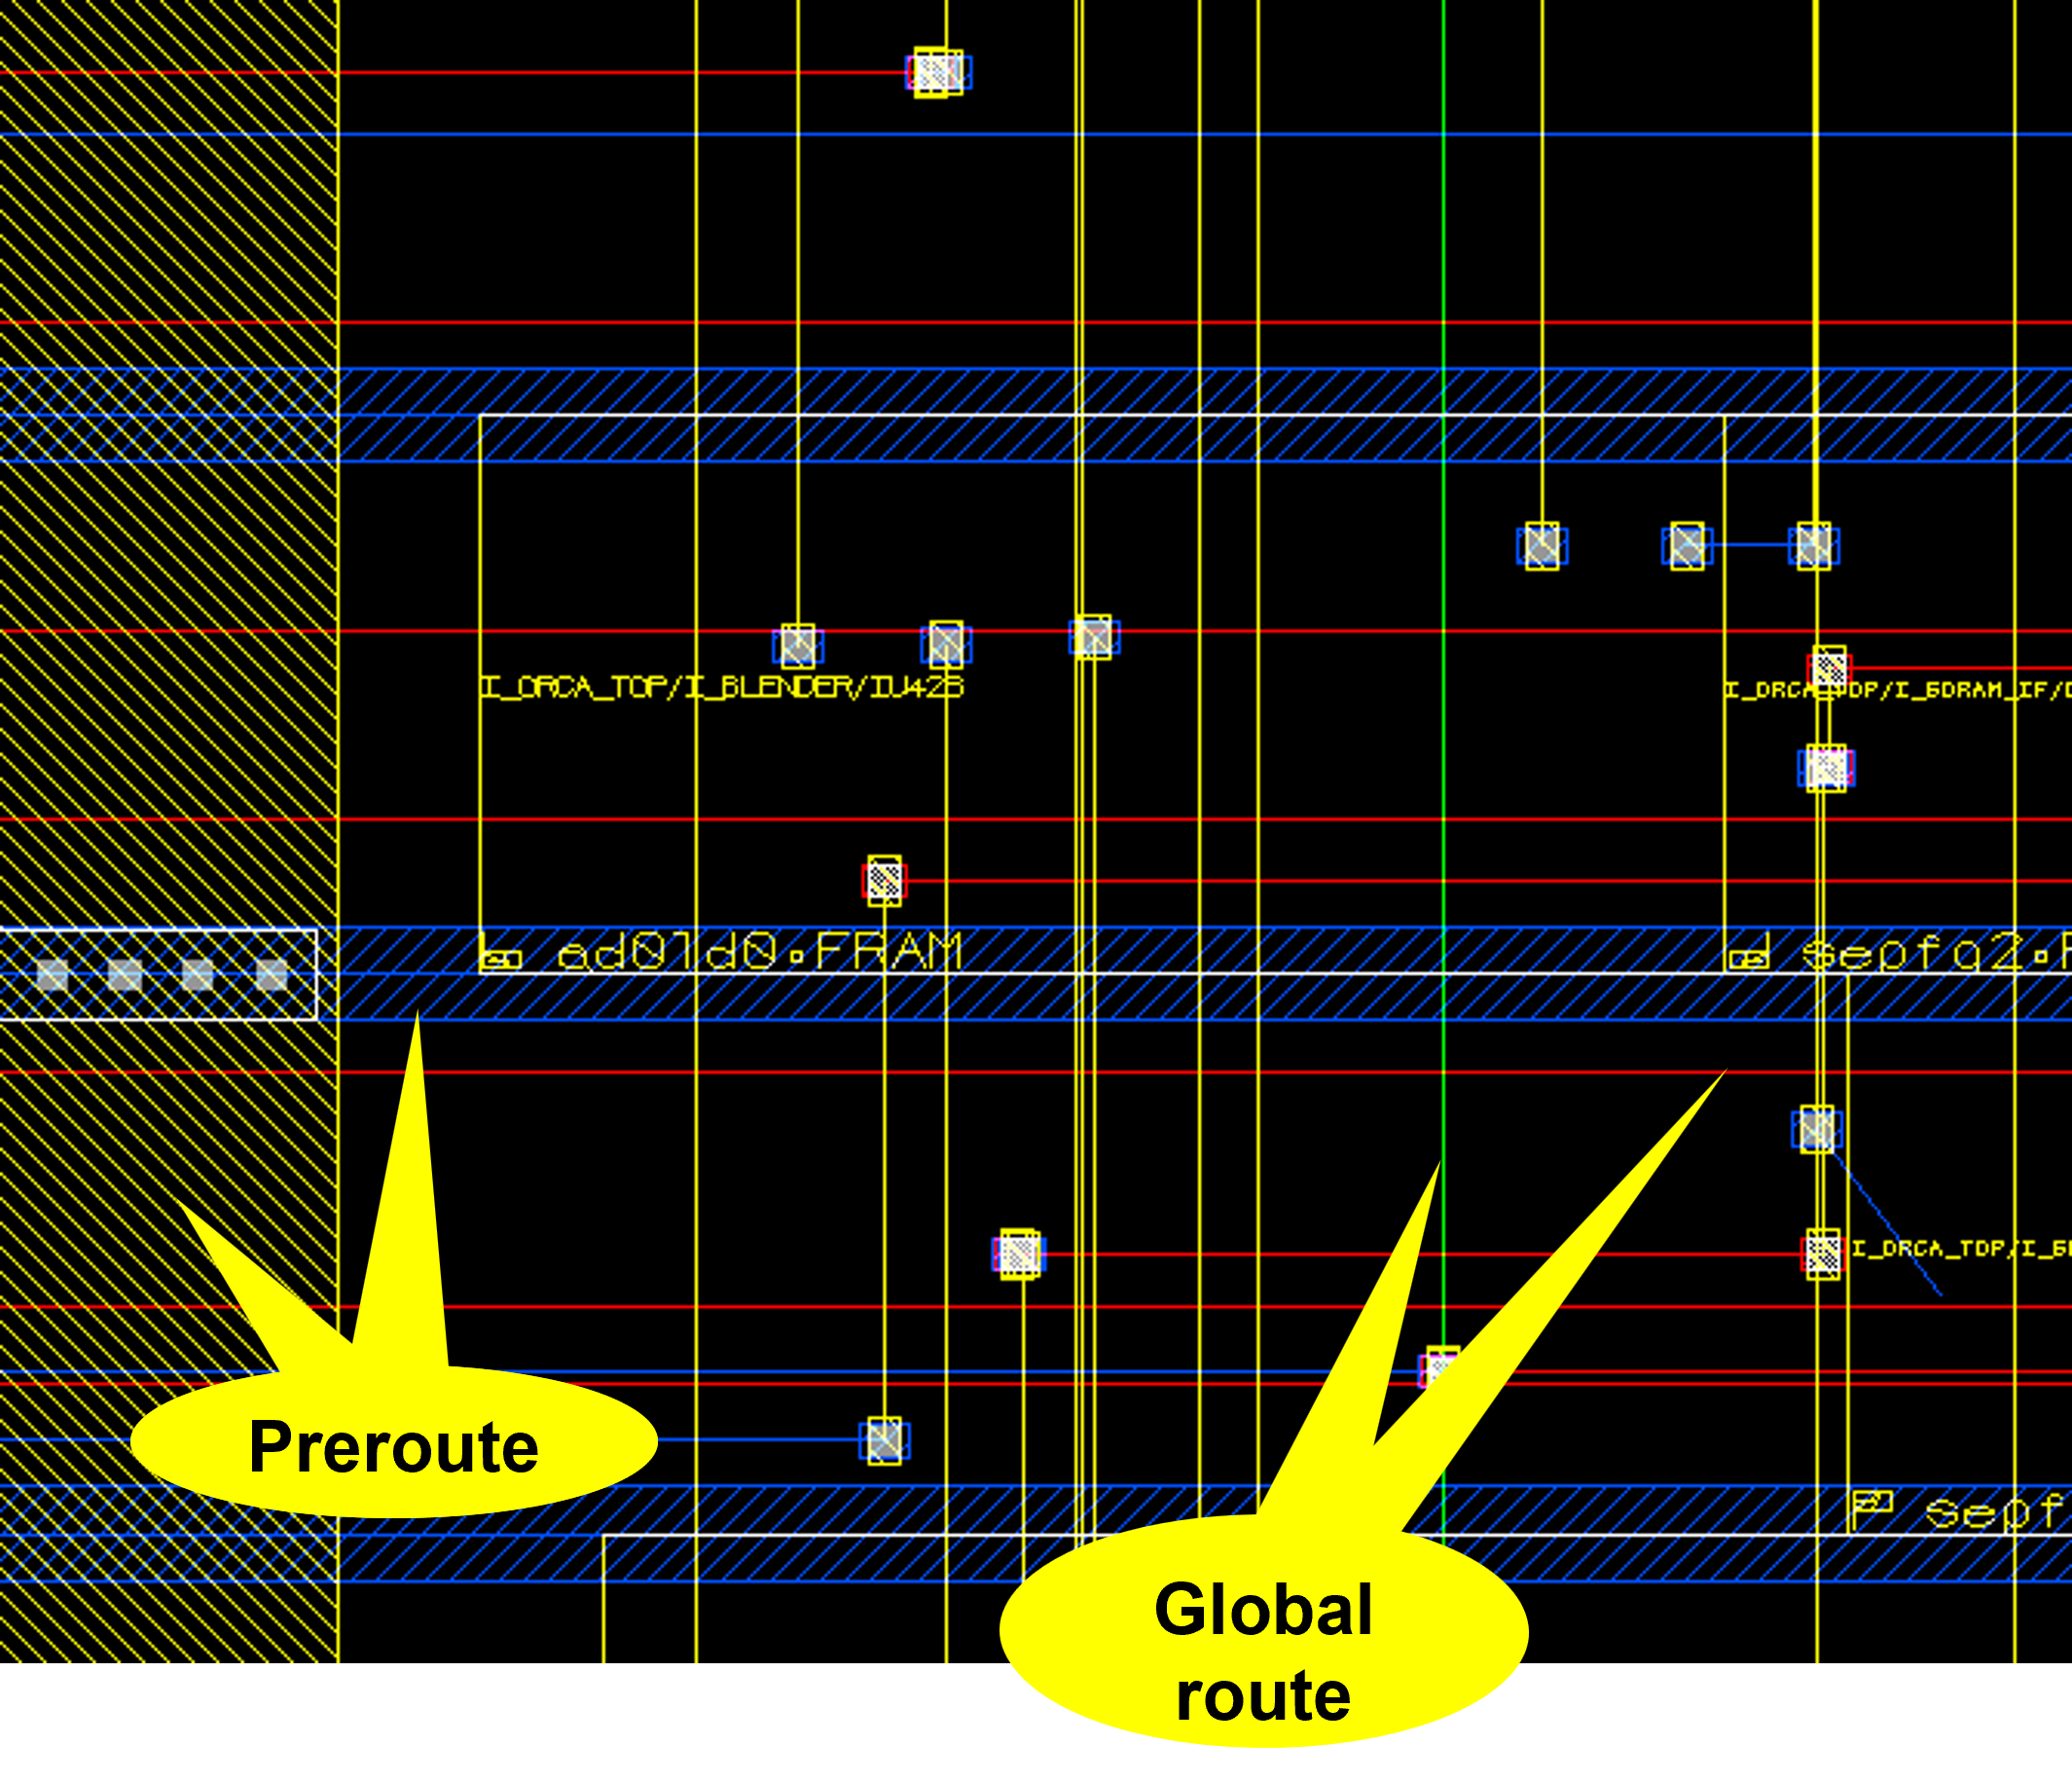
\includegraphics[width=\textwidth]{groute2}
		\end{center}
	\end{columns}
\end{frame}

\subsection[Track]{Track Assignment}
\begin{frame}
	\frametitle{Route Operations: Track Assignment}
	\begin{center}
		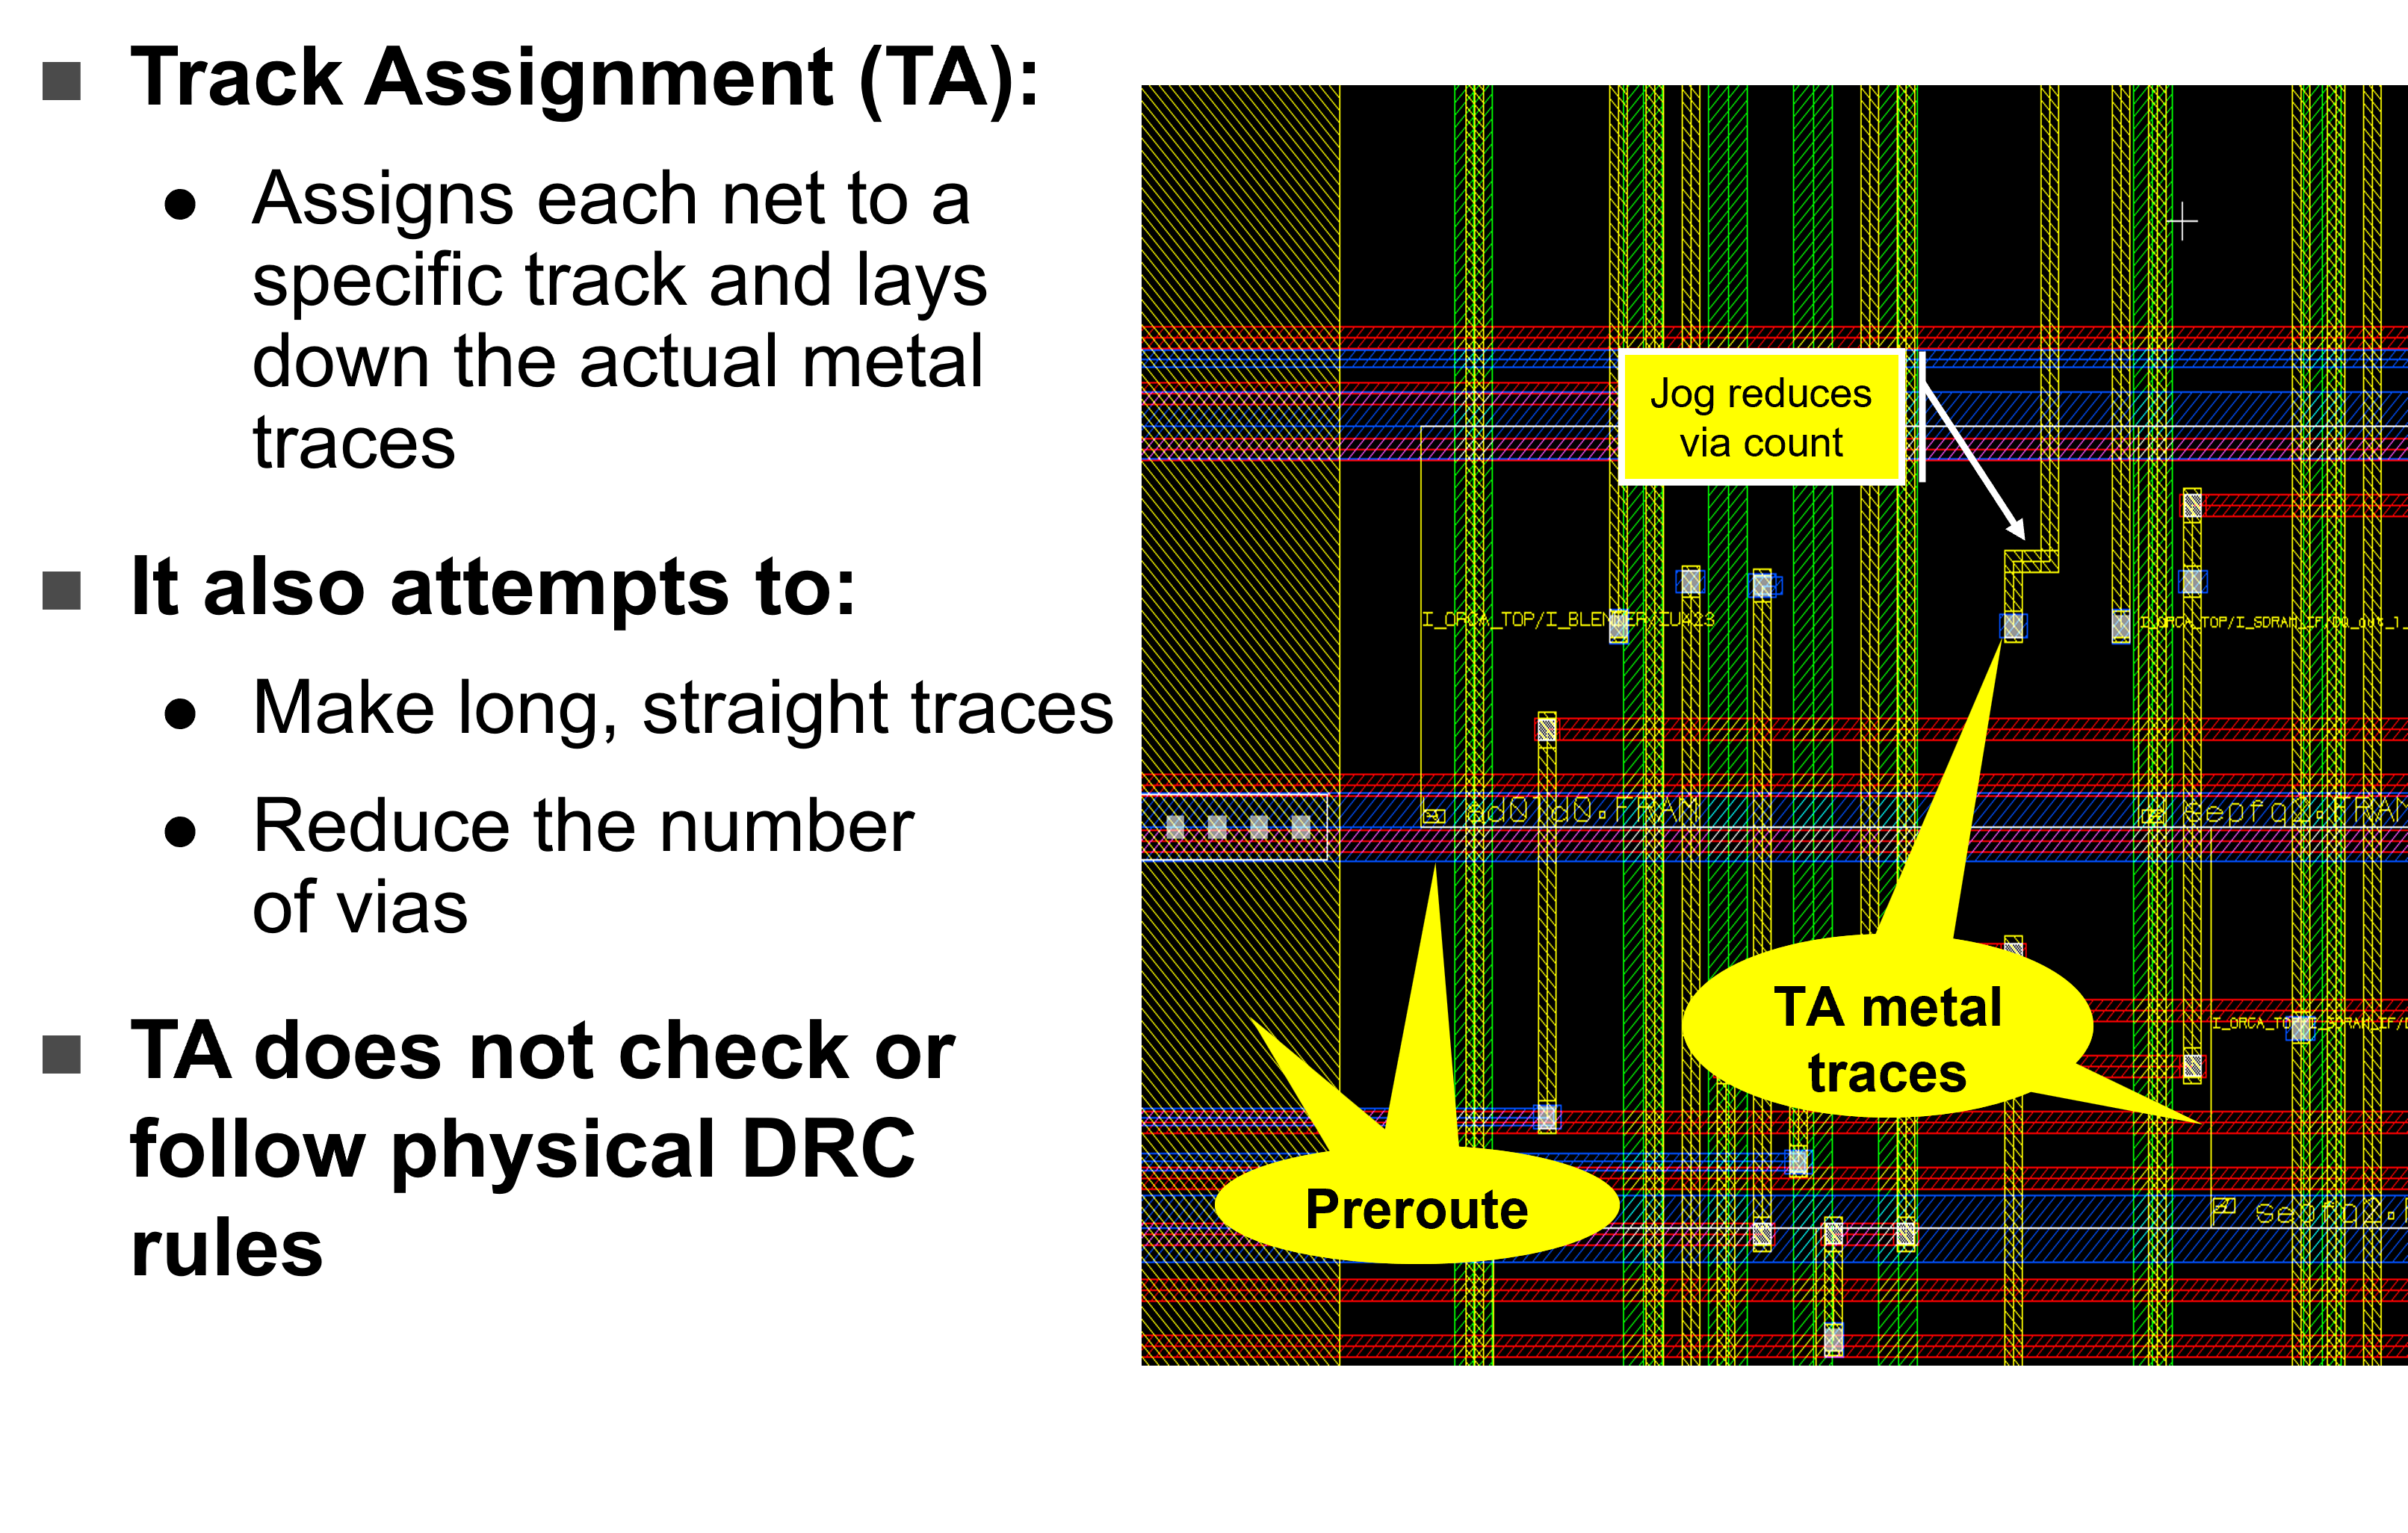
\includegraphics[width=\textwidth]{TRACK}
	\end{center}
\end{frame}	
\subsection[Detail]{Detail Routing}
\begin{frame}
	\frametitle{Route Operations: Detail Routing}
	\begin{itemize}
		\item \textbf{Detail route attempts to clear DRC violations using a fixed size Sbox}
		\begin{center}
			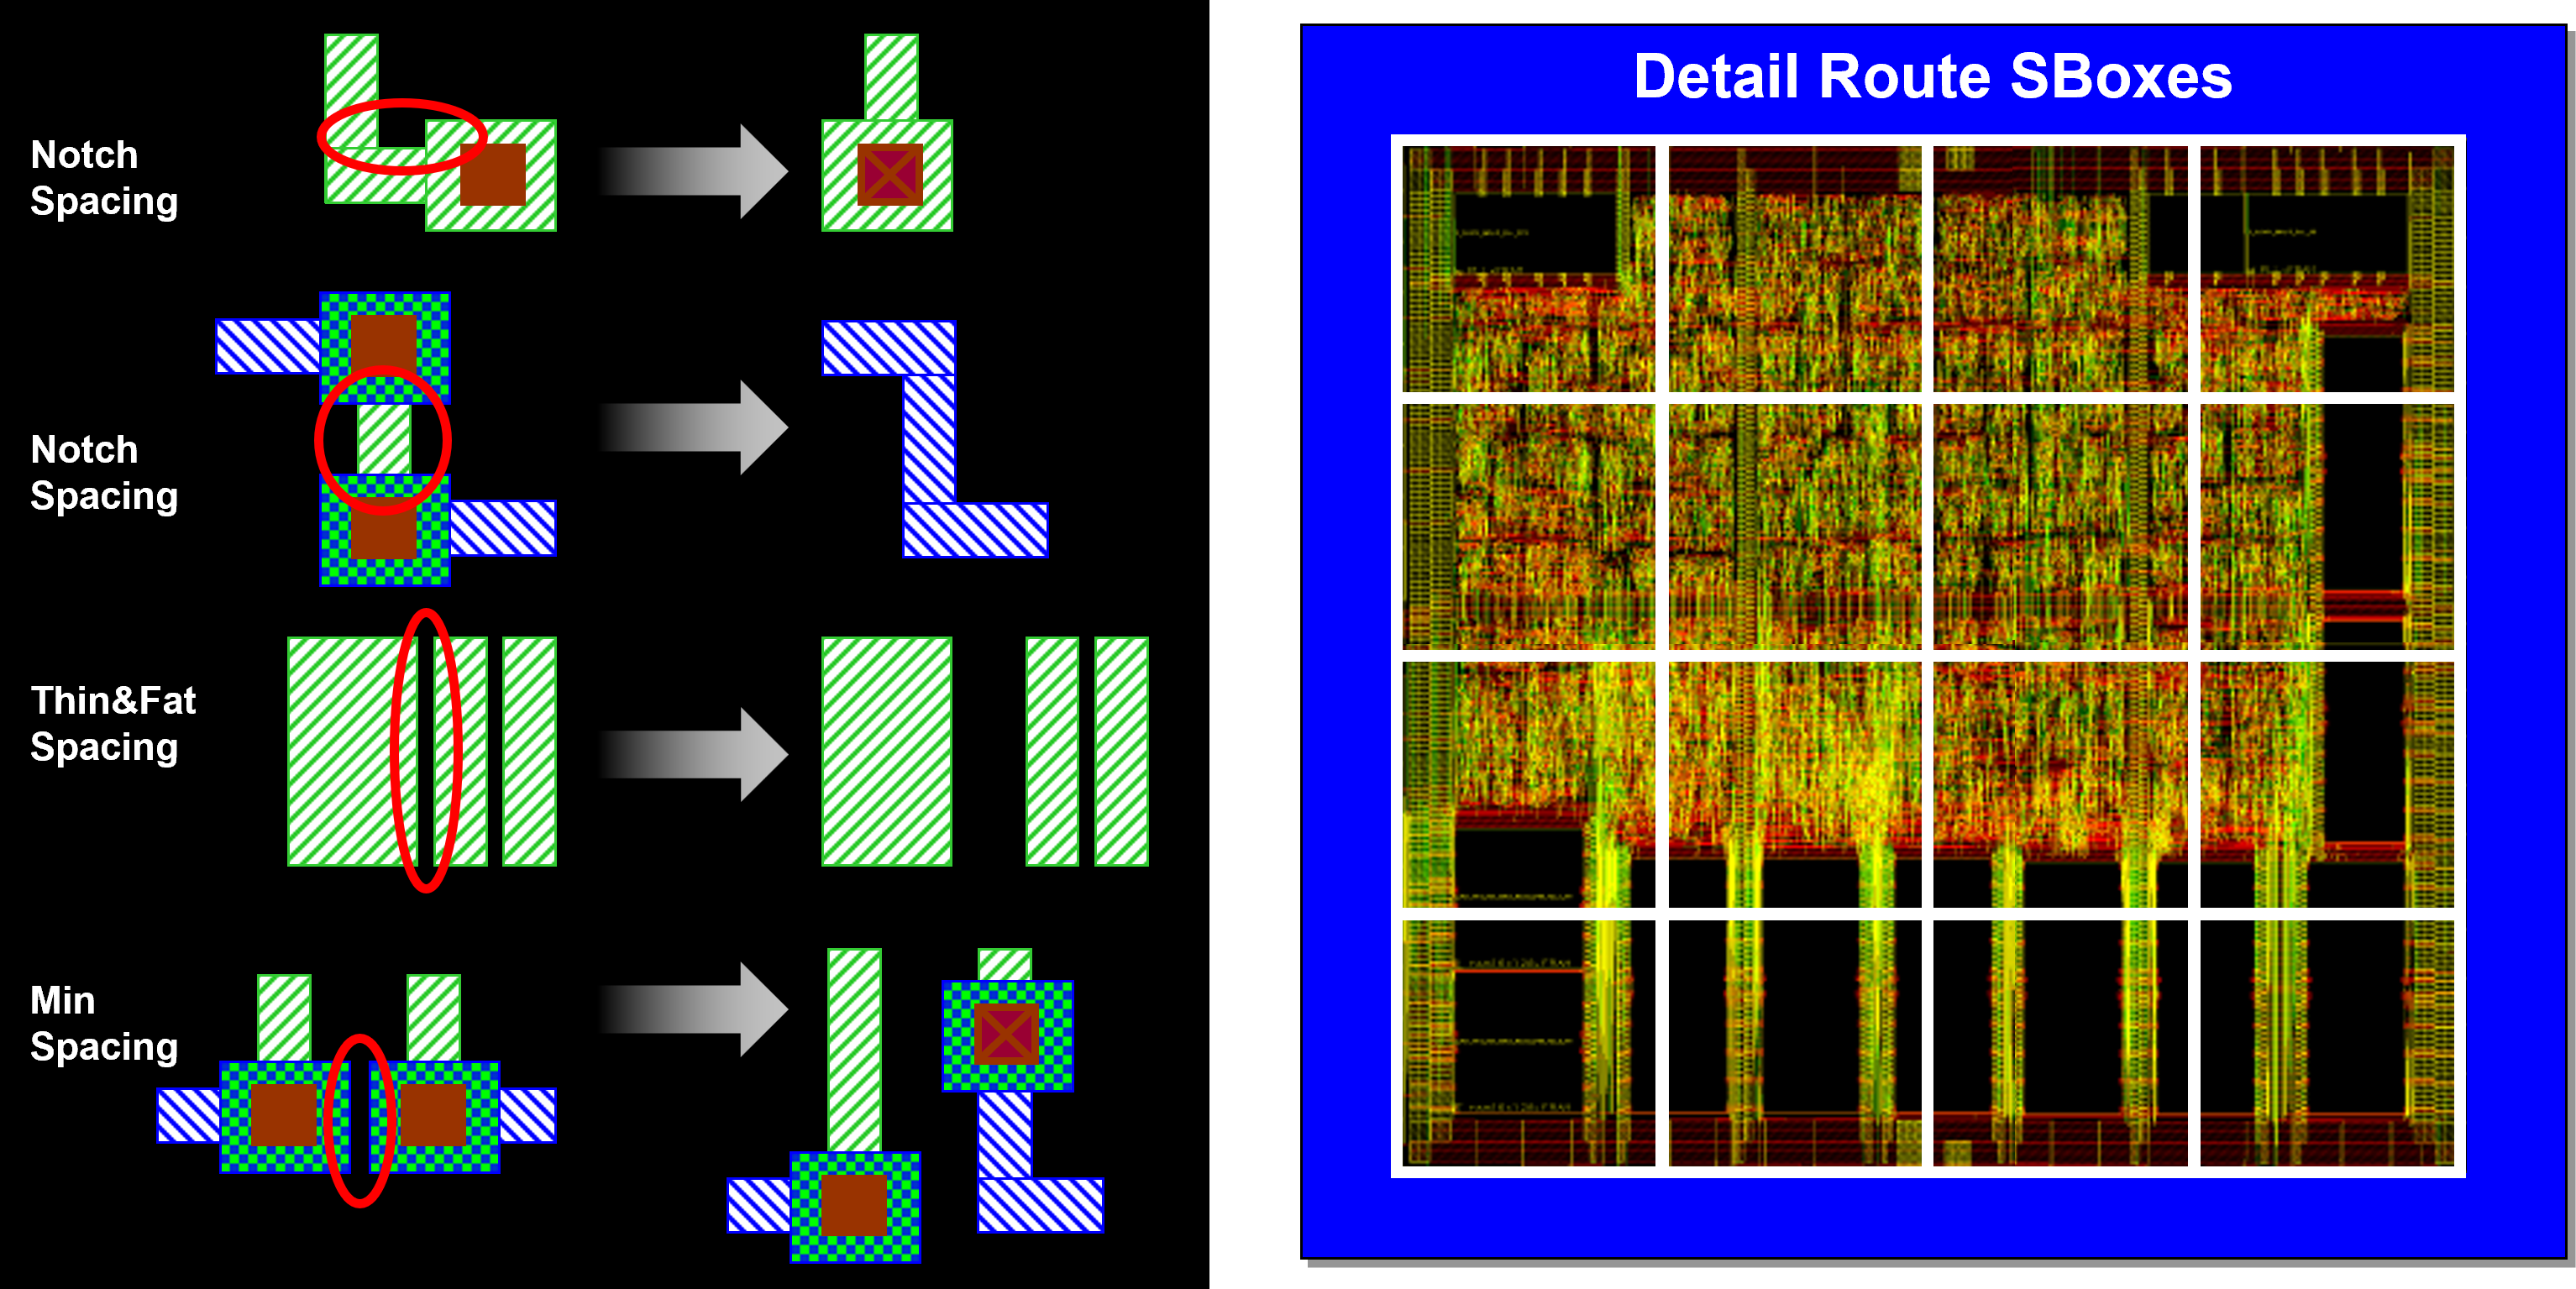
\includegraphics[width=0.9\textwidth]{Detail}
		\end{center}
	\item \textbf{Due to the fixed Sbox size, detail route may not be able to clear all DRC violations}	
	\end{itemize}
\end{frame}
\subsection[S\&R]{Search\&Repair}
\begin{frame}
	\frametitle{Route Operations: Search\&Repair}
	\begin{itemize}
		\item \textbf{Search\&Repair fixes remaining DRC violations through multiple loops using progressively larger SBox sizes}
		\begin{center}
			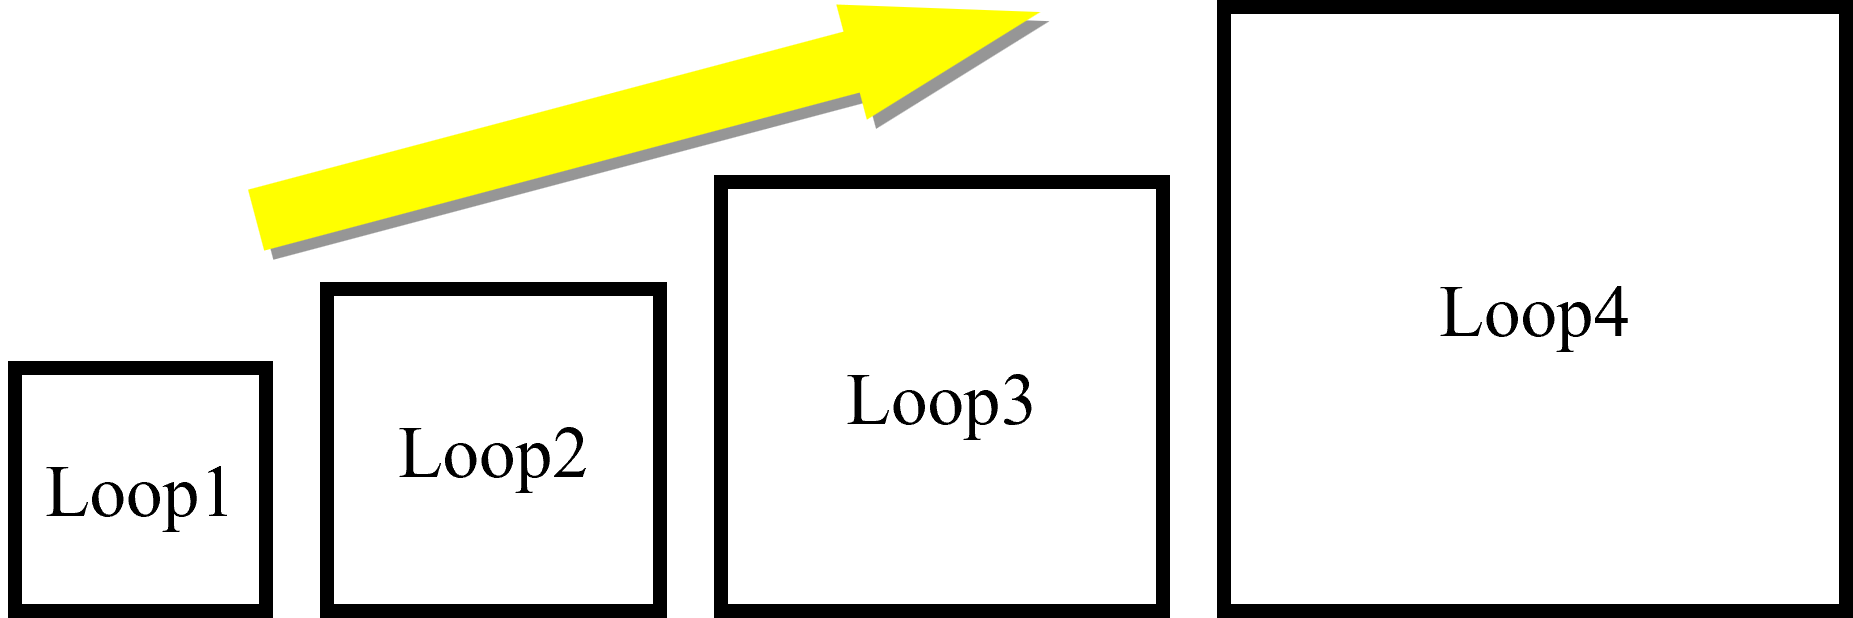
\includegraphics[width=0.7\textwidth]{SR}
		\end{center}
	\item \textbf{Note: Even if the design is DRC clean after S\&R, you must still run a sign-off DRC checker (Caliber).}
	\begin{itemize}
		\item Routing DRC rules are a subset of the complete technology DRC rules
		\item IC Compiler works on the FRAM view, not the detailed transistor-level (CEL) view
	\end{itemize}
	\end{itemize}
\end{frame}	

\begin{frame}
	\frametitle{Routing over Macros}
	\begin{center}
		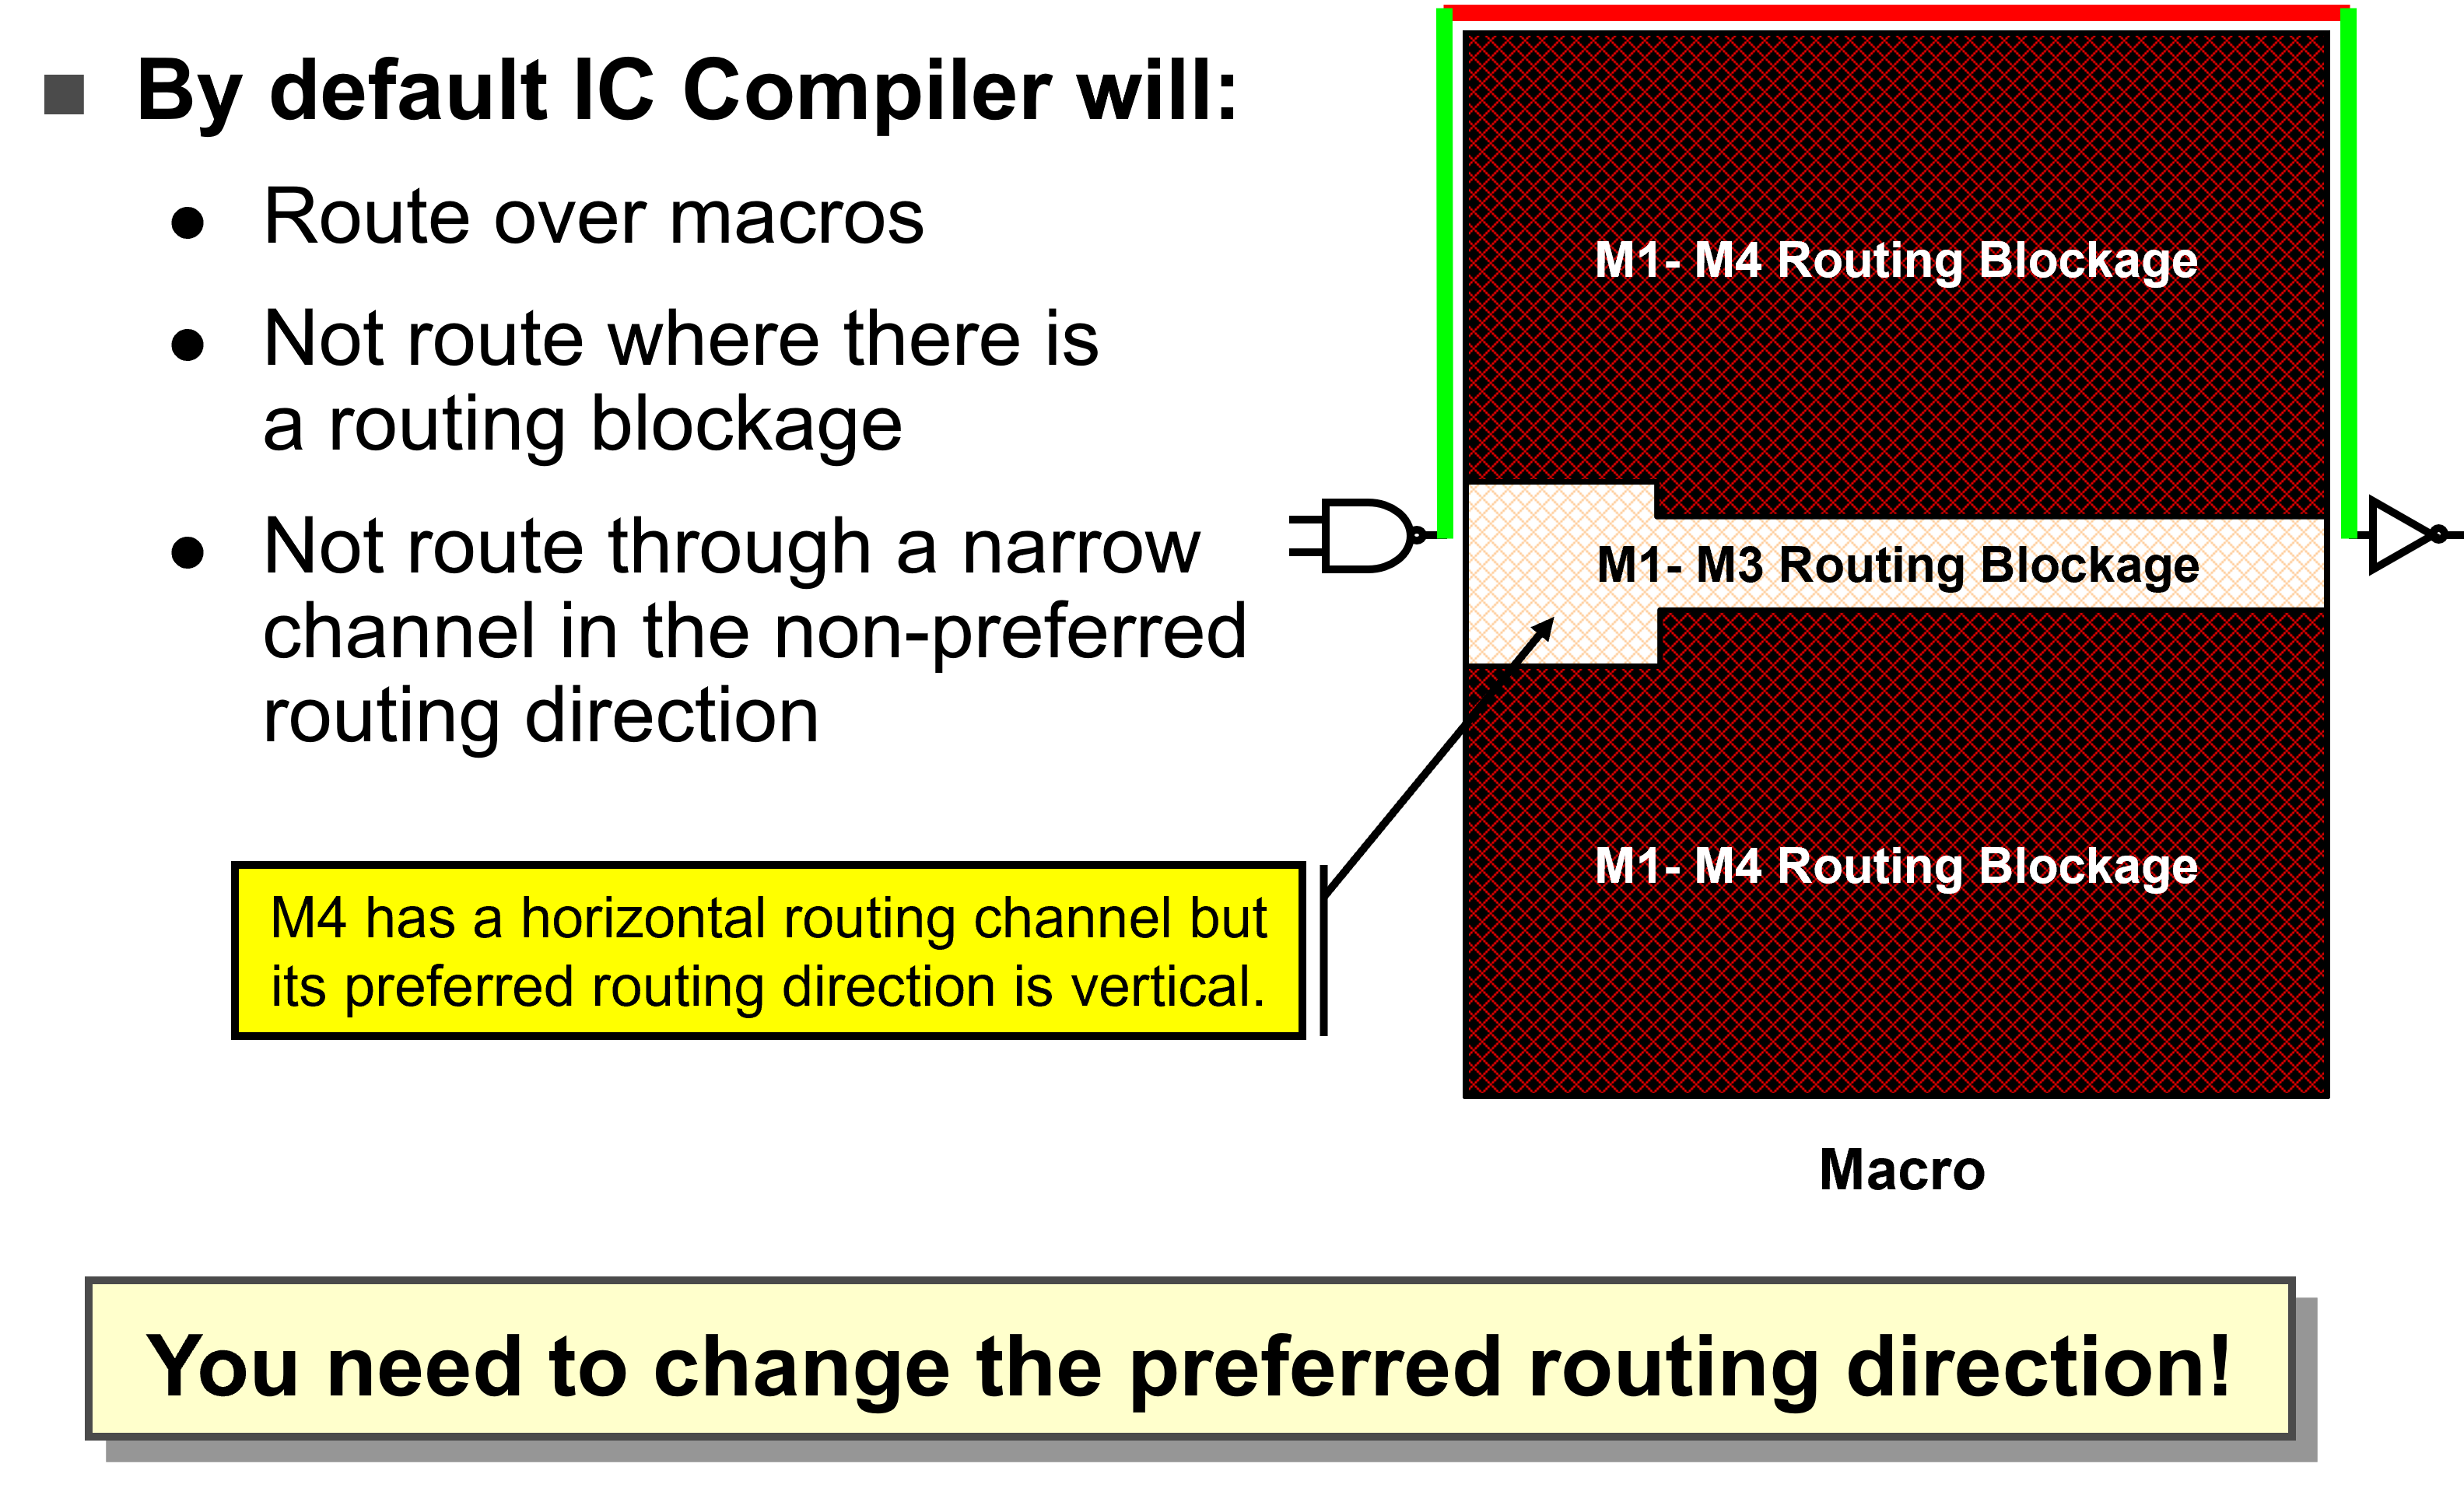
\includegraphics[width=\textwidth]{ro}
	\end{center}
\end{frame}

\section[Crosstalk]{Crosstalk}
\subsection[Crosstalk]{Crosstalk}
\begin{frame}
	\frametitle{What is Crosstalk?}
	\begin{center}
		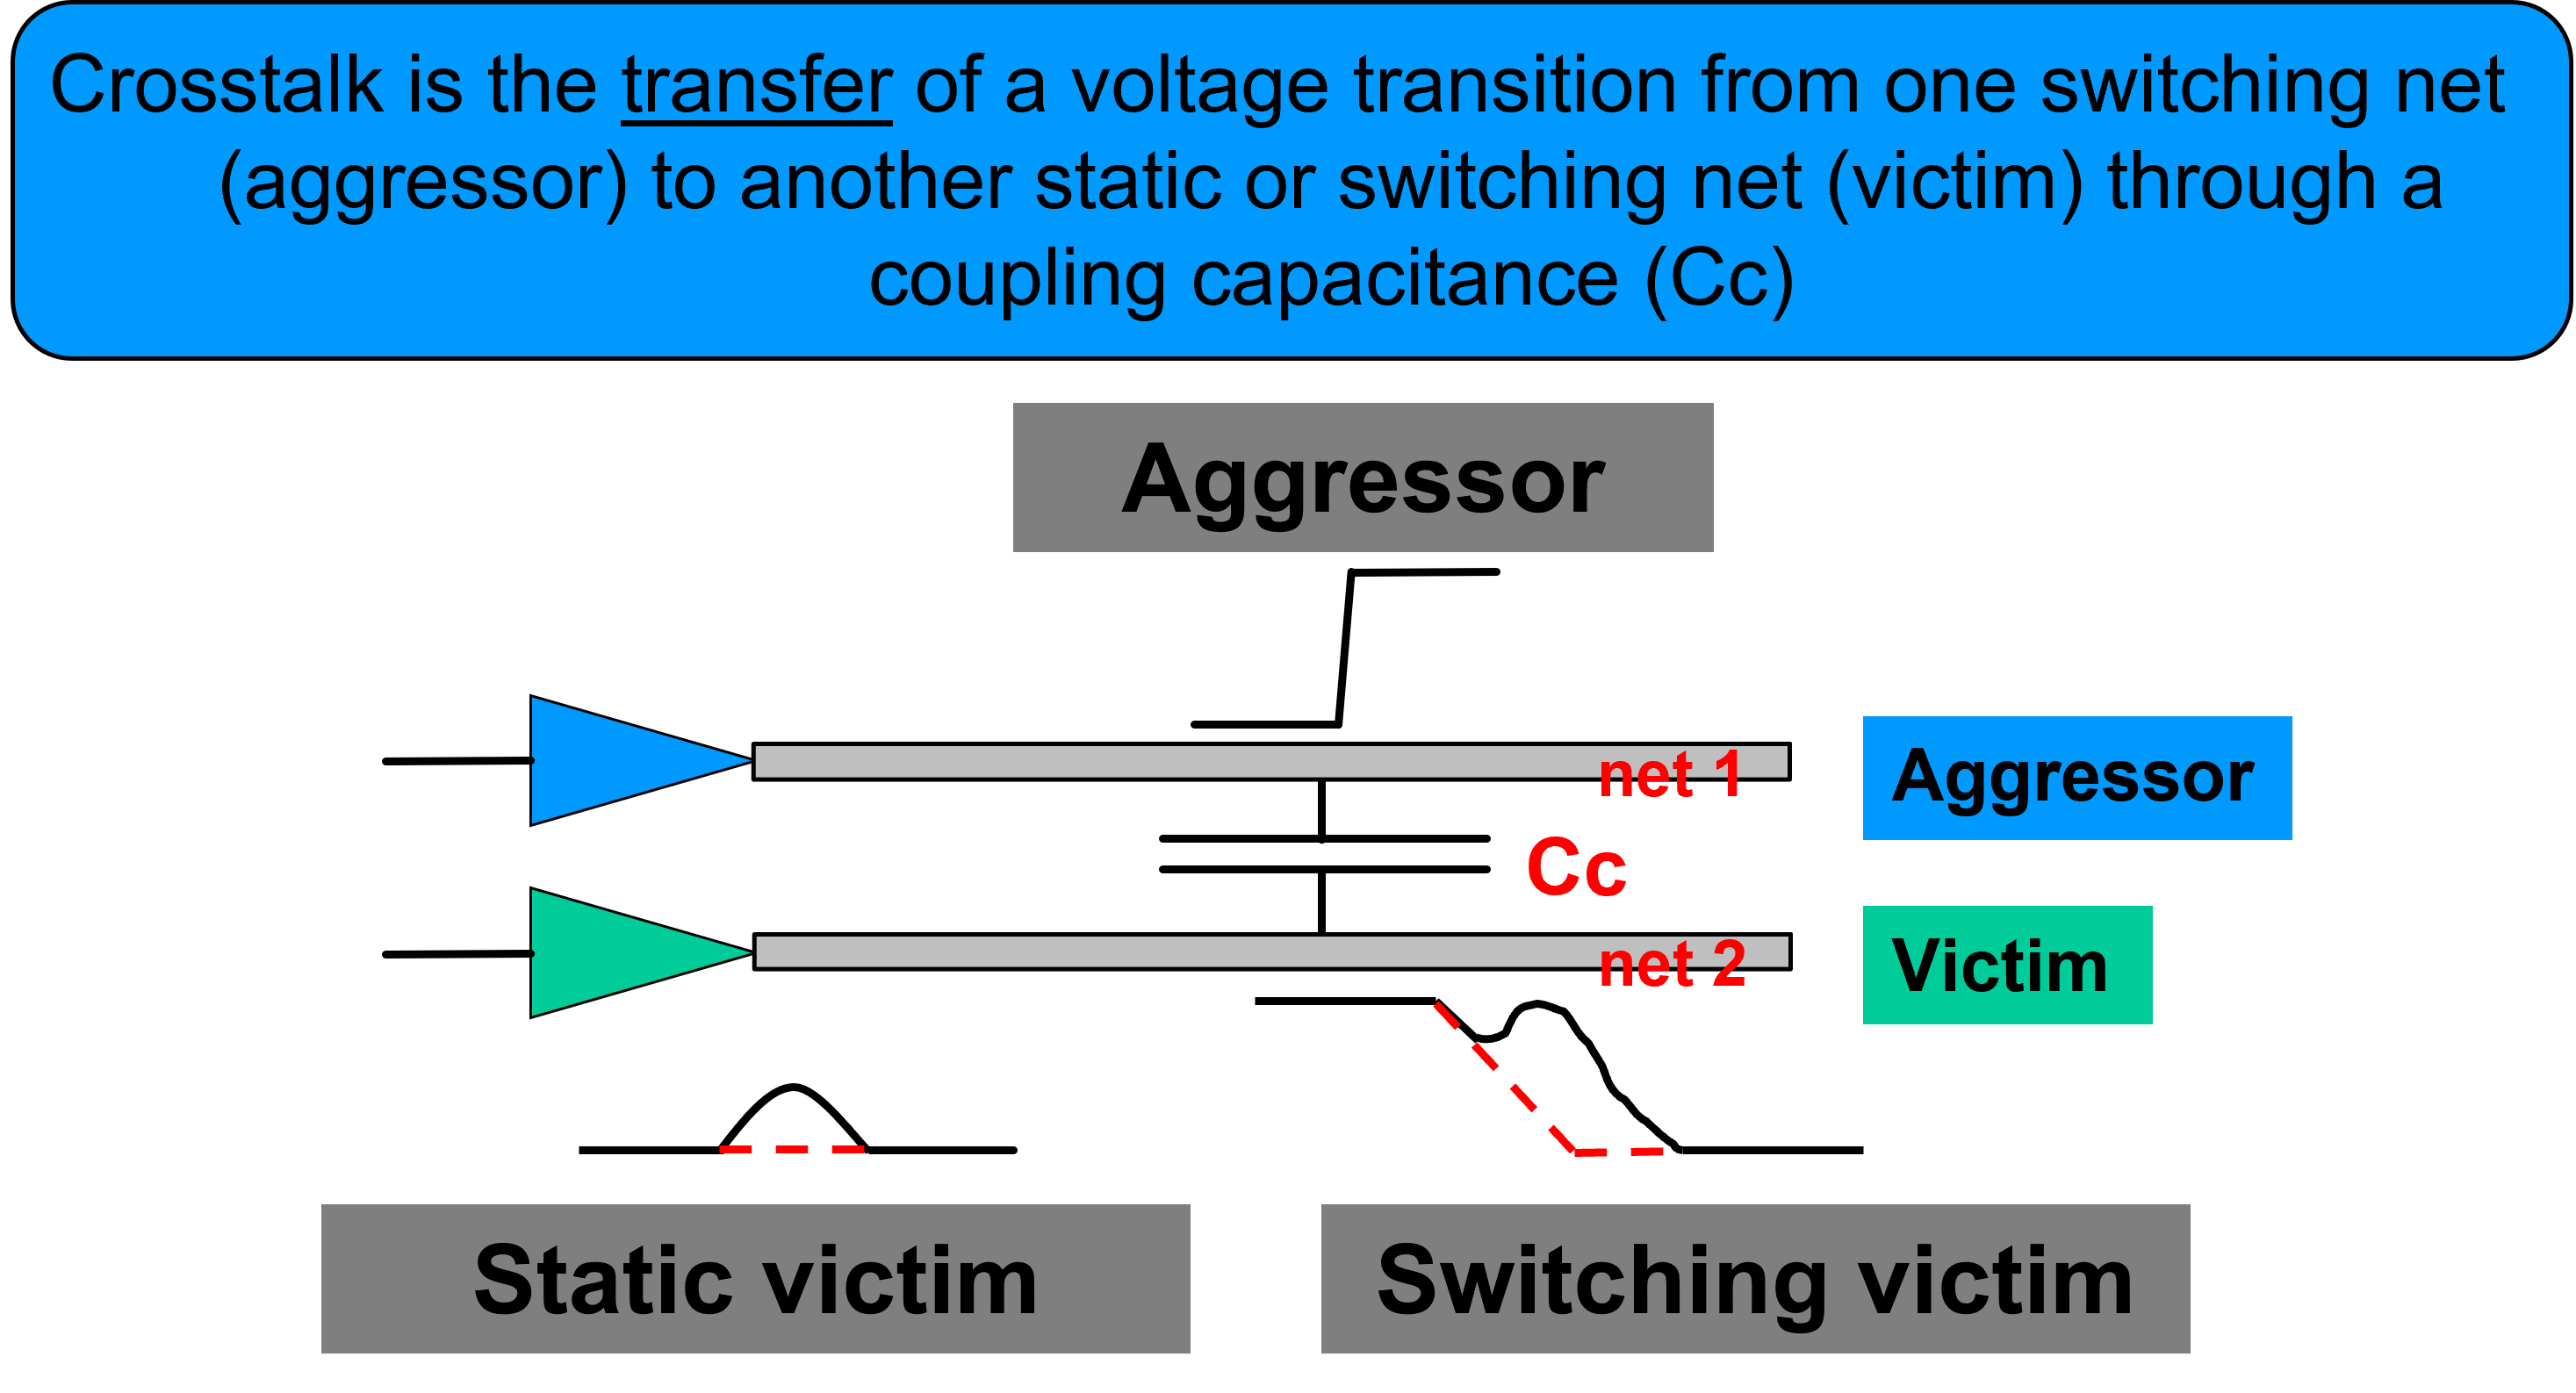
\includegraphics[width=\textwidth]{Crosstalk}
	\end{center}
\end{frame}


\begin{frame}
	\frametitle{Crosstalk-Induced Noise (aka Glitches)}
	\begin{center}
		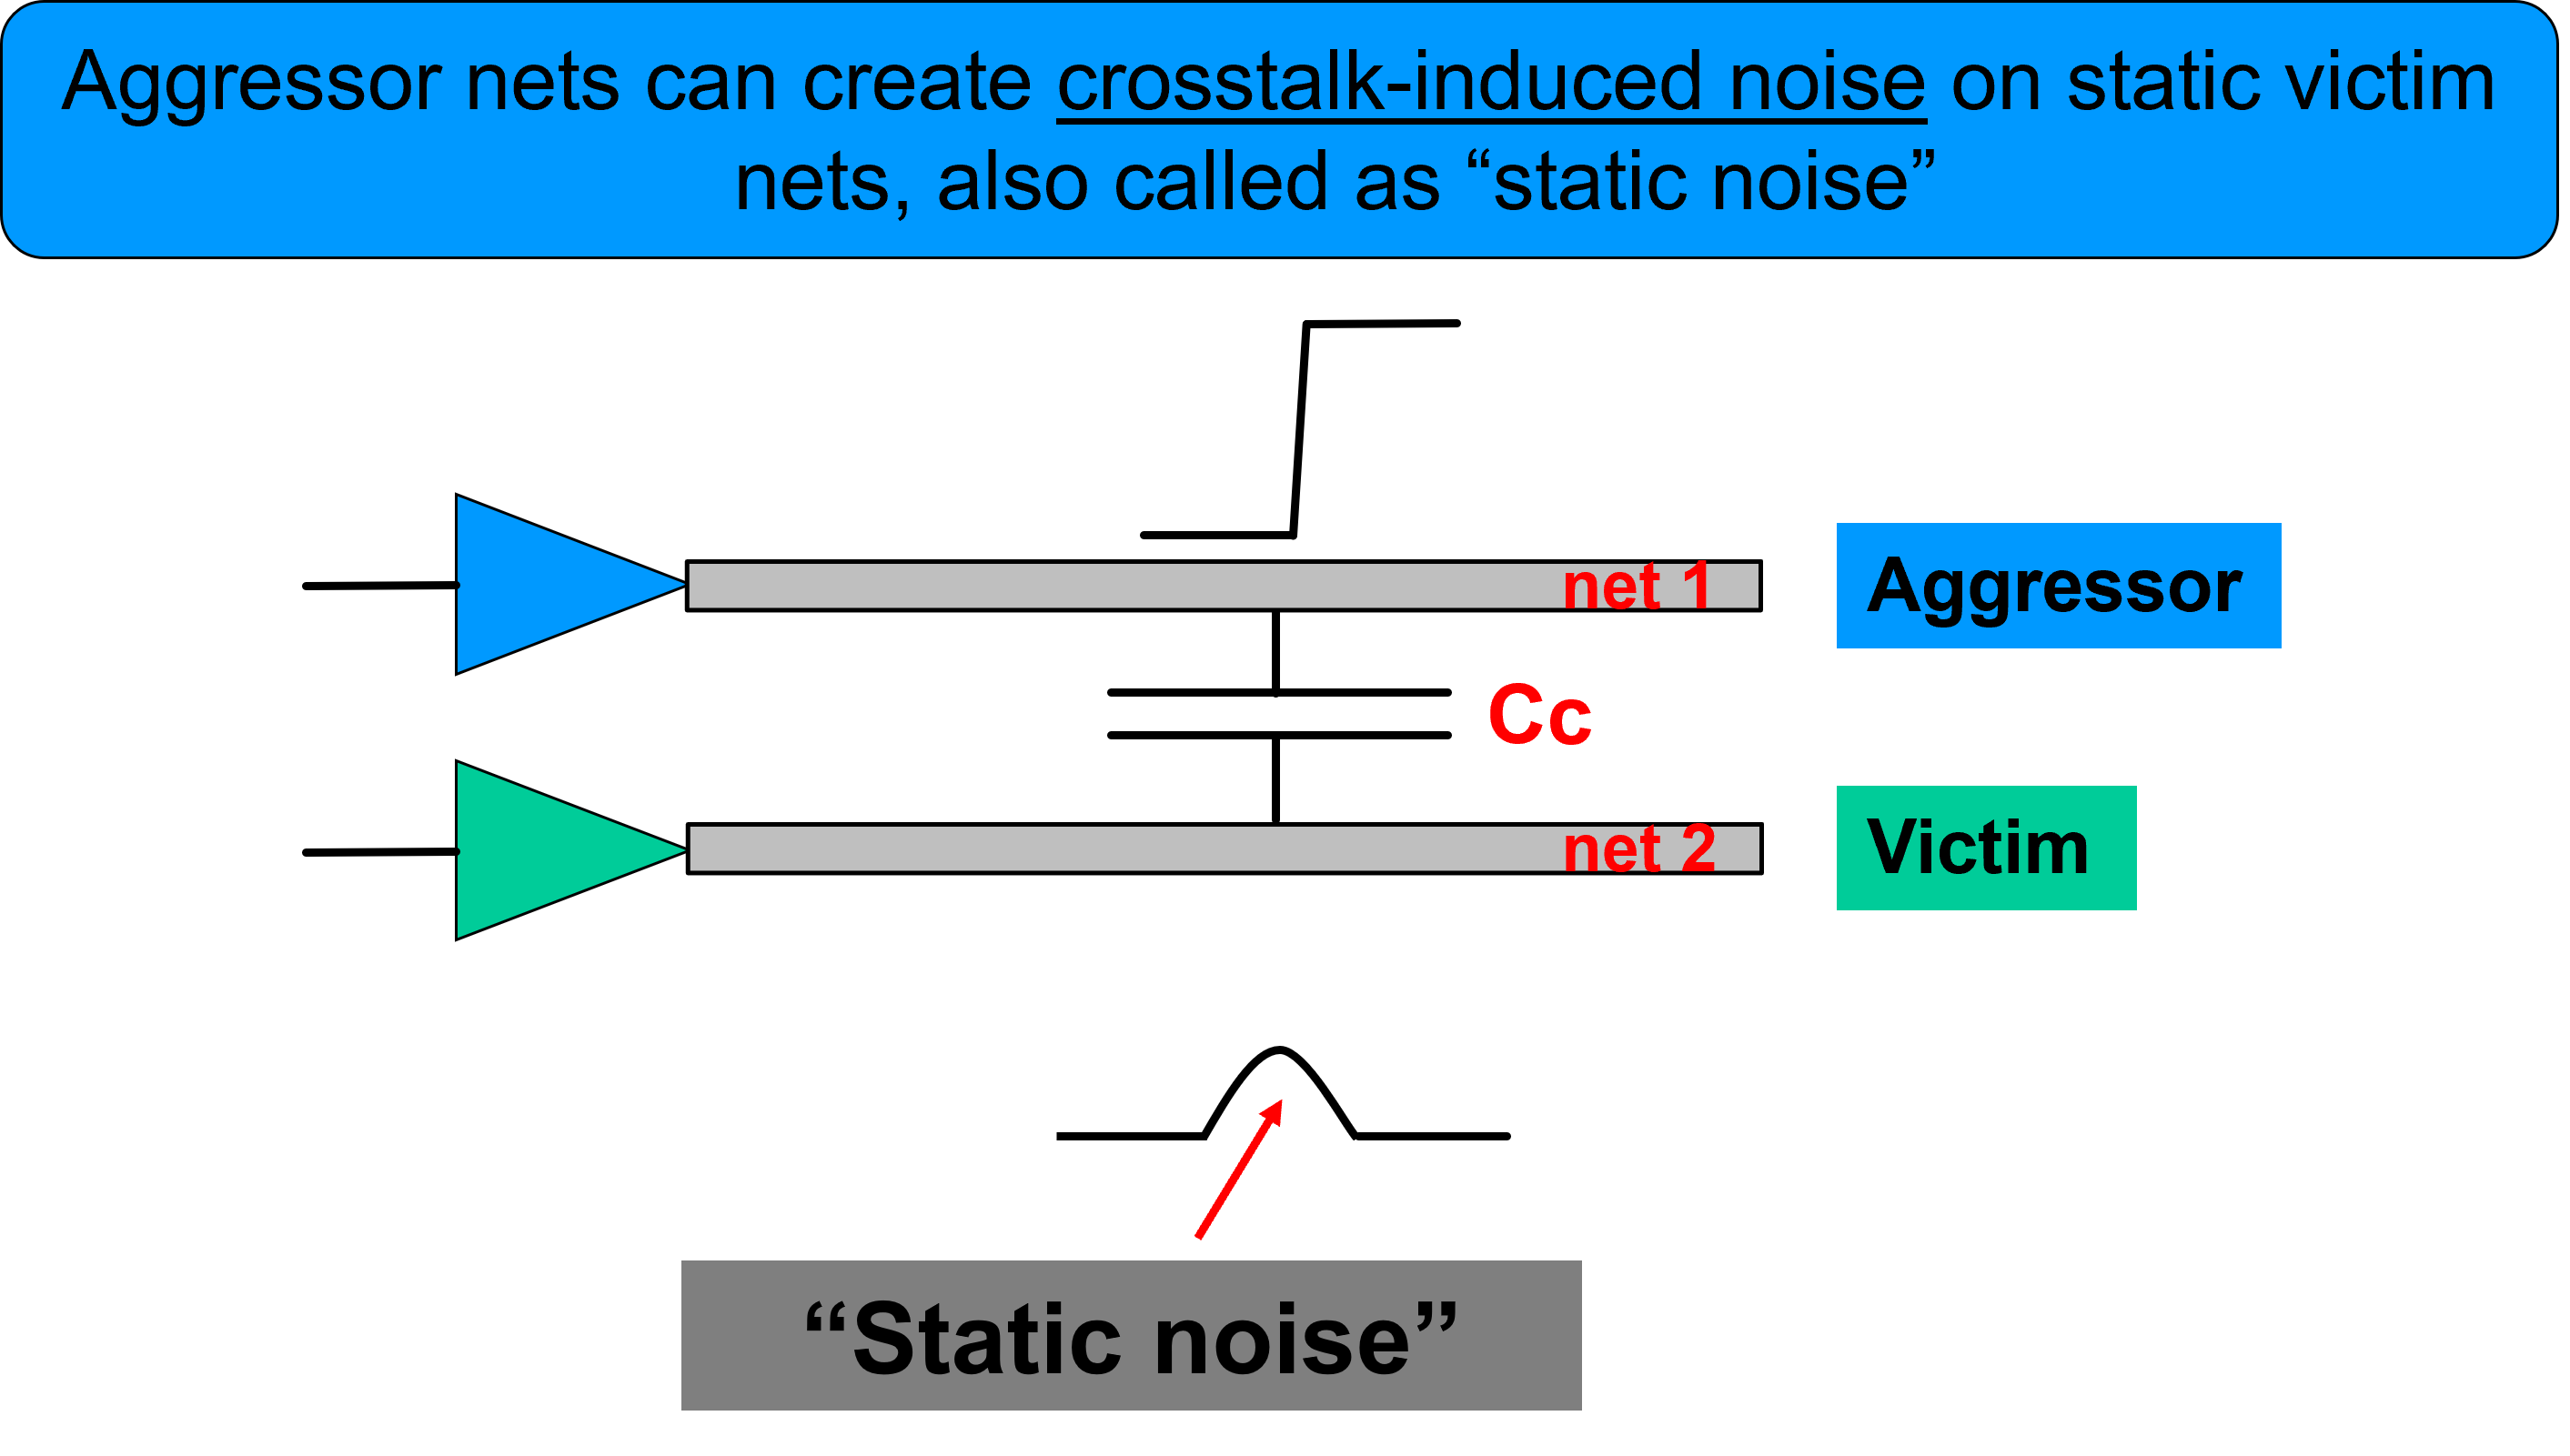
\includegraphics[width=\textwidth]{Glitches}
	\end{center}
\end{frame}


\begin{frame}
	\frametitle{Crosstalk-Induced Delay}
	\begin{center}
		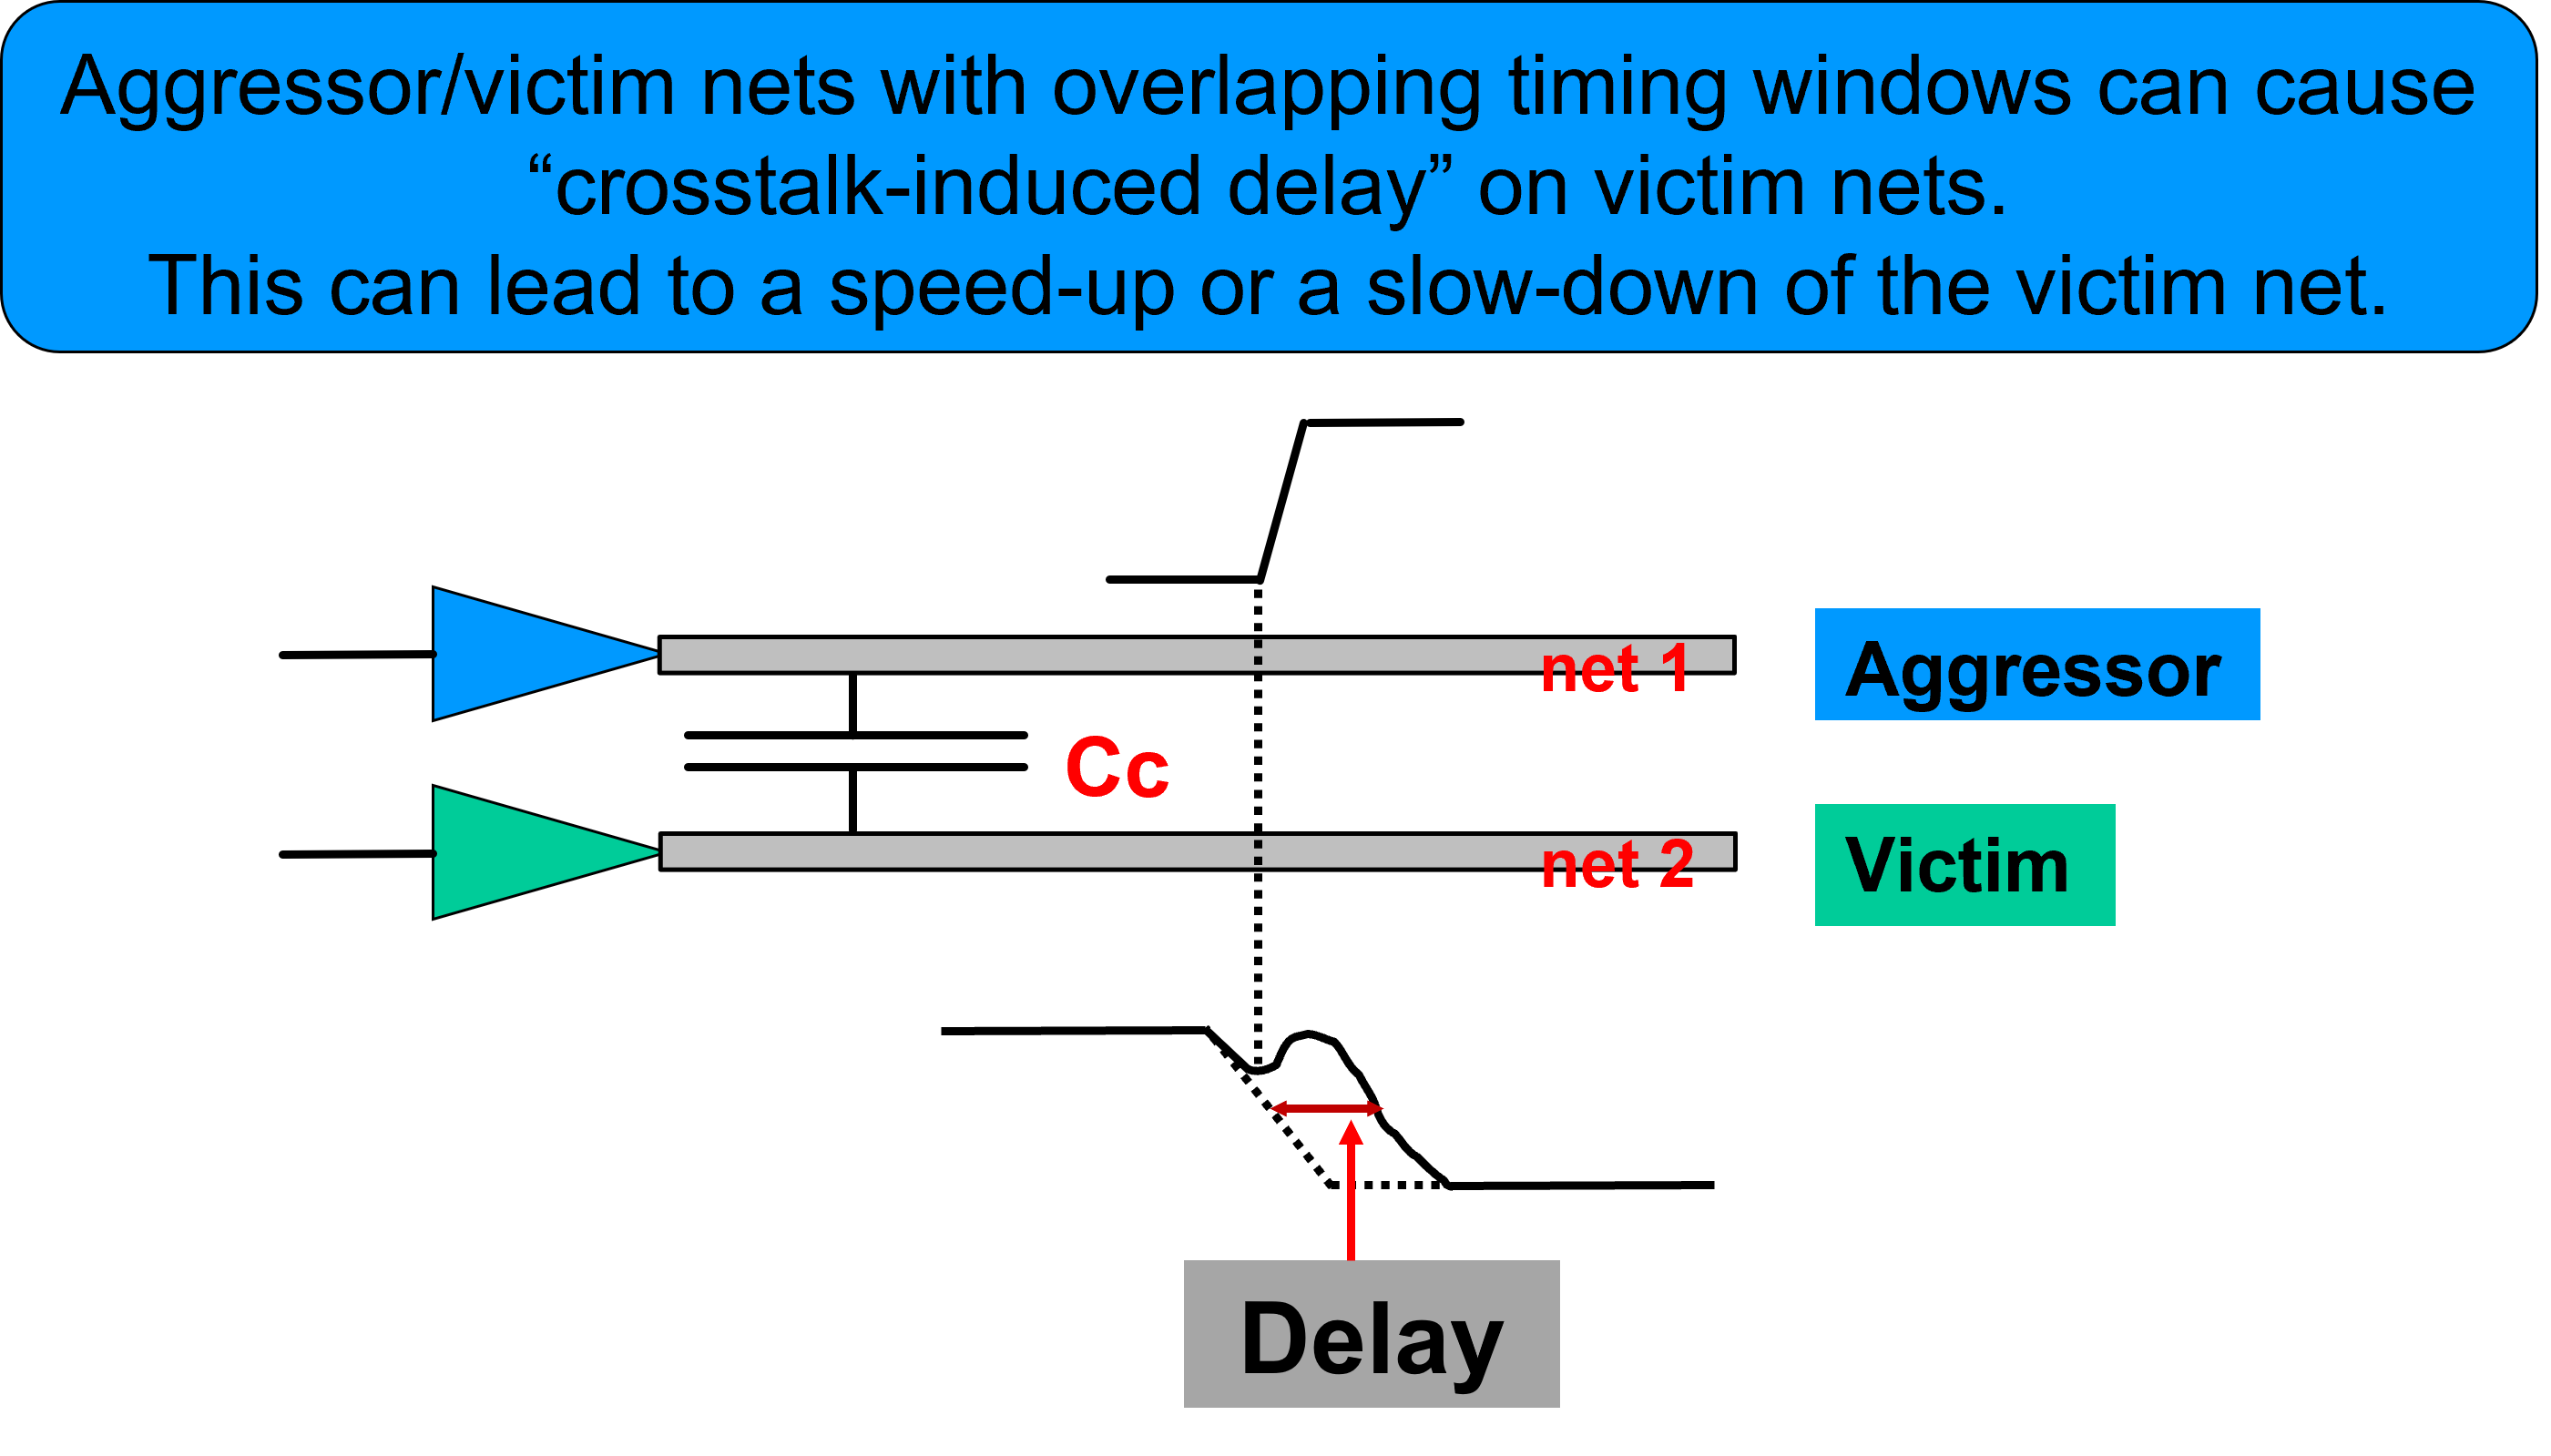
\includegraphics[width=\textwidth]{Delay}
	\end{center}
\end{frame}

\section[ECO]{Engineering change order (ECO) }
\subsection[ECO]{Engineering change order (ECO) }
\begin{frame}
	\frametitle{Engineering change order}
	\begin{center}
		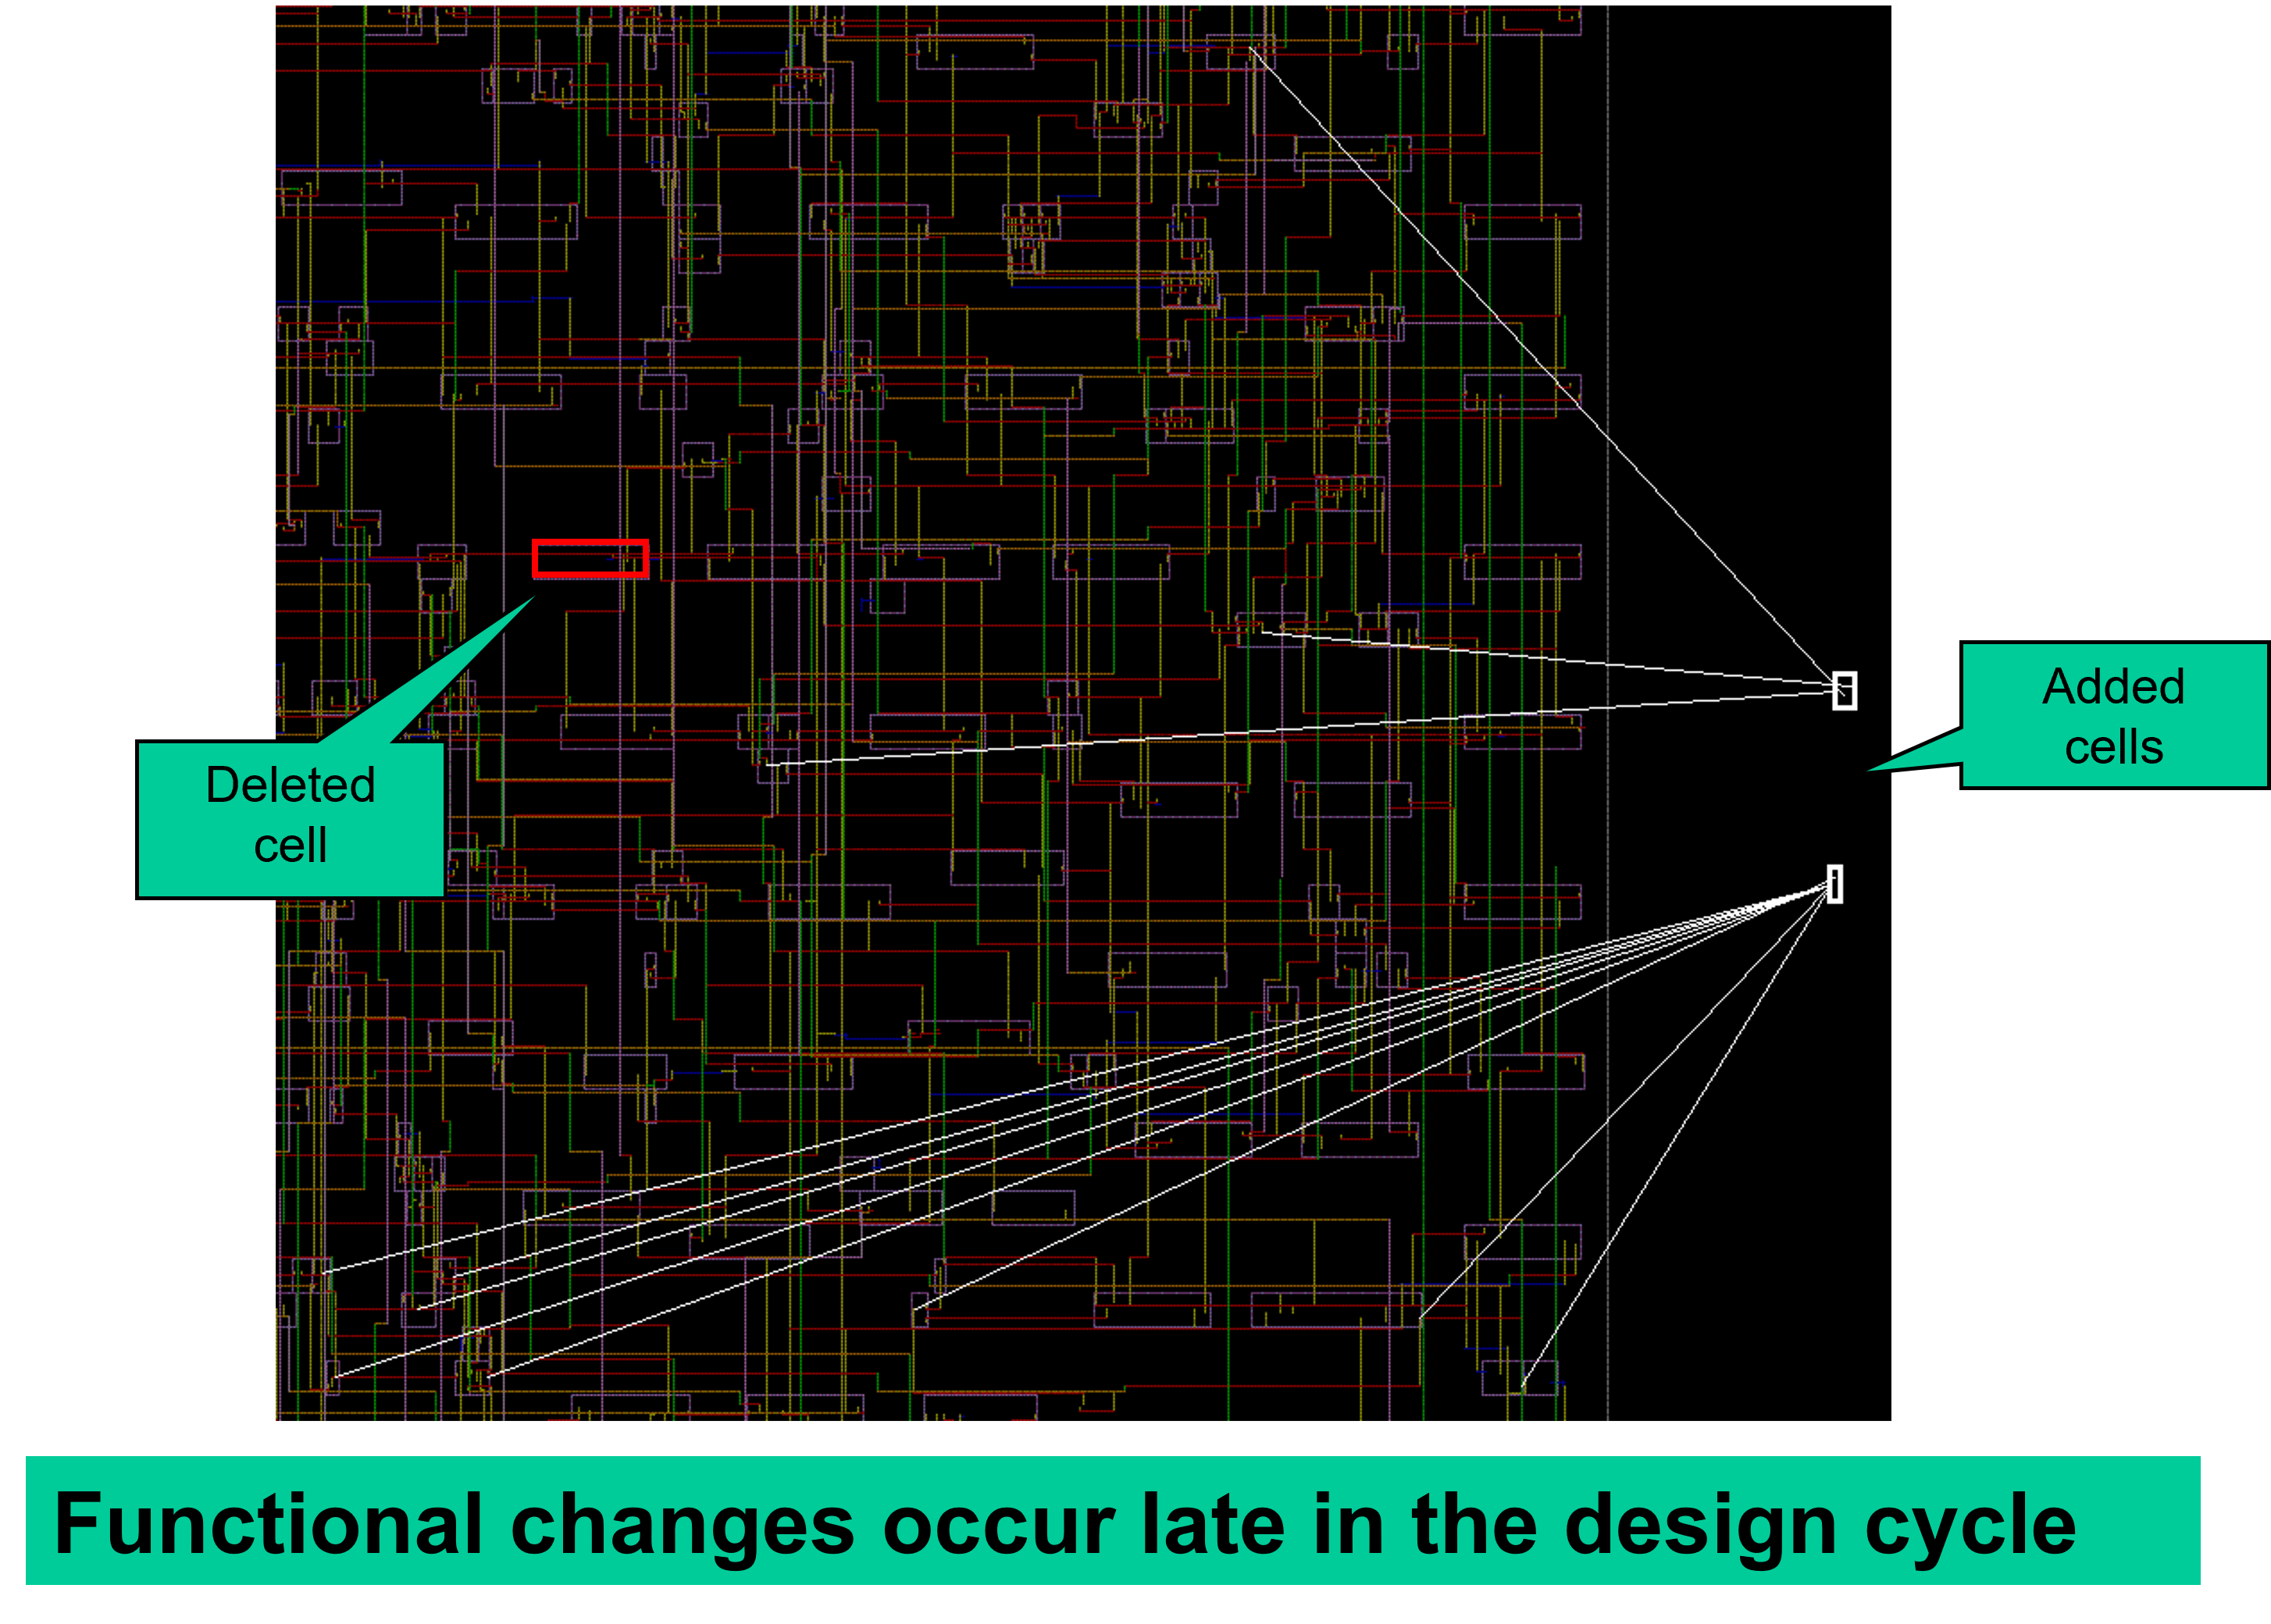
\includegraphics[width=\textwidth]{ECO}
	\end{center}
\end{frame}

\begin{frame}
	\frametitle{Two Types of ECO Flows}
	\begin{center}
		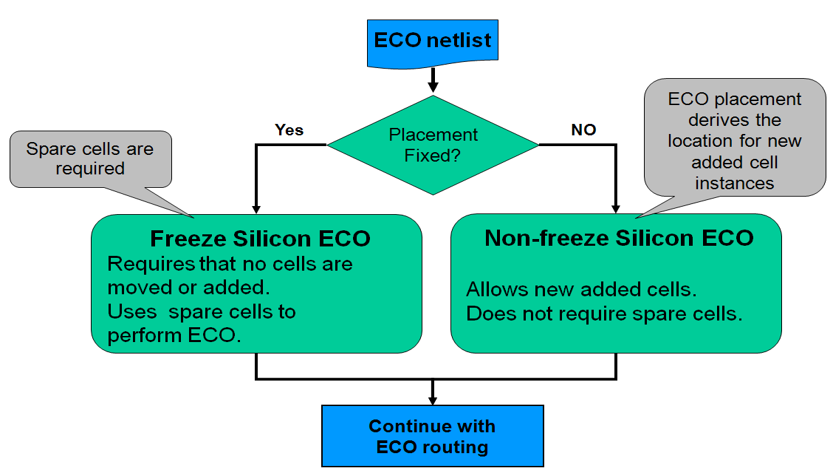
\includegraphics[width=\textwidth]{Types}
	\end{center}
\end{frame}
\subsection[Functional]{Functional ECO Flows}
\begin{frame}
	\frametitle{Functional ECO Flows}
	\begin{itemize}
		\item \textbf{Non-Freeze silicon ECO}
		\begin{itemize}
			\item Pre-tapeout, no restriction on placement or routing
			\item Minimal disturbances to the existing layout
			\item ECO cells are placed close to their optimal locations
		\end{itemize}
		\item \textbf{Freeze silicon ECO}
		\begin{itemize}
			\item Post-tapeout, metal masks change only using previously inserted spare cells
			
			\item Cell placement remains unchanged
			
			\item ECO cells are mapped to spare cells that are closest to the optimal location
			
			\item Deleted cells become spare cells
			
		\end{itemize}
	\end{itemize}
\end{frame}

\section[DFM]{Chip Finishing and DFM }
\subsection[Flow]{Chip Finishing Flow}
\begin{frame}
	\frametitle{Chip Finishing Flow}
	\begin{itemize}
		\item \textbf{PnR Compiler can address several issues to increase manufacturing yield:}
		\begin{itemize}
			\item Gate Oxide integrity $\rightarrow$ antenna fixing
			\item Via resistance and reliability $\rightarrow$ extra contacts
			\item Random Particle defect $\rightarrow$ Wire spreading
			\item Metal erosion $\rightarrow$ metal slotting
			\item Metal liftoff $\rightarrow$ metal slotting
			\item Metal Over-Etching $\rightarrow$ metal fill
		\end{itemize}
	\end{itemize}
\end{frame}

\begin{frame}
	\frametitle{Manufacturability Issues}
	\begin{itemize}
		\item In deep submicron VLSI, some manufacturing steps, like photo-resist exposure, development and
		etch and Chemical Mechanical Polishing (CMP) have detrimental effects on interconnect
		structures. These effects can vary based on local characteristics of the layout.
		\item To make these effects predictable, the layouts must be made “uniform” with respect to certain
		density standards across very small localized areas of the die. In the past, foundries performed the
		post processing needed to provide this uniformity. The techniques they used were filling (selective
		insertion of shapes) or slotting (selective reduction of shapes).
		\item In today’s processes, the design tools doing RC extraction, delay calculation, IR drop analysis,
		timing/noise/crosstalk analysis must be aware of these slotting/filling activities or suffer
		significant inaccuracy.
		
	\end{itemize}
\end{frame}

\begin{frame}
	\frametitle{Manufacturability Issues}
	\begin{itemize}
		\item PnR Compiler attempts to move all these into the design stage and out of the Fab post processing regime.
		
		\item To minimize the impact of the manufacturing process on device yields, foundries impose various
		density rules to make the layouts more uniform. For instance, the foundry may impose a density
		rule on an interconnect layer such that in any 10 um x 10 um window, there must be at least 35
		um2 of metal features, but no greater than 70 um2 of metal.
		\item Spare areas must be filled, but wide metal stripes must be slotted to meet the density rules.
	\end{itemize}
\end{frame}

\subsection[Antenna]{Antenna Fixing}
\begin{frame}
	\frametitle{Problem: Gate Oxide Integrity}
	\begin{itemize}
		\item \textbf{Metal wires (antennae) placed in an EM field
		generate voltage gradients}
		\item \textbf{During the metal etch stage, strong EM fields are
		used to stimulate the plasma etchant}
		\item \textbf{Resultant voltage gradients at MOSFET gates can
		damage the thin oxide}
	\end{itemize}
	\begin{center}
		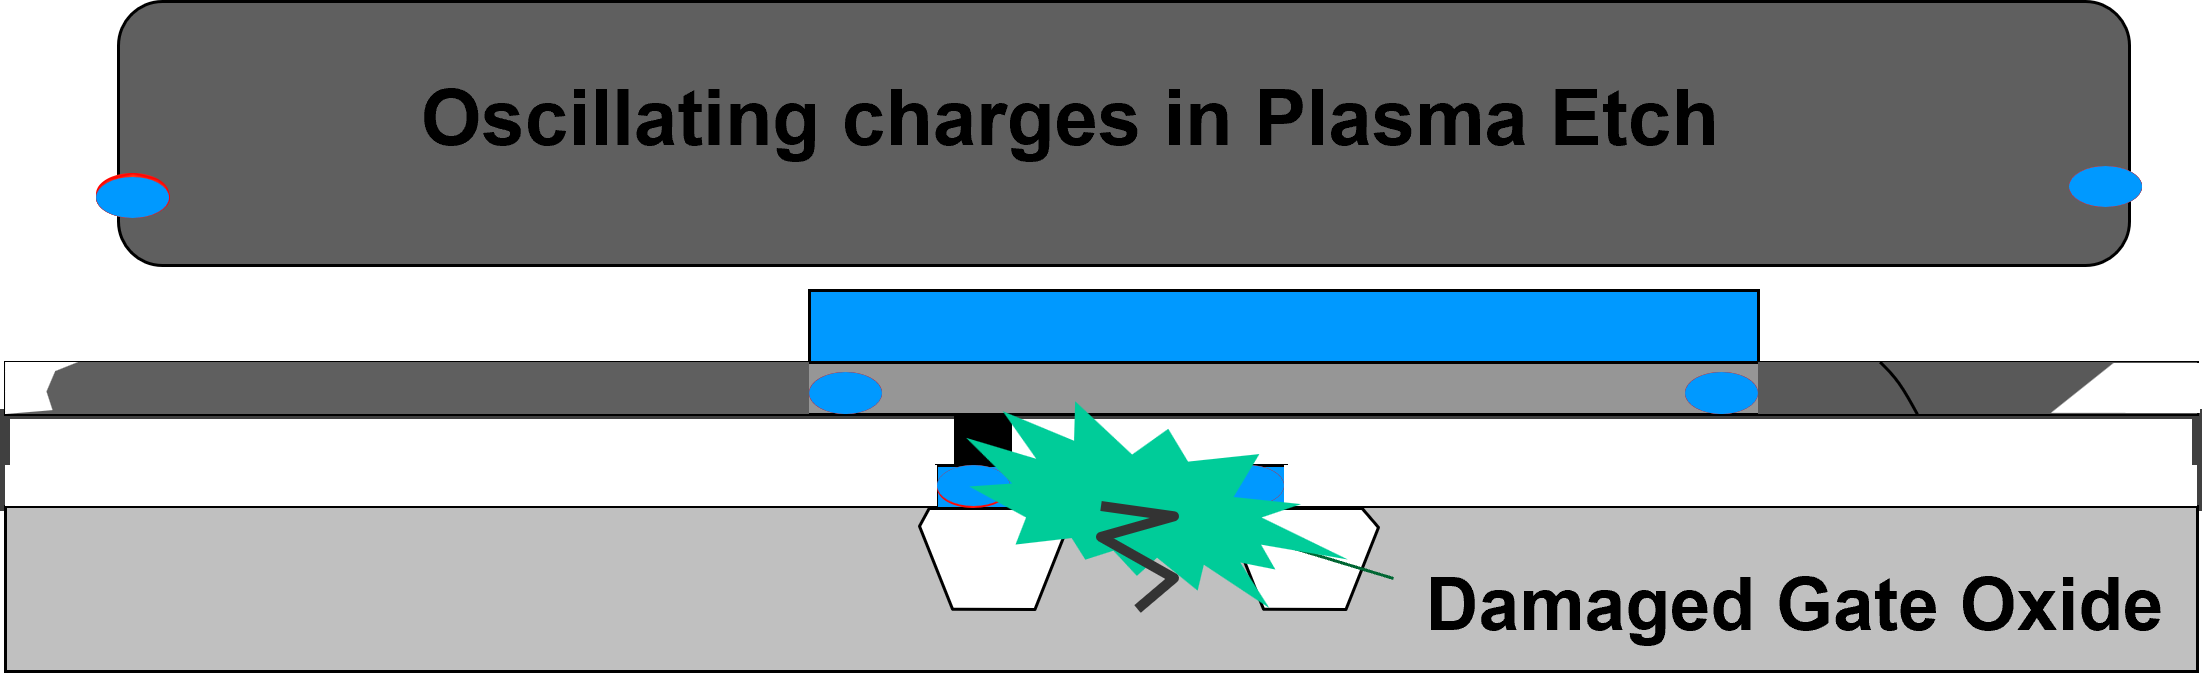
\includegraphics[width=0.7\textwidth]{Antenna}
	\end{center}
\end{frame}

\begin{frame}
	\frametitle{Antenna Rules}
	\begin{itemize}
		\item \textbf{As length of wire increases during processing, the
		voltage stressing the gate oxide increases}
		\item \textbf{Antenna rules define acceptable length of wires}
	\end{itemize}
\begin{center}
	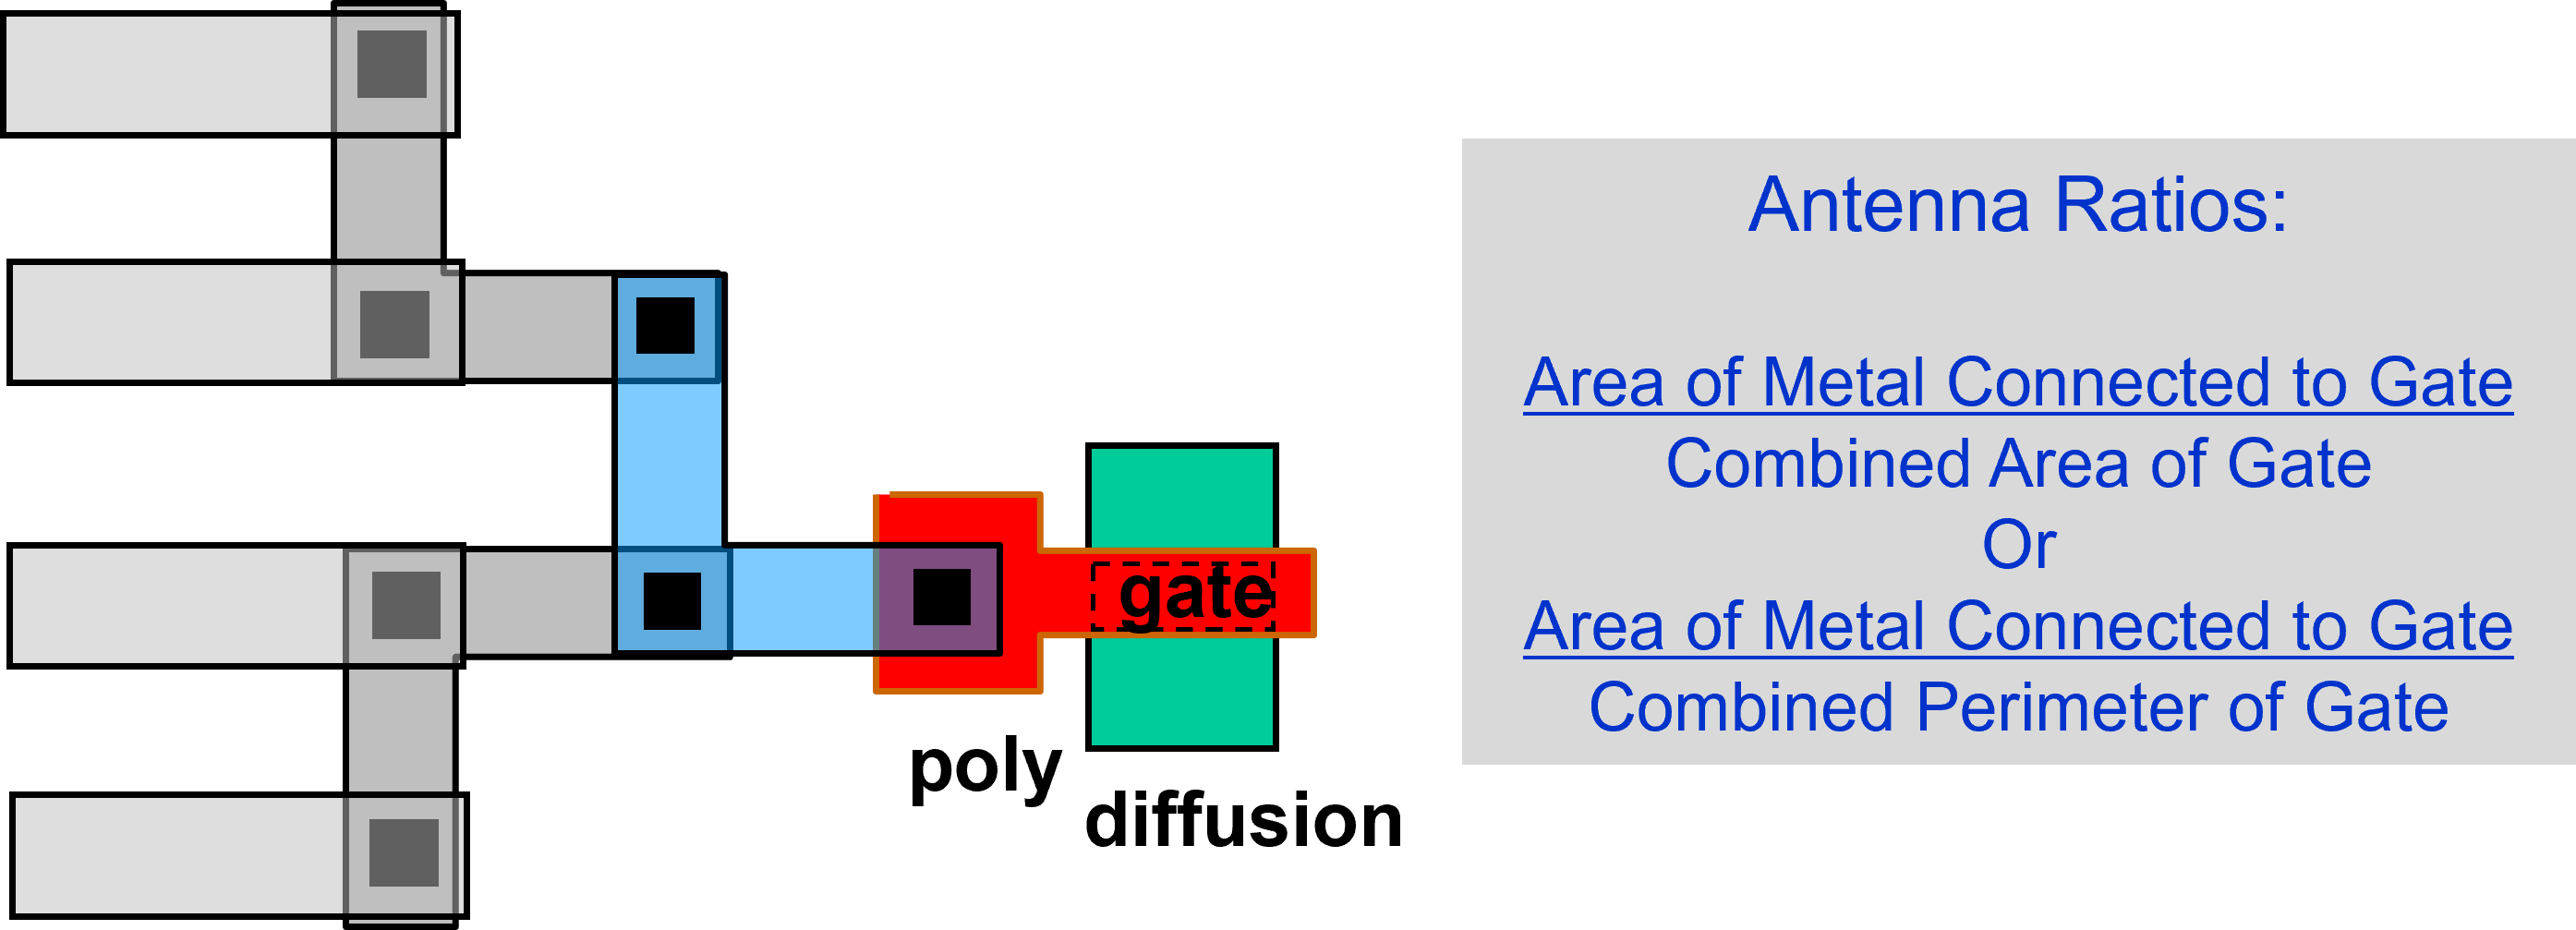
\includegraphics[width=0.8\textwidth]{Rules}
\end{center}
\end{frame}

\begin{frame}
	\frametitle{Fixing Antenna Problems}
	\begin{center}
		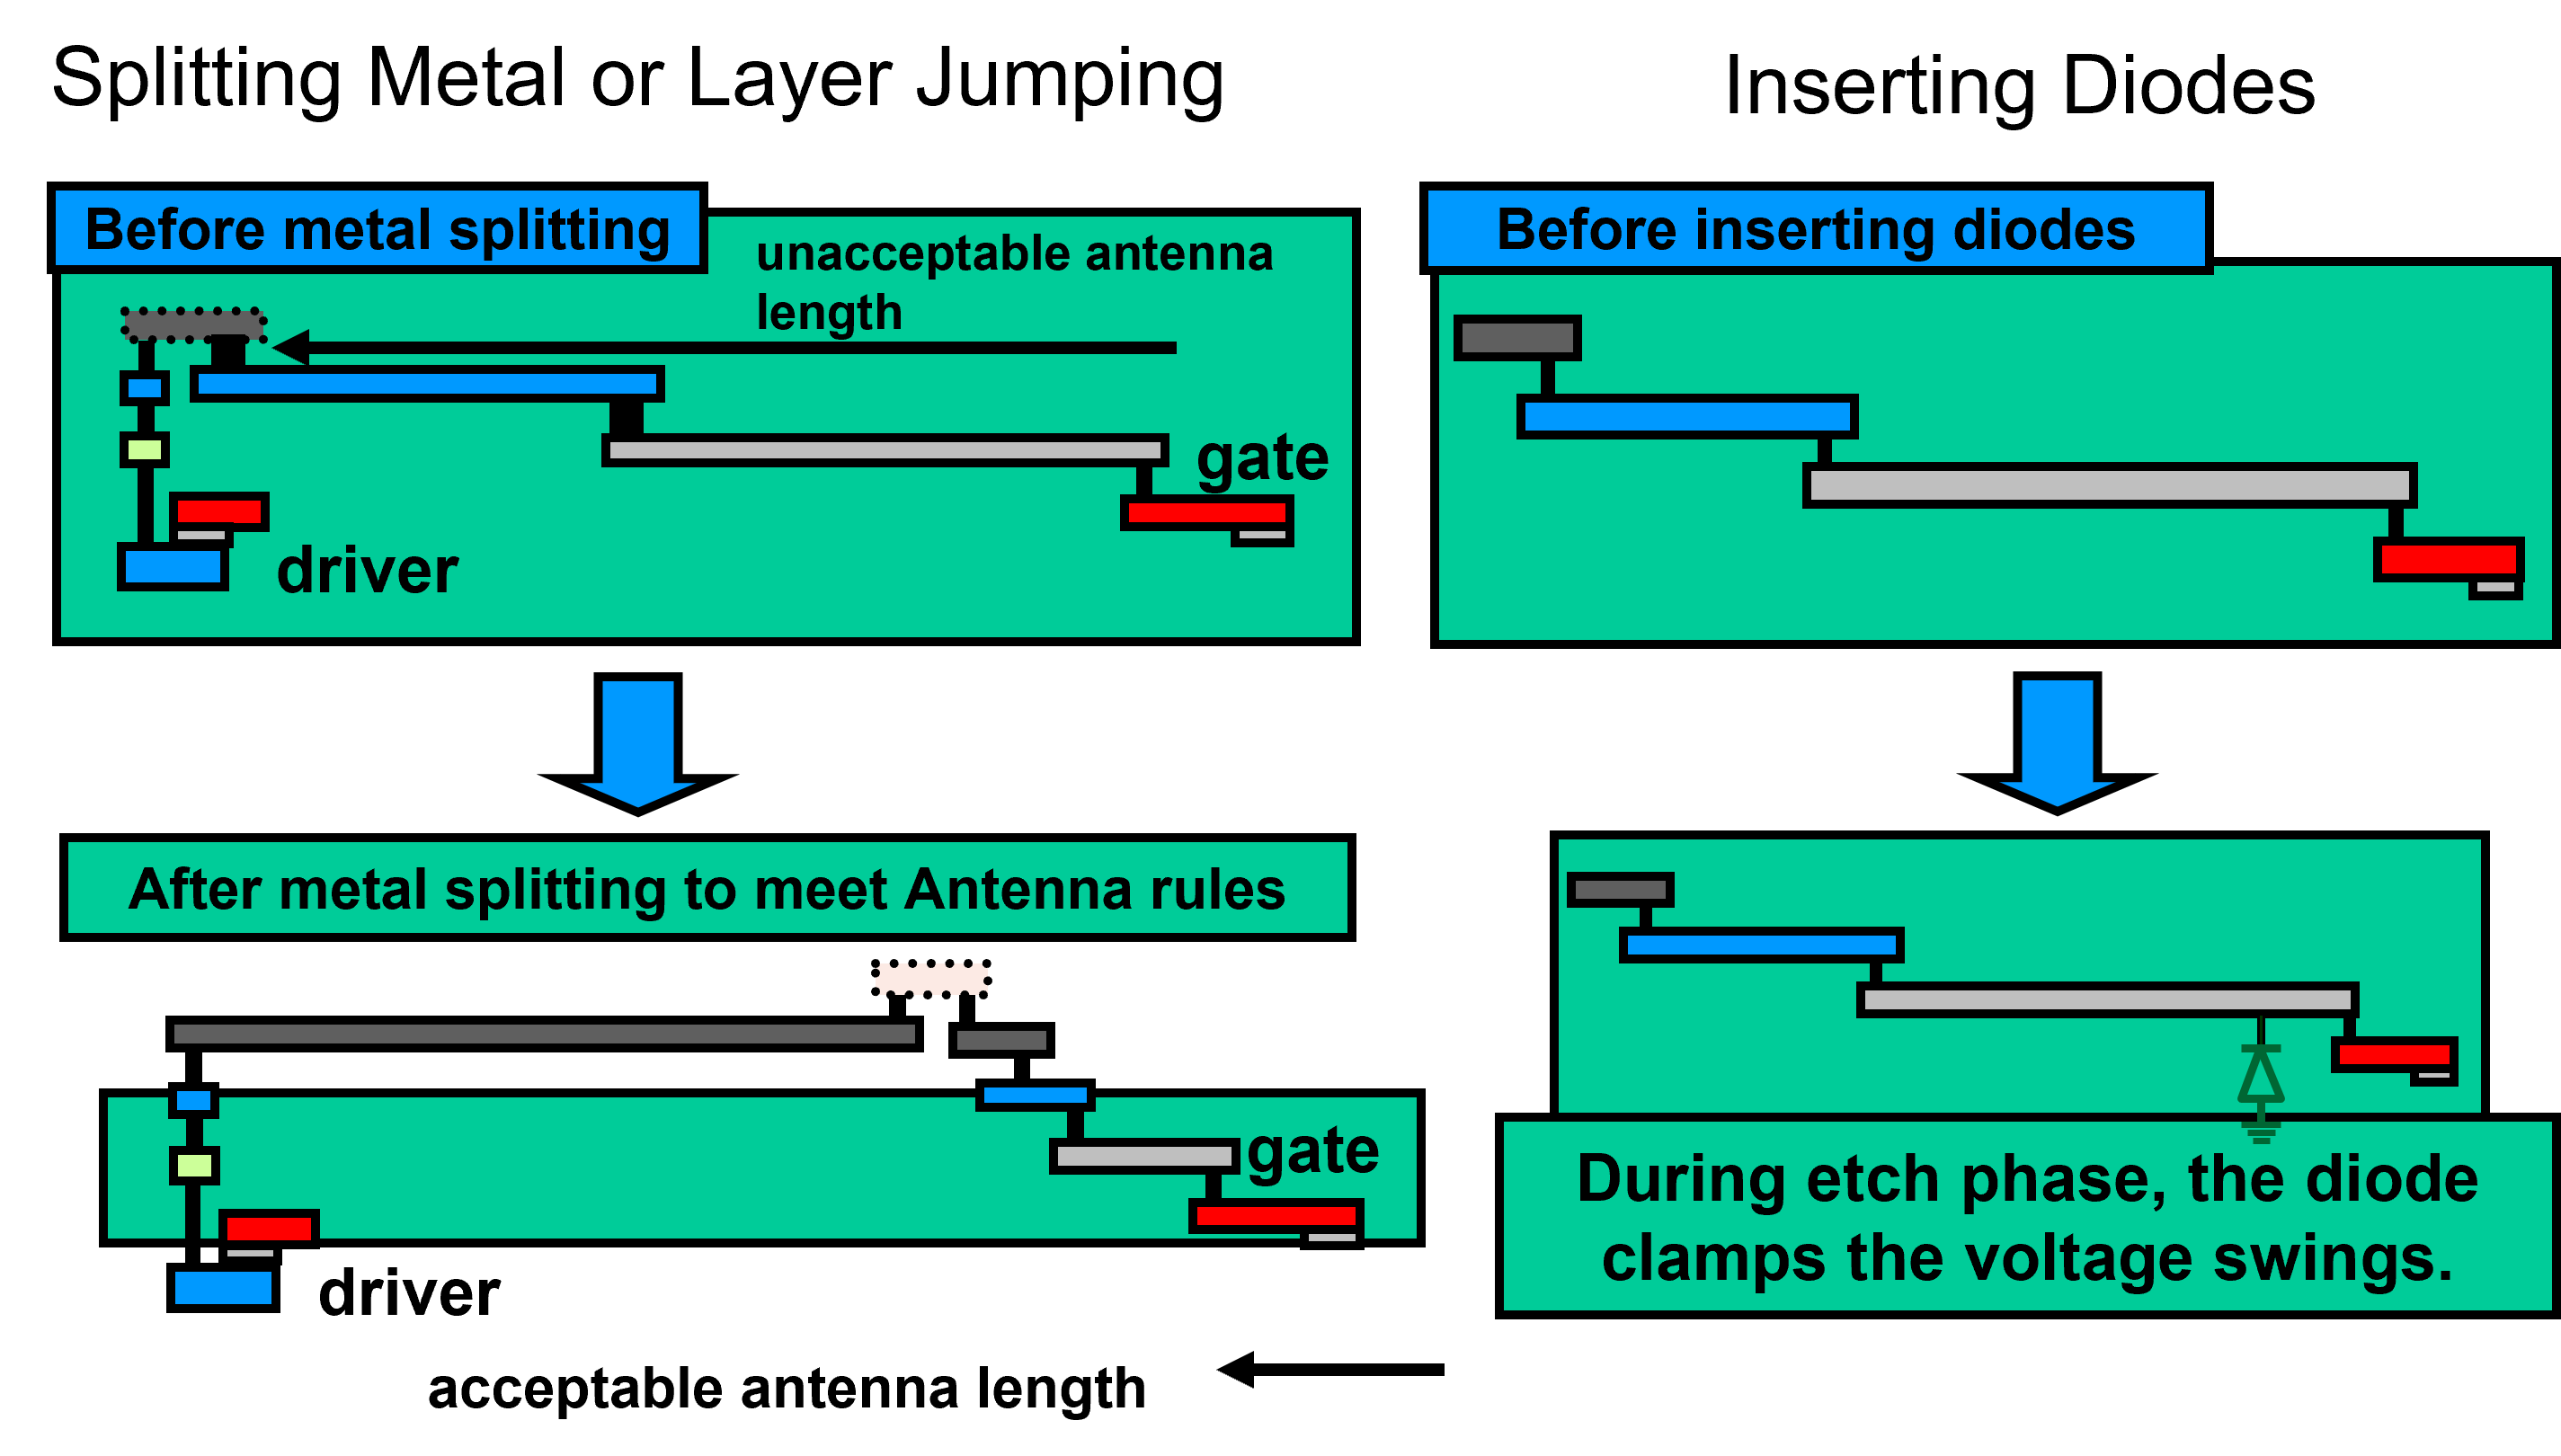
\includegraphics[width=\textwidth]{Fixing}
	\end{center}
\end{frame}

\subsection[Via]{Redundant Via Insertion}
\begin{frame}
	\frametitle{Voids in Vias During Manufacturing}
	\begin{itemize}
		\item \textbf{Voids in vias is a serious issue in manufacturing}
		\item \textbf{Two solutions are available:}
		\begin{itemize}
			\item Reduce via count: via optimization techniques are employed in routing stage
			\item Add backup vias: known as \underline{redundant vias}
		\end{itemize}
	\end{itemize}
\begin{center}
	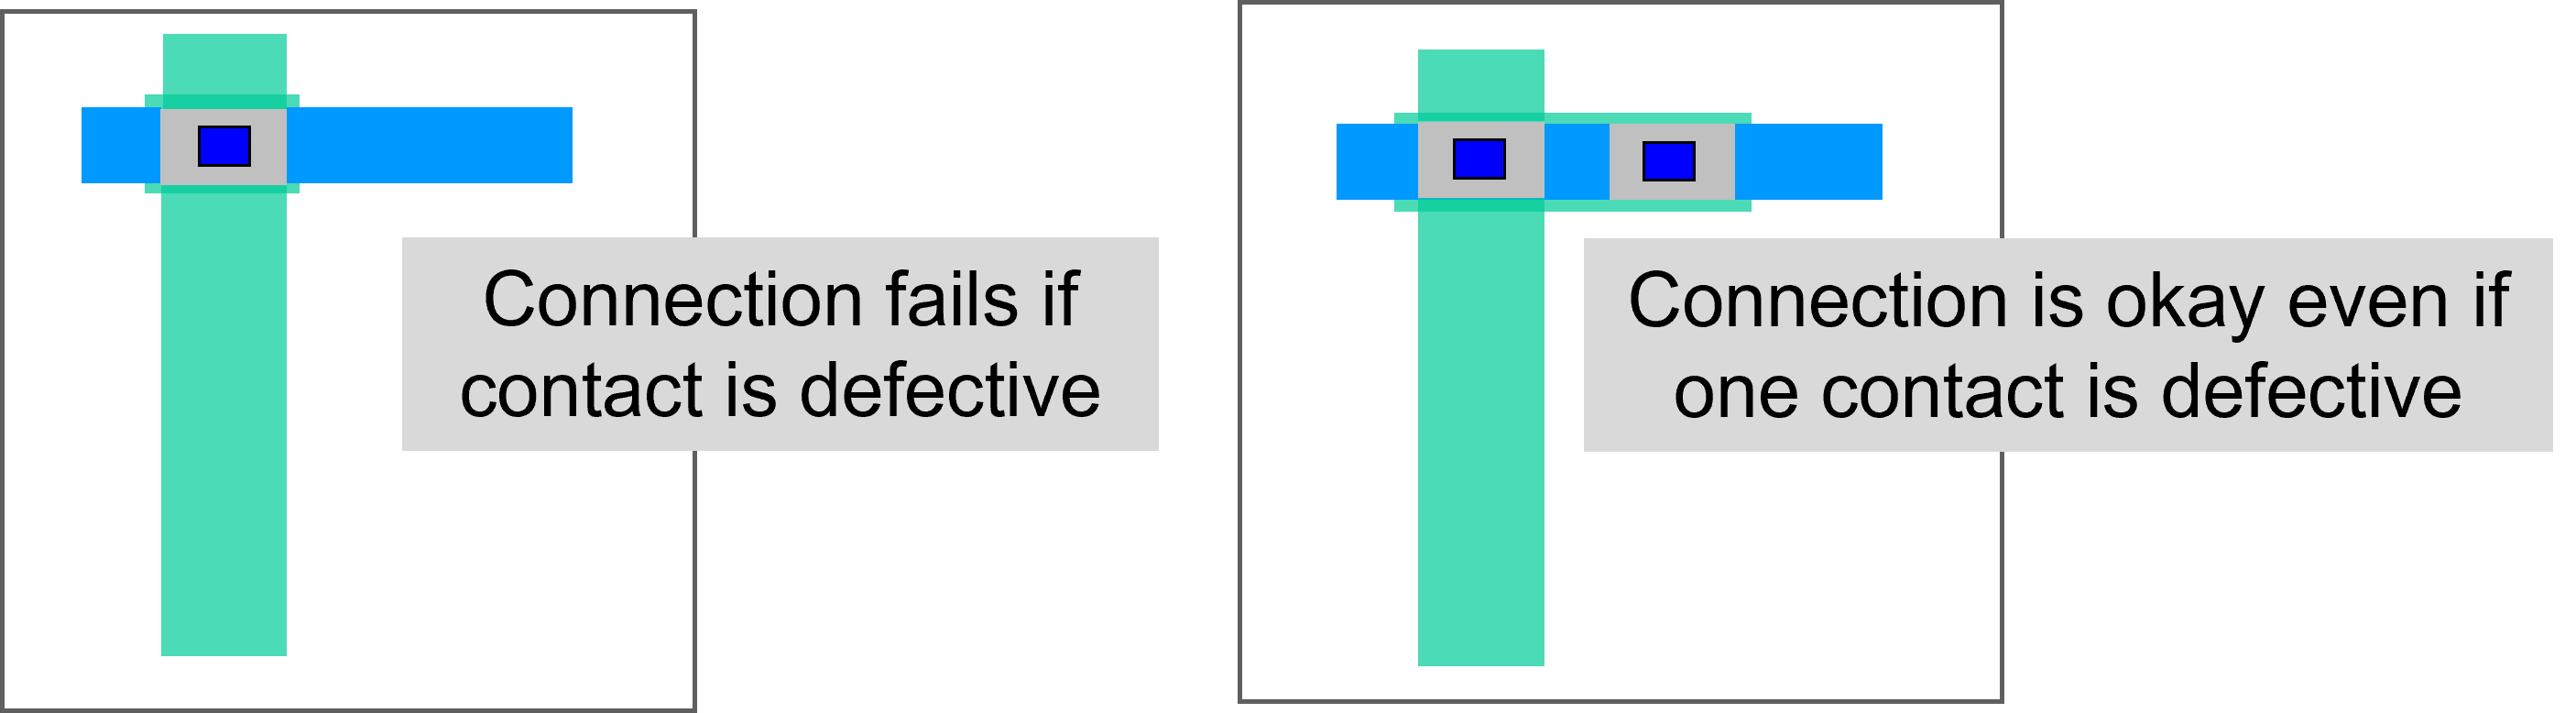
\includegraphics[width=\textwidth]{vias}
\end{center}
\end{frame}
\begin{frame}
	\frametitle{Via Resistance and Reliability}
	\begin{itemize}
		\item \textbf{Replacing one via with multiple vias can improve
		yield \& timing (series R reduction)}
		\item \textbf{Inserts multiple vias without rerouting}
	\end{itemize}
\begin{center}
	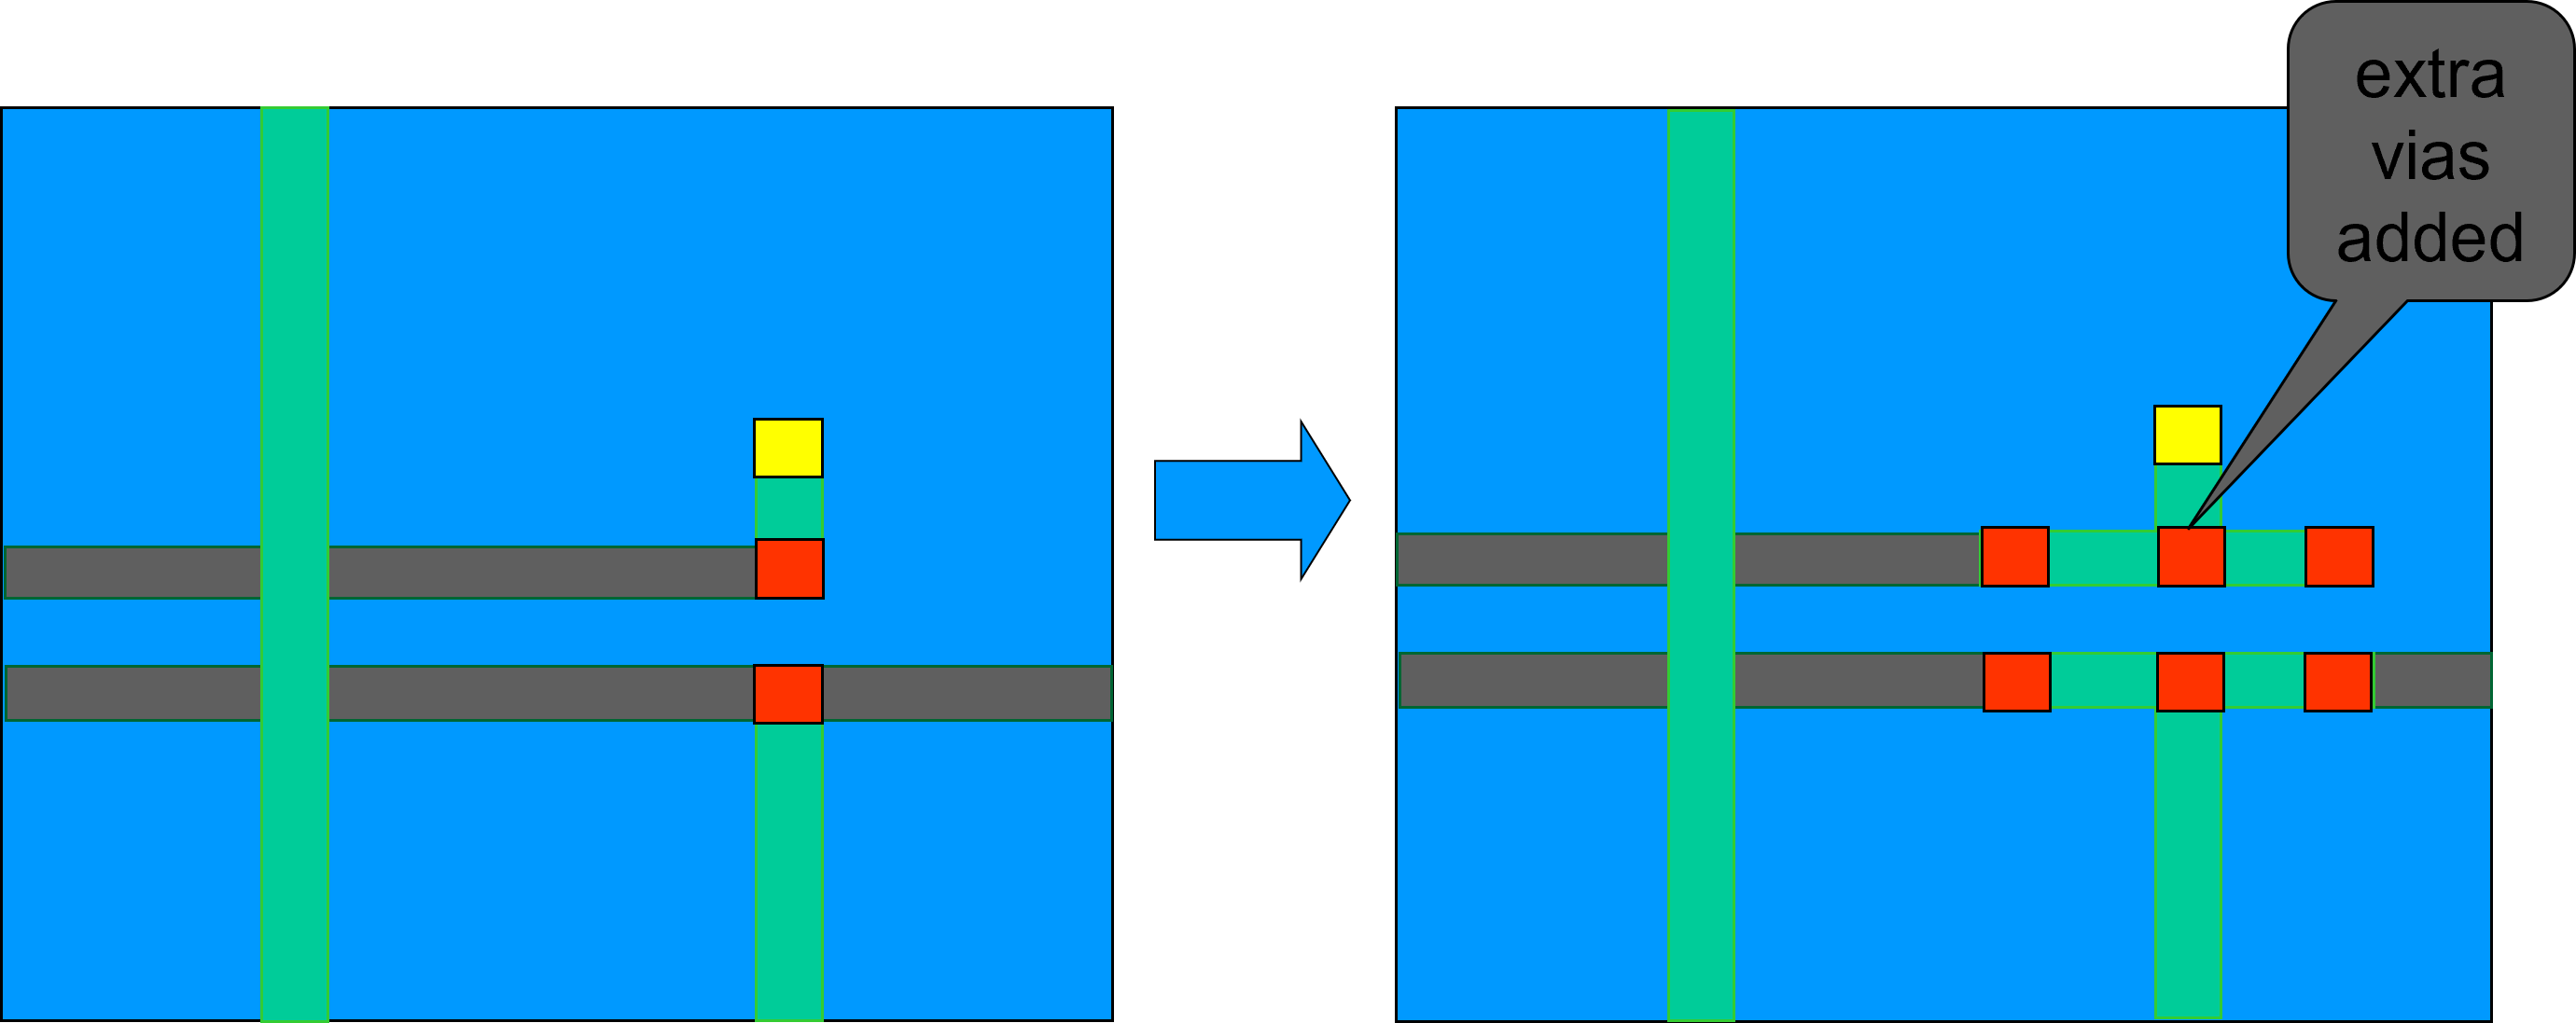
\includegraphics[width=\textwidth]{Via}
\end{center}
\end{frame}

\subsection[Wire]{Wire Spreading}
\begin{frame}
	\frametitle{Wire Spreading: Random Particle Defects }
	\begin{itemize}
		\item \textbf{Random missing or extra material causes opens or
			shorts during the fabrication process}
		\begin{itemize}
			\item Wires at minimum spacing are most susceptible to shorts
			\item Minimum-width wires are most susceptible to opens
		\end{itemize}
	\end{itemize}
\begin{center}
	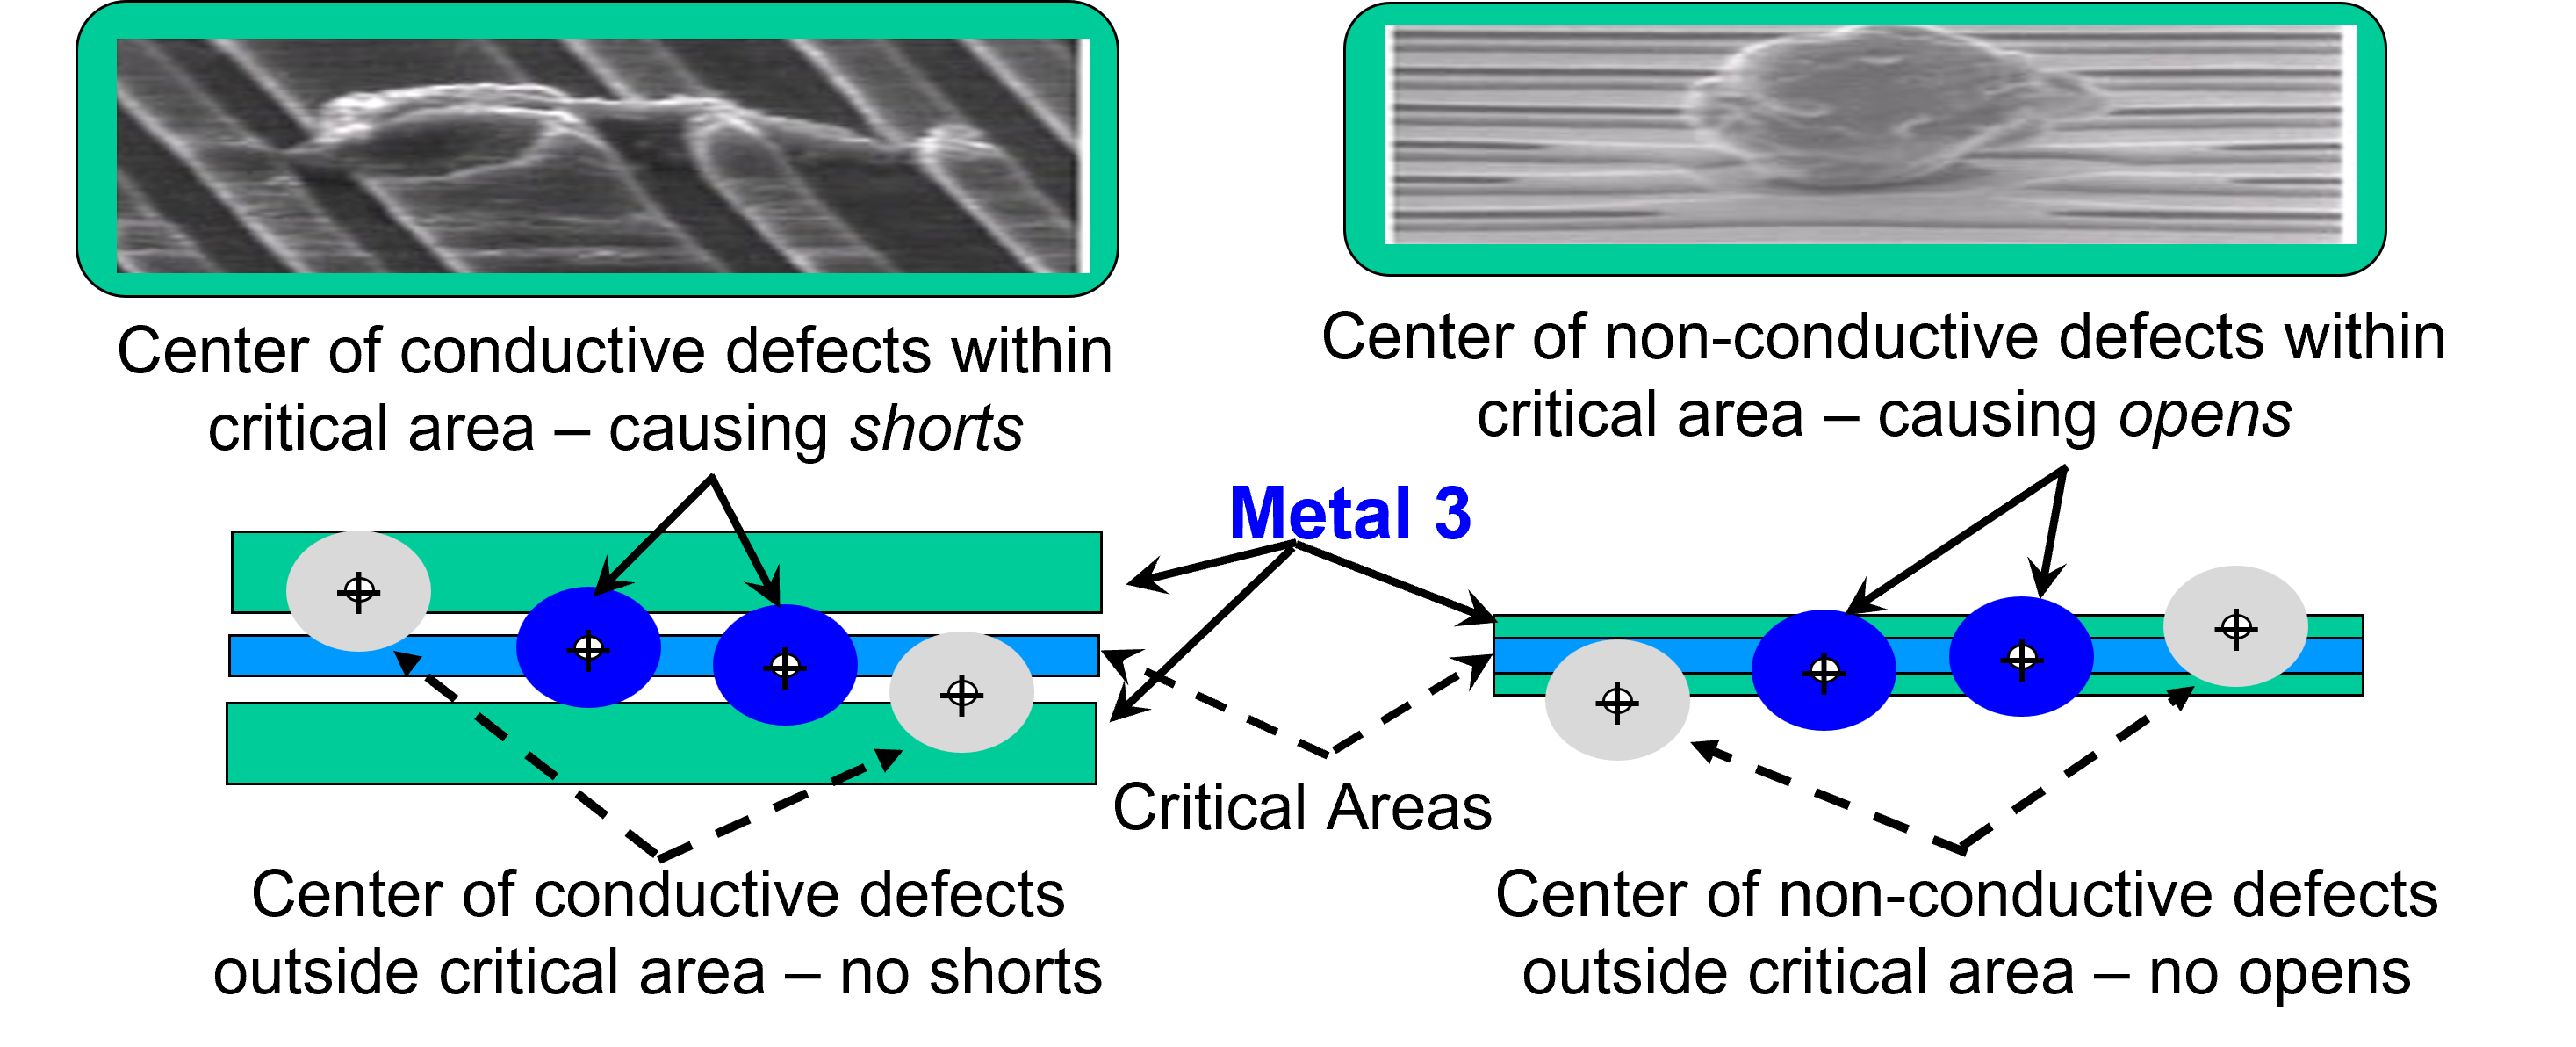
\includegraphics[width=0.7\textwidth]{wire}
\end{center}
\end{frame}

\subsection[Filler]{Filler Cell Insertion}
\begin{frame}
	\frametitle{Filler Cell Insertion}
	\begin{itemize}
		\item \textbf{Metal fill insertion helps }
		\begin{itemize}
			\item To fill layers of choice including poly
			\item To insert floating vias 
			\item To do area based metal fill 
			\item To specify required width (timing driven metal fill doesn’t fill wire tracks around critical nets)
			
		\end{itemize}
		\item \textbf{For better yield, density of the chip needs to be uniform}
		\item \textbf{Some placement sites remain empty on some rows}
		
	\end{itemize}
\end{frame}

\subsection[Metal]{Metal Fill Insertion}
\begin{frame}
	\frametitle{Problem: Metal Over-Etching}
	\begin{itemize}
		\item \textbf{A narrow metal wire separated from other metal receives a higher density of etchant than closely spaced wires}
		\item \textbf{The narrow metal can get over-etched}
		\item \textbf{\underline{Minimum} metal density rules are used to control this}
	\end{itemize}
\begin{center}
	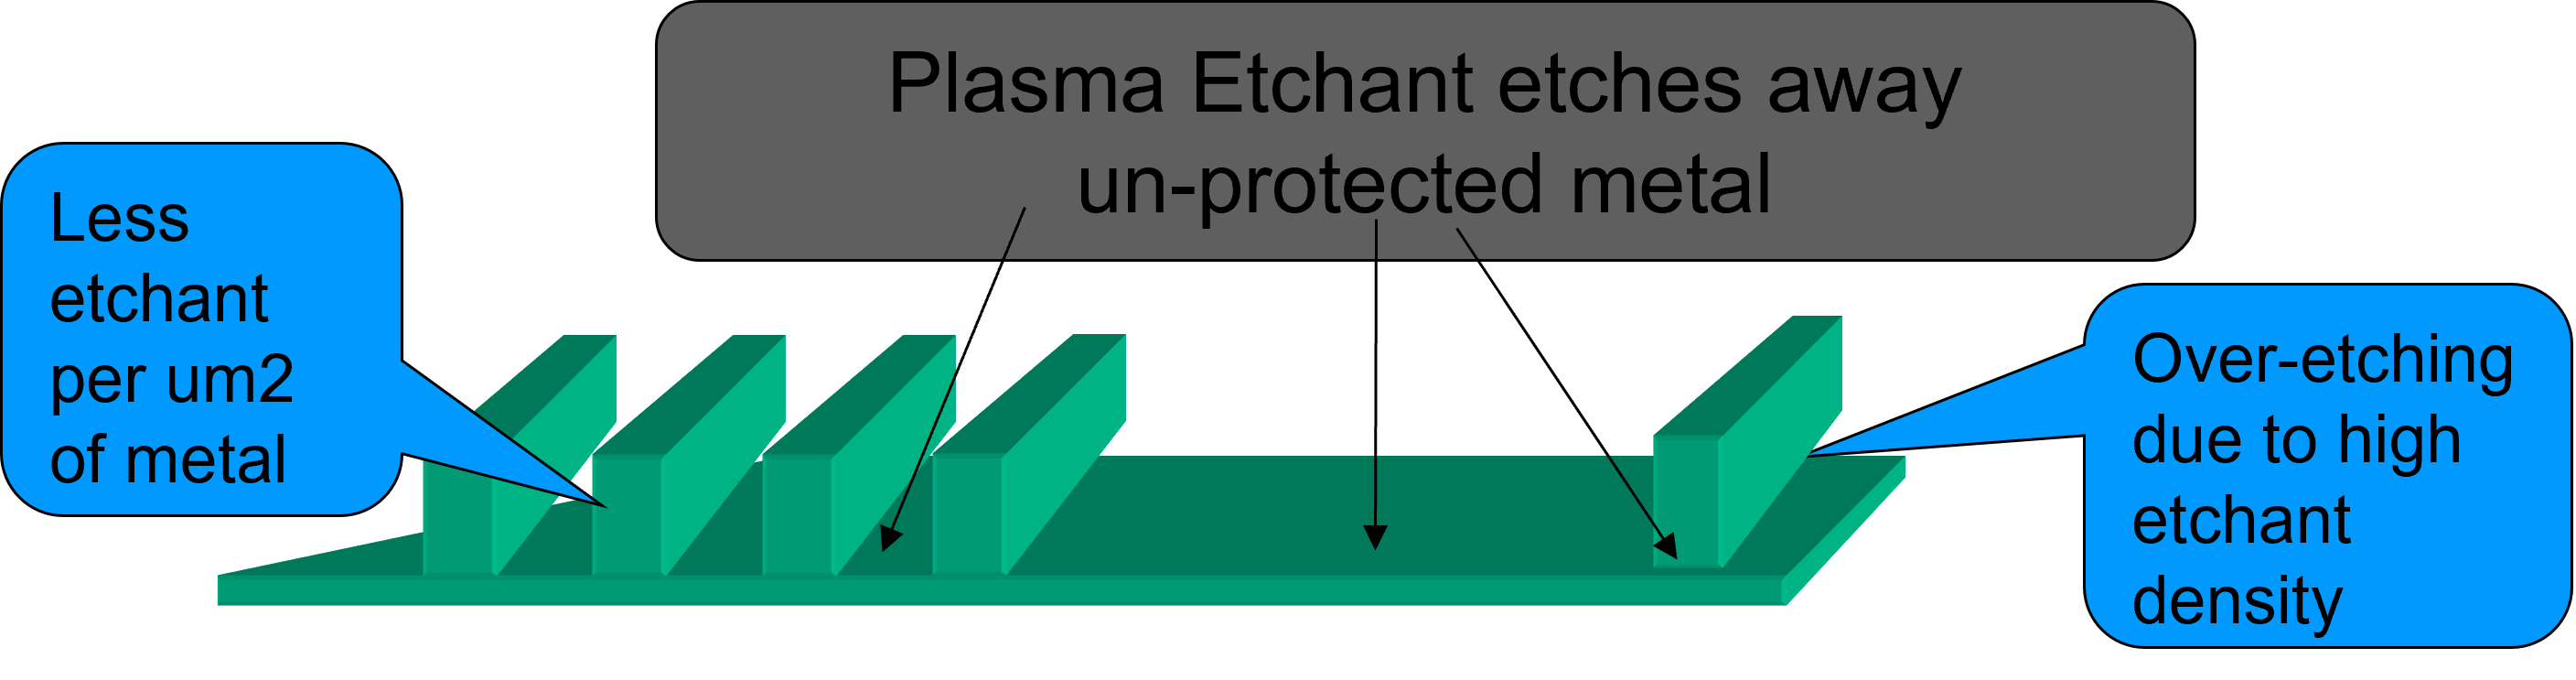
\includegraphics[width=0.7\textwidth]{Metal}
\end{center}
\begin{itemize}
	\item Too much etchant in contact with too little metal $\rightarrow$ over-etched metal
	
\end{itemize}
\end{frame}

\begin{frame}
	\frametitle{Solution: Metal Fill}
	\begin{itemize}
		\item \textbf{Fills empty tracks with metal shapes to meet the
		minimum metal density rules}
		\item \textbf{Uses up most of the remaining routing resource:}
		\begin{itemize}
			\item No further routing or antenna fixes can be done
		\end{itemize}
	\end{itemize}
\begin{center}
	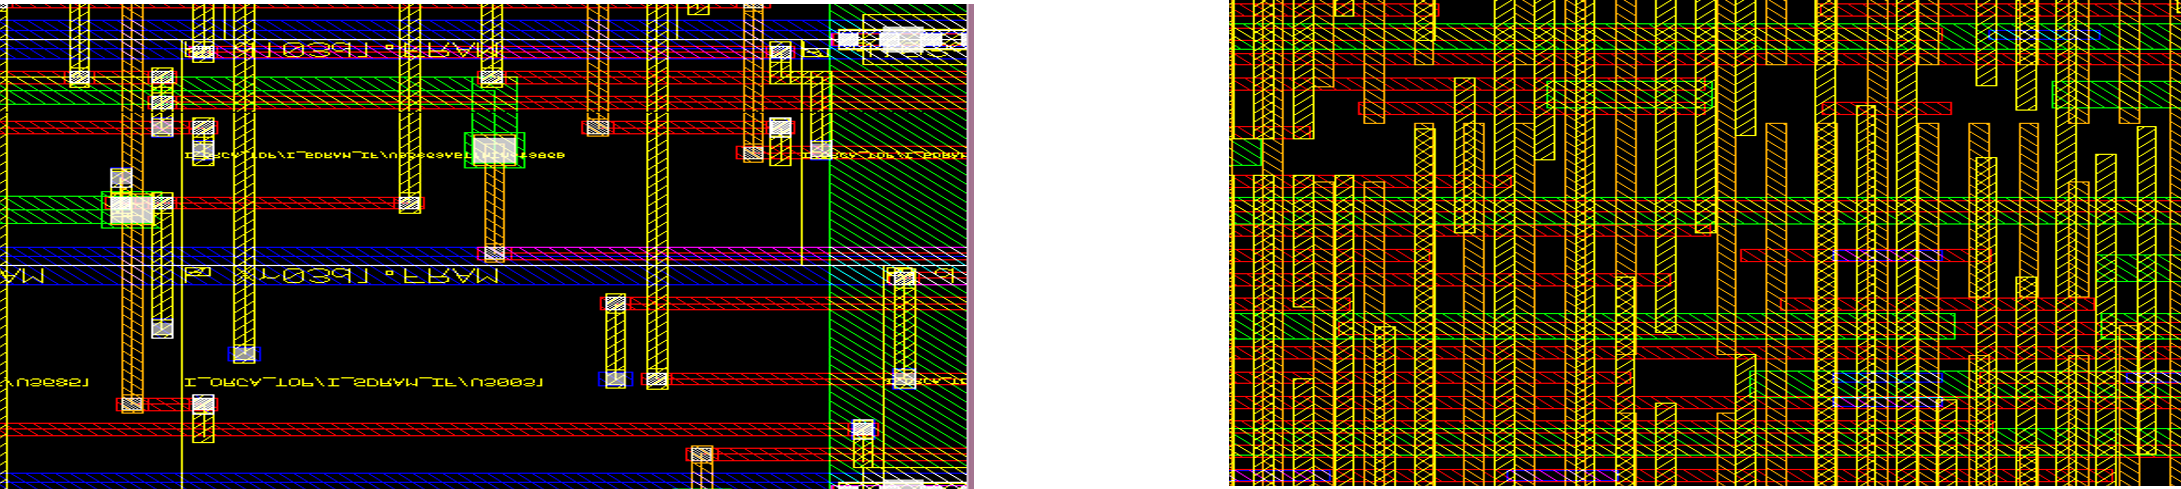
\includegraphics[width=0.8\textwidth]{Fill}
\end{center}
\begin{itemize}
	\item \textbf{Metal filling is done to improve process planarization, which is important for processes with a large number of metal layers.}
\end{itemize}
\end{frame}

\subsection[Slotting]{Metal Slotting}
\begin{frame}
	\frametitle{Problem: Metal Erosion}
	\begin{itemize}
		\item \textbf{The wafer is made flat (planarized) by a process
		called Chemical Mechanical Polishing (CMP)}
	\item \textbf{Metals are mechanically softer than dielectrics:}
	\begin{itemize}
		\item CMP leaves metal tops with a concave shape - \textbf{\underline{dishing}}
		\item The wider the metal the more pronounced the dishing
		\item Wide traces with little intervening dielectric and can
		become quite thin – dishing this severe is called \textbf{\underline{erosion}}
	\end{itemize}
	\item \textbf{Process rules specify \underline{maximum} metal density per
	layer to minimize erosion}
	\end{itemize}
\begin{center}
	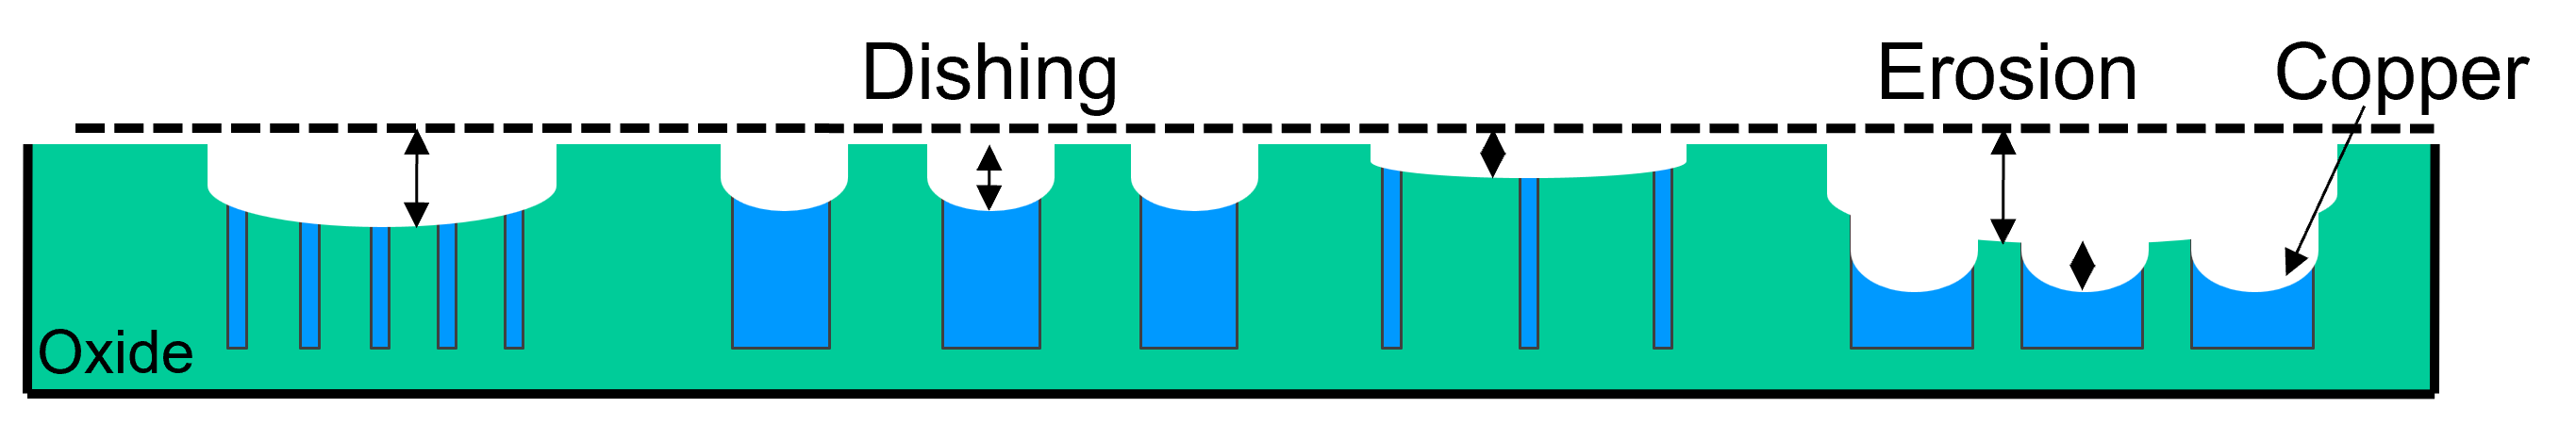
\includegraphics[width=\textwidth]{Erosion}
\end{center}
\end{frame}

\begin{frame}
	\frametitle{Problem: Metal Liftoff}
	\begin{itemize}
		\item \textbf{Conductors and Dielectrics have different coefficients
		of thermal expansion:}
	\begin{itemize}
		\item Stress builds up with temperature cycling
		\item Metals can delaminate (lift off) with time
		\item Wide metal traces are more vulnerable than narrow ones
	\end{itemize}
		\item \textbf{Maximum metal density rules also address this issue}
	\end{itemize}
\begin{center}
	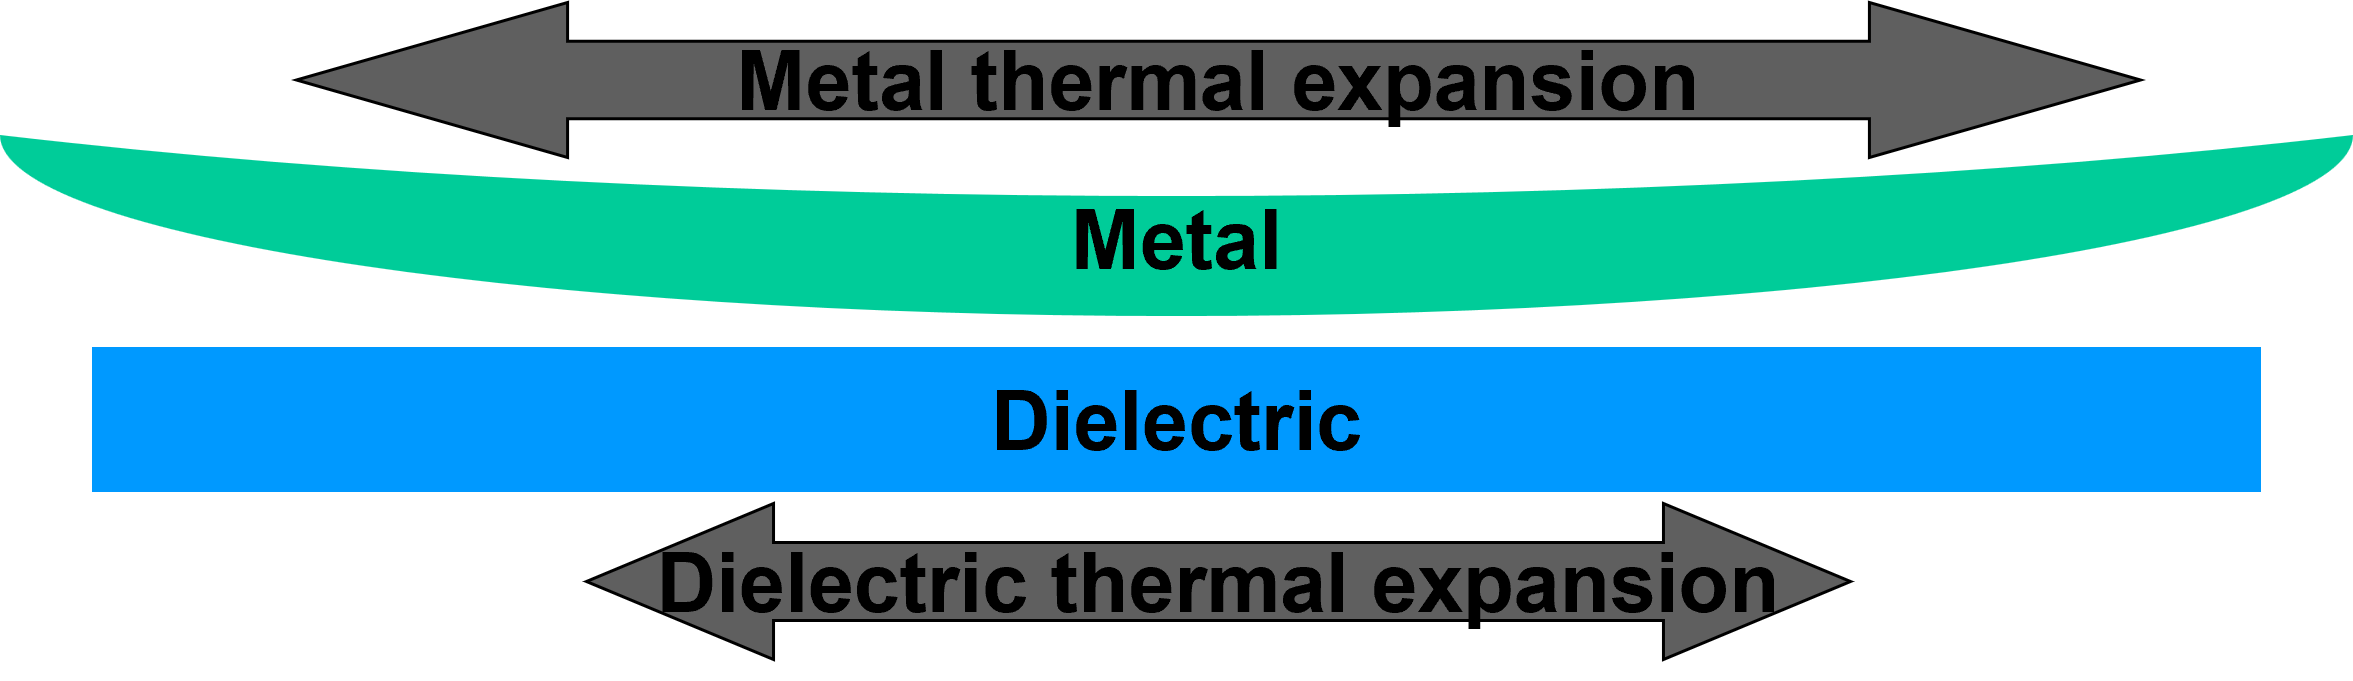
\includegraphics[width=\textwidth]{Liftoff}
\end{center}
\end{frame}

\begin{frame}
	\frametitle{Solution: Metal Slotting}
	\begin{itemize}
		\item Slotting wide wires reduces the metal density
		\item Slots minimize stress buildup, reducing liftoff
		tendency
		\item Primarily used on Power and Ground traces:
		\begin{itemize}
			\item Can apply to any other net if wide enough
		\end{itemize}
		
		\item Slotting parameters can be set layer by layer
	\end{itemize}
	\begin{center}
		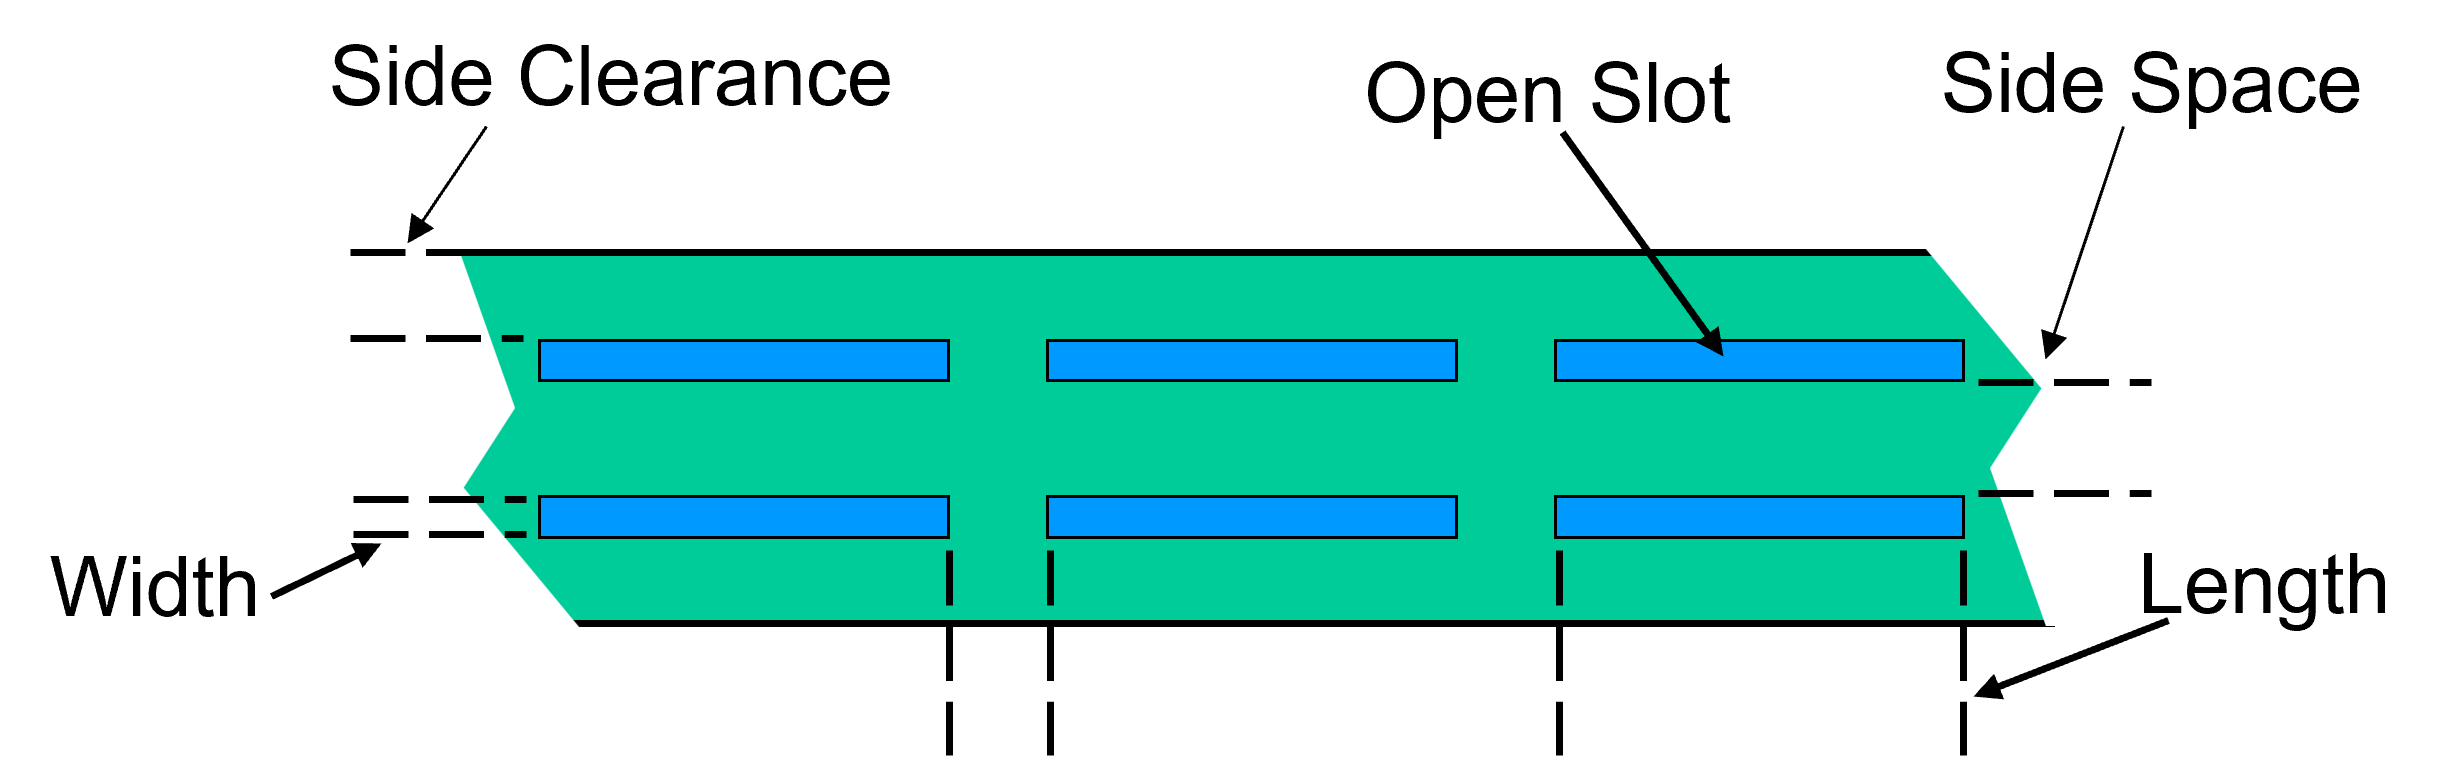
\includegraphics[width=\textwidth]{Slotting}
	\end{center}
\end{frame}

\subsection[Validation]{Final Validation}
\begin{frame}
	\frametitle{Final Validation}
	\begin{center}
		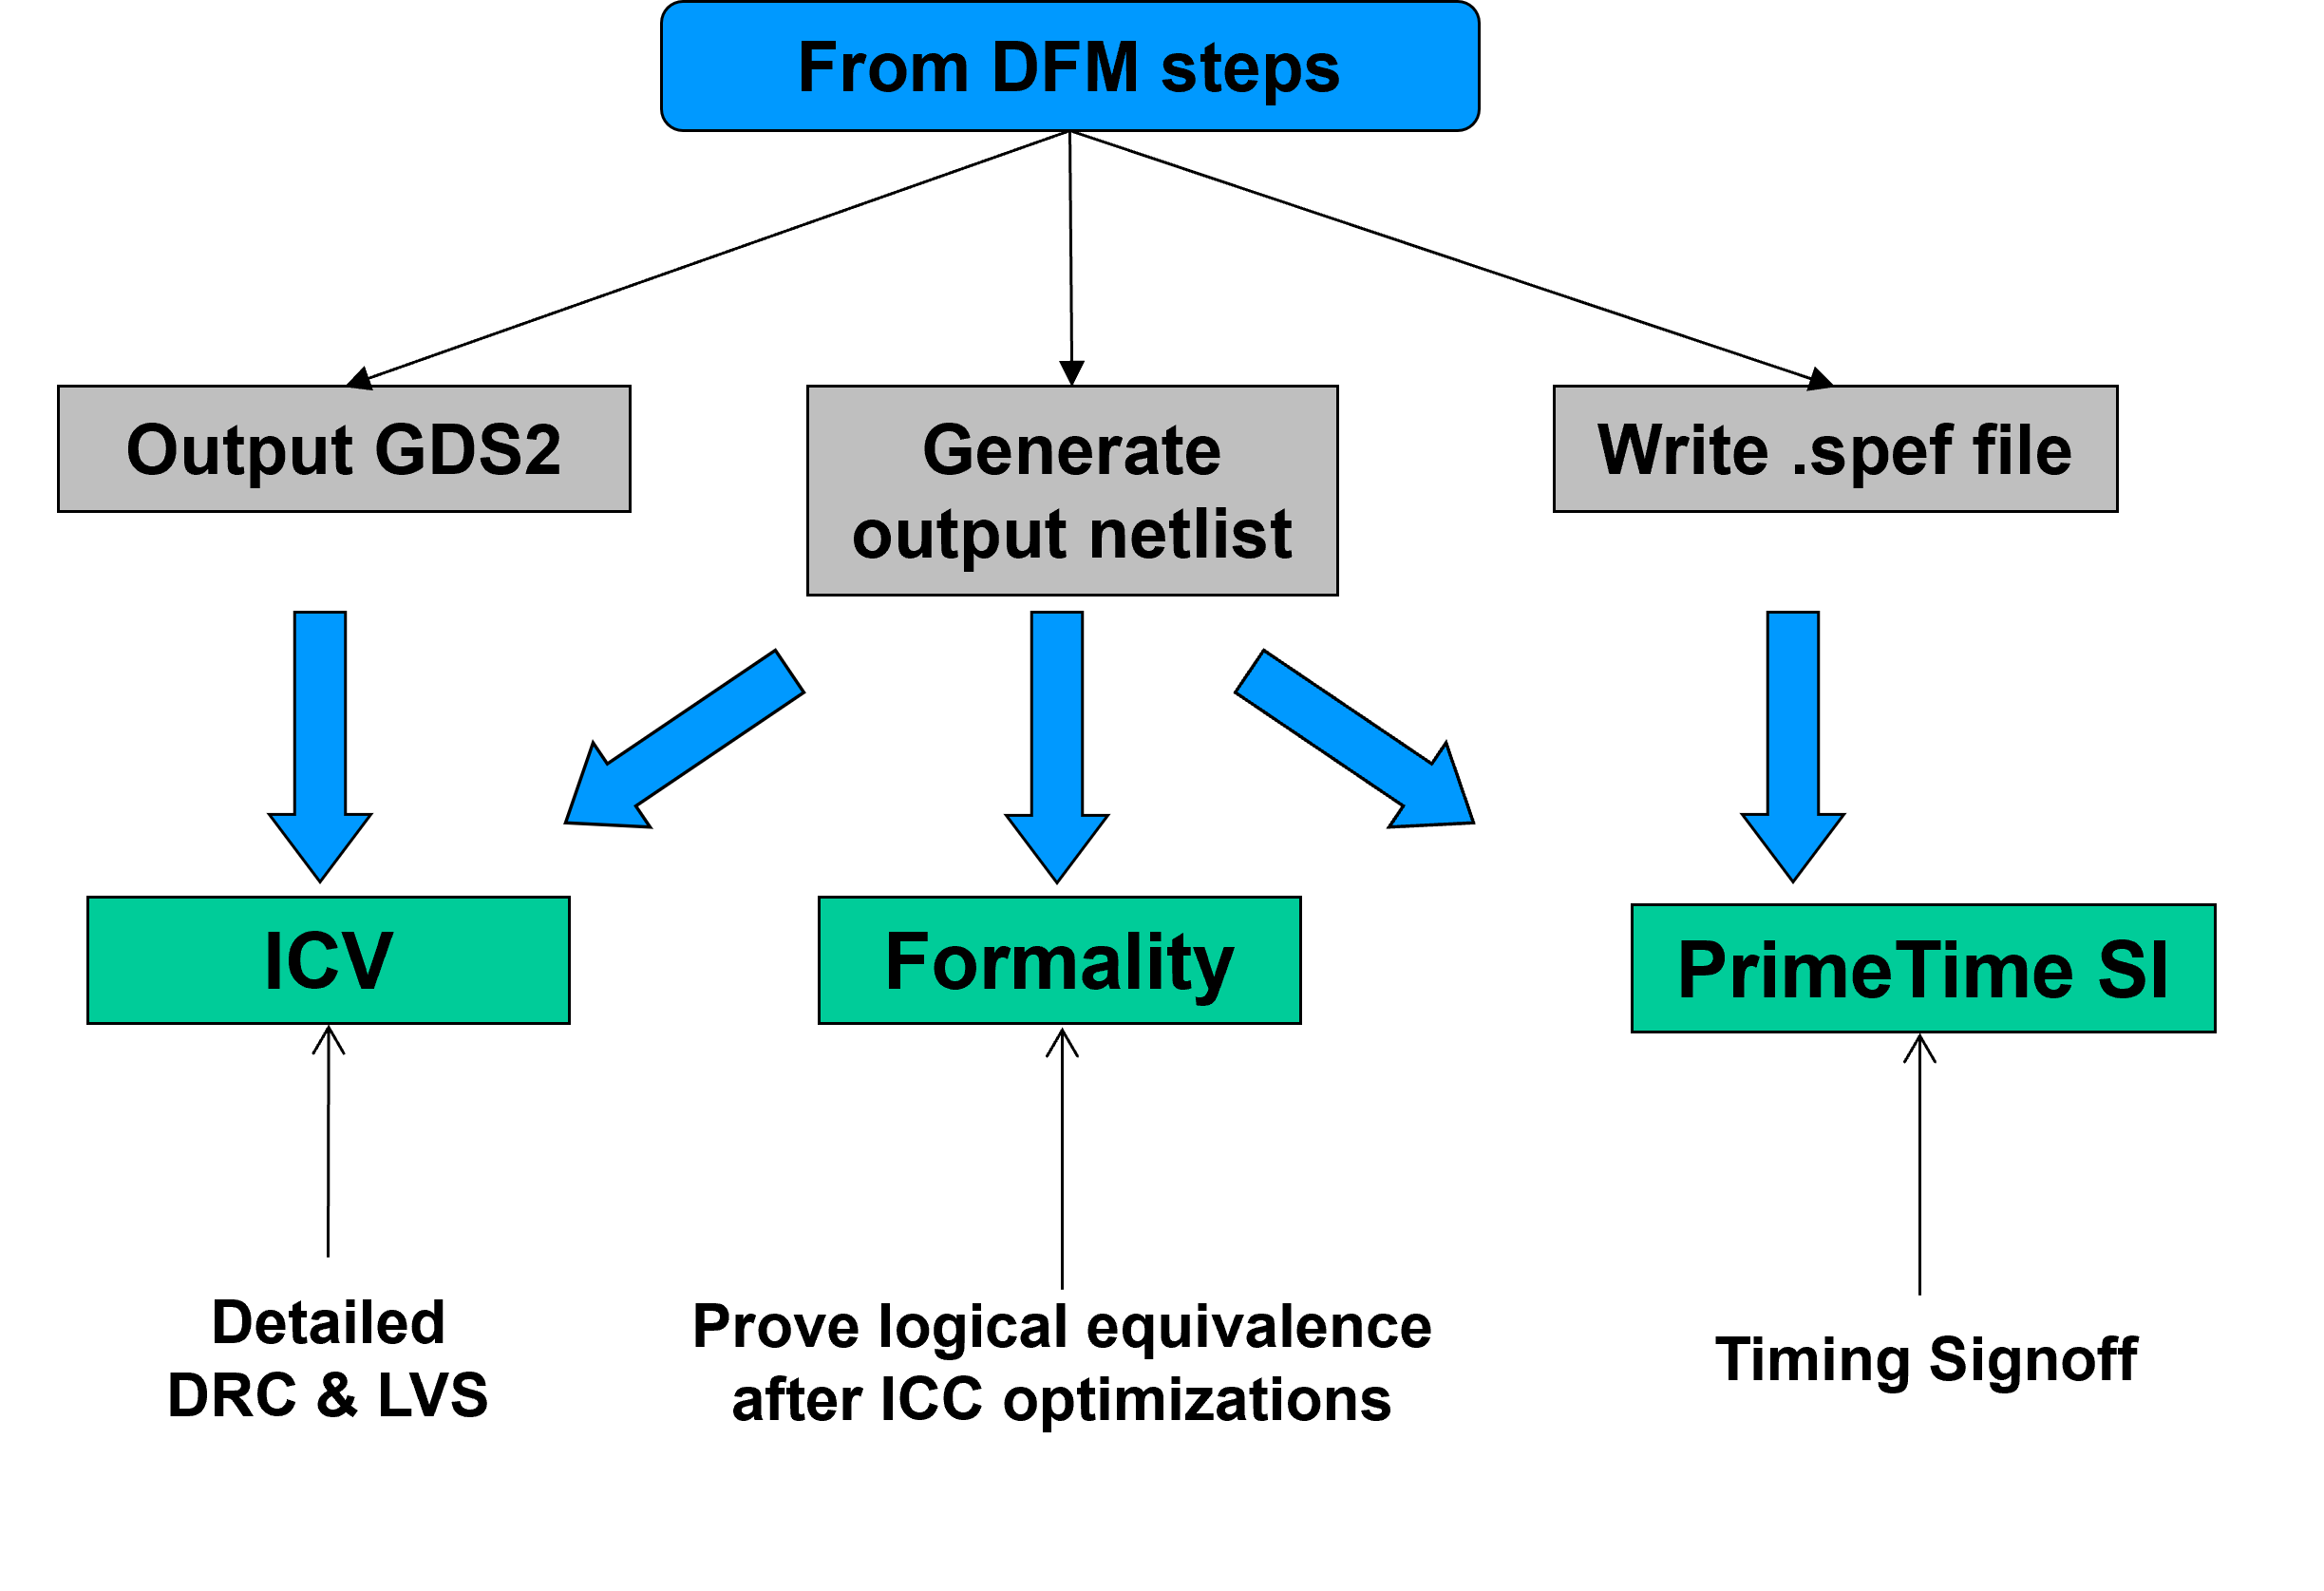
\includegraphics[width=\textwidth]{Validation}
	\end{center}
\end{frame}
%---------------------------------------------------	
	\begin{frame}
		\frametitle{....}
		\begin{center}
			\<بِسْمِ اللَّـهِ الرَّحْمَـٰنِ الرَّحِيمِ> \\
			\<وَمَا أُوتِيتُمْ مِنَ الْعِلْمِ إِلَّا قَلِيلًا>
			
		\end{center}
	\end{frame}
	%---------------------------------------------	
\end{document}	